%%%%% STYLES AND STUFF 
\documentclass[a4paper,oneside,onecolumn,openright,12pt]{book}


\makeatletter

%
\usepackage{caption}
\usepackage{subcaption}
\usepackage{footmisc}
\usepackage{paralist}
\usepackage{amsthm}
\usepackage{subfig}

% Fonts, encoding, etc.
\usepackage{type1cm}
\usepackage[latin1]{inputenc}
\usepackage[british]{babel}
\usepackage[T1]{fontenc}
\usepackage{times}
\usepackage{hyperref}
\usepackage[all]{hypcap}
\usepackage{longtable}
\usepackage{algorithm}
\usepackage{algpseudocode}
\usepackage{multirow}
\usepackage{float}


% Line spacing
\def\baselinestretch{1.5}
\parindent0cm
\parskip1.5ex\@plus.7ex\@minus.1ex\relax

%Acronyms
 \usepackage{acronym}
 %Inline lists
 \usepackage{paralist}

%Glossary
\usepackage[toc]{glossaries}

% Page dimensions
\usepackage{vmargin}
\setpapersize{A4}
\setmarginsrb{40mm}{20mm}{25mm}{30mm}{14.5pt}{8mm}{0pt}{11mm}

% Footer and header
\usepackage{afterpage}
\usepackage{fancyhdr}
\pagestyle{fancy}
\fancyhead{}
\fancyhead[LE,RO]{\thepage}
\fancyhead[LO,RE]{\slshape \leftmark}
\fancyfoot{}
\renewcommand{\chaptermark}[1]{}
\renewcommand{\sectionmark}[1]%
             {\markboth{\thesection\ #1}{\thesection\ #1}}
\renewcommand{\subsectionmark}[1]{}
\fancypagestyle{plain}{%
  \fancyhead{}
  \fancyhead[LE,RO]{\thepage}
  \fancyfoot{}
  \renewcommand{\headrulewidth}{.6pt}
}

% Chapter
\def\@makechapterhead#1{%
  \ \\[-35.5pt]\hbox to \textwidth {%
    \hfill {\vbox{\hbox{\rule[5pt]{140pt}{4pt}}%
        \hbox to 140pt {\hfill\huge\bfseries\slshape \@chapapp\space\thechapter\/}}}}%
  \vskip55\p@%
  {\parindent \z@ \raggedright \normalfont%
    \interlinepenalty\@M%
    \Huge \bfseries #1\par\nobreak%
    \vskip 45\p@%
  }}
\def\@chapter[#1]#2{\ifnum \c@secnumdepth >\m@ne
                       \if@mainmatter
                         \refstepcounter{chapter}%
                         \typeout{\@chapapp\space\thechapter.}%
                         \addcontentsline{toc}{chapter}%
                                   {\protect\numberline{\thechapter}#1}%
                       \else
                         \addcontentsline{toc}{chapter}{#1}%
                       \fi
                    \else
                      \addcontentsline{toc}{chapter}{#1}%
                    \fi
                    \chaptermark{#1}%
                    \addtocontents{lof}{\protect\addvspace{10\p@}}%
                    \addtocontents{lot}{\protect\addvspace{10\p@}}%
                    \addtocontents{loa}{\protect\addvspace{10\p@}}%
                    \if@twocolumn
                      \@topnewpage[\@makechapterhead{#2}]%
                    \else
                      \@makechapterhead{#2}%
                      \@afterheading
                    \fi}
\def\@schapter#1{\addcontentsline{toc}{chapter}{#1}%
                 \markboth{#1}{#1}%
                 \addtocontents{lof}{\protect\addvspace{10\p@}}%
                 \addtocontents{lot}{\protect\addvspace{10\p@}}%
                 \addtocontents{loa}{\protect\addvspace{10\p@}}%
                 \if@twocolumn%
                    \@topnewpage[\@makeschapterhead{#1}]%
                 \else%
                    \@makeschapterhead{#1}%
                    \@afterheading%
                 \fi}
\def\@makeschapterhead#1{%
  \ \\[-35.5pt]\hbox to \textwidth {%
    \hfill {\vbox{\hbox{\rule[5pt]{140pt}{0pt}\rule[5pt]{0pt}{4pt}}%
        \hbox to 140pt {\hfill\huge\bfseries\slshape \ \/}}}}%
  \vskip55\p@%
  {\parindent \z@ \raggedright \normalfont%
    \interlinepenalty\@M%
    \Huge \bfseries  #1\par\nobreak%
    \vskip 45\p@%
  }}

% Table of contents
\def\contentsname{Contents}
\renewcommand\tableofcontents{%
    \if@twocolumn%
      \@restonecoltrue\onecolumn%
    \else%
      \@restonecolfalse%
    \fi%
    \chapter*{\contentsname}%
    \@starttoc{toc}%
    \if@restonecol\twocolumn\fi%
    }

% Bibliography
\renewenvironment{thebibliography}[1]
     {\chapter*{\bibname}%
      \list{\@biblabel{\@arabic\c@enumiv}}%
           {\settowidth\labelwidth{\@biblabel{#1}}%
            \leftmargin\labelwidth
            \advance\leftmargin\labelsep
            \@openbib@code
            \usecounter{enumiv}%
            \let\p@enumiv\@empty
            \renewcommand\theenumiv{\@arabic\c@enumiv}}%
      \sloppy
      \clubpenalty4000
      \@clubpenalty \clubpenalty
      \widowpenalty4000%
      \sfcode`\.\@m}
     {\def\@noitemerr
       {\@latex@warning{Empty `thebibliography' environment}}%
      \endlist}

% Floats
\long\def\@makecaption#1#2{%
  \vskip\abovecaptionskip
  \sbox\@tempboxa{\textbf{#1: #2}}%
  \ifdim \wd\@tempboxa >\hsize
    \textbf{#1: #2.}\par
  \else
    \global \@minipagefalse
    \hb@xt@\hsize{\hfil\box\@tempboxa\hfil}%
  \fi
  \vskip\belowcaptionskip}
\renewcommand{\topfraction}{0.9}
\renewcommand{\textfraction}{0.1}
\renewcommand{\floatpagefraction}{0.9}

% Tables
\usepackage{dcolumn}
\usepackage{hhline}

% Graphics
\usepackage[dvips]{graphicx}
\usepackage[usenames,dvipsnames]{color}
\usepackage{rotating}
\usepackage{psfrag}
\usepackage{epic}
\usepackage{eepic}


% List of figures and tables
\renewcommand\listoffigures{%
    \if@twocolumn
      \@restonecoltrue\onecolumn
    \else
      \@restonecolfalse
    \fi
    \chapter*{\listfigurename}%
      \@mkboth{\listfigurename}{\listfigurename}%
    \@starttoc{lof}%
    \if@restonecol\twocolumn\fi
    }
\renewcommand\listoftables{%
    \if@twocolumn
      \@restonecoltrue\onecolumn
    \else
      \@restonecolfalse
    \fi
    \chapter*{\listtablename}%
      \@mkboth{\listtablename}{\listtablename}%
    \@starttoc{lot}%
    \if@restonecol\twocolumn\fi
    }

% Math symbols, fonts, etc.
\usepackage{amsmath}
\usepackage{amsfonts}
\usepackage{amssymb}

\newcommand{\N}{\mathbb{N}}
\newcommand{\Z}{\mathbb{Z}}
\newcommand{\Q}{\mathbb{Q}}
\newcommand{\R}{\mathbb{R}}
\newcommand{\C}{\mathbb{C}}
\renewcommand{\S}{\mathbb{S}}
\renewcommand{\P}{\mathbb{P}}
\newcommand{\E}{\mathbb{E}}

\newcommand{\Cf}{\mathfrak{C}}
\newcommand{\Pf}{\mathfrak{P}}

\DeclareMathOperator{\sign}{sign}
\DeclareMathOperator{\avg}{avg}
\DeclareMathOperator{\floor}{floor}
\DeclareMathOperator{\ceil}{ceil}
\DeclareMathOperator{\round}{round}

\providecommand{\abs}[1]{\lvert#1\rvert}
\providecommand{\absd}[1]{\left\lvert#1\right\rvert}
\providecommand{\card}[1]{\lvert#1\rvert}
\providecommand{\norm}[1]{\lVert#1\rVert}

% URLs
\usepackage{url}
%% Define a new 'leo' style for the package that will use a smaller font.
\makeatletter
\def\url@leostyle{%
  \@ifundefined{selectfont}{\def\UrlFont{\sf}}{\def\UrlFont{\footnotesize\ttfamily}}}
\makeatother
%% Now actually use the newly defined style.
\urlstyle{leo}




% STUFF I ADDED:

\usepackage{thmbox}
\newtheorem[S,leftmargin=18pt,thickness=0.9pt,bodystyle=\noindent]{mydefinition}{Definition}[chapter]
\newtheorem[S,leftmargin=18pt,thickness=0.9pt,bodystyle=\noindent]{myproposition}{Proposition}[chapter]
\newtheorem[S,leftmargin=18pt,thickness=0.9pt,bodystyle=\noindent]{myobservation}{Observation}[chapter]

\usepackage{amssymb}
\usepackage{graphicx}
\usepackage{float}
\usepackage{pgfplots}
\usepackage{pgfplotstable}
\pgfplotsset{
    % #1: index in the group(0,1,2,...)
    % #2: number of plots of that group
    bar group size/.style 2 args={
        /pgf/bar shift={%
                % total width = n*w + (n-1)*skip
                % -> subtract half for centering
                -0.5*(#2*\pgfplotbarwidth + (#2-1)*\pgfkeysvalueof{/pgfplots/bar group skip})  + 
                % the '0.5*w' is for centering
                (.5+#1)*\pgfplotbarwidth + #1*\pgfkeysvalueof{/pgfplots/bar group skip}},%
    },
    bar group skip/.initial=2pt,
    plot 0/.style={blue,fill=blue!30!white,mark=none},%
    plot 1/.style={red,fill=red!30!white,mark=none},%
    plot 2/.style={brown!60!black,fill=brown!30!white,mark=none},%
}

\usepackage{listings}
\usepackage{color}
\lstset{ %
  language=Octave,                % the language of the code
  basicstyle=\footnotesize\ttfamily,           % the size of the fonts that are used for the code
  numbers=left,                   % where to put the line-numbers
  numberstyle=\tiny\color{black},  % the style that is used for the line-numbers
  stepnumber=2,                   % the step between two line-numbers. If it's 1, each line 
                                  % will be numbered
  numbersep=5pt,                  % how far the line-numbers are from the code
  backgroundcolor=\color{white},      % choose the background color. You must add \usepackage{color}
  showspaces=false,               % show spaces adding particular underscores
  showstringspaces=false,         % underline spaces within strings
  showtabs=false,                 % show tabs within strings adding particular underscores
  rulecolor=\color{black},        % if not set, the frame-color may be changed on line-breaks within not-black text (e.g. commens (green here))
  tabsize=3,                      % sets default tabsize to 3 spaces
  captionpos=b,                   % sets the caption-position to bottom
  breaklines=true,                % sets automatic line breaking
  breakatwhitespace=false,        % sets if automatic breaks should only happen at whitespace
                                  % also try caption instead of title
  keywordstyle=\color{blue},          % keyword style
  commentstyle=\color{dkgreen},       % comment style
  stringstyle=\color{mauve}      % string literal style
}


% FUNCTIONS:

% retweet group
\newcommand{\rg}[1]{RG(#1)}

% retweets 
\newcommand{\rt}[1]{RT(#1)}

% retweet count
\newcommand{\rc}[1]{#1.\textrm{count}_R}

% expected retweet count
\newcommand{\ec}[1]{e(#1)}
\newcommand{\ecg}[1]{e_G(#1)}
\newcommand{\ecu}[1]{e_U(#1)}

% follower count
\newcommand{\foc}[1]{\textrm{deg}^+(#1)}

% friend count
\newcommand{\frc}[1]{\textrm{deg}^-(#1)}

% author
\newcommand{\aut}[2]{#1.\textrm{author}_#2}

% set of followers
\newcommand{\fos}[1]{N^+(#1)}

% set of friends
\newcommand{\frs}[1]{N^-(#1)}

% raw audience
\newcommand{\raa}[1]{\textrm{audience}(#1)}

% distinct audience
\newcommand{\dia}[1]{\textrm{audience}(#1)}

% interestingness score
\newcommand{\score}[1]{s(#1)}
\newcommand{\gscore}[1]{s_G(#1)}
\newcommand{\uscore}[1]{s_U(#1)}
\newcommand{\ascore}[1]{s_{\textrm{avg}}(#1)}

% score disparity
\newcommand{\disparity}[1]{d(#1)}
\newcommand{\gdisparity}[1]{d_G(#1)}
\newcommand{\udisparity}[1]{d_U(#1)}
\newcommand{\sdisparity}[1]{d_{\textrm{sel}}(#1)} % disparity between SELECTED tweets in question #1

% END OF STUFF I ADDED

\makeatother


\begin{document}


%%%%% FRONT STUFF	
\frontmatter

\begin{titlepage}

\begin{center}
\vspace*{3ex}
\textbf{\Huge Inferring Interestingness in Online Social Networks}\\[2ex]

\textbf{\LARGE William M. Webberley}\\
\vfill
\textbf{\LARGE 2014}\\
\vfill
\textbf{\LARGE Cardiff University}\\[1ex]
\textbf{\LARGE School of Computer Science \& Informatics}\\[4ex]
\end{center}

\end{titlepage}

\newpage\thispagestyle{empty}\cleardoublepage


\thispagestyle{plain}

\vspace*{6ex}

\textbf{\large Declaration}

This work has not previously been accepted in substance for any degree and is not concurrently submitted in candidature for any degree.\\[2ex]
Signed \dotfill \ (candidate) \hspace*{10em}\\[1ex]
Date\ \ \ \ \ \dotfill \hspace*{18em}

\vfill

\textbf{\large Statement 1}

This thesis is being submitted in partial fulfillment of the requirements for the degree of PhD.\\[2ex]
Signed \dotfill \ (candidate) \hspace*{10em}\\[1ex]
Date\ \ \ \ \ \dotfill \hspace*{18em}

\textbf{\large Statement 2}

This thesis is the result of my own independent work/investigation,
except where otherwise stated. Other sources are acknowledged by
explicit references.\\[2ex]
Signed \dotfill \ (candidate) \hspace*{10em}\\[1ex]
Date\ \ \ \ \ \dotfill \hspace*{18em}

\vfill

\textbf{\large Statement 3}

I hereby give consent for my thesis, if accepted, to be available for photocopying and for inter-library loan,
 and for the title and summary to be made available to outside organisations.\\[2ex]
Signed \dotfill \ (candidate) \hspace*{10em}\\[1ex]
Date\ \ \ \ \ \dotfill \hspace*{18em}

\vfill

\cleardoublepage


\thispagestyle{plain}
\ \vfill{\small
Copyright \copyright\ 2014 Will Webberley.\\
Permission is granted to copy, distribute and/or modify this document
under the terms of the GNU Free Documentation License, Version 1.3\footnote{http://www.gnu.org/copyleft/fdl.html} or
any later version published by the Free Software Foundation; with no
Invariant Sections, no Front-Cover Texts, and no Back-Cover Texts}\\[3.5ex]
\cleardoublepage


\ \vspace*{1.11cm}
\markboth{Dedication}{}
\begin{flushright}
%\textbf{\large To my parents, family and friends;}\\
%\textbf{\large To George, Pete,}\\
%\textbf{\large Jack, Max, Ella,}\\
%\textbf{\large Tom, and Charlie.}\\
%\large This is for their patience and support.
\end{flushright}
\newpage
\markboth{}{}
\cleardoublepage

\chapter*{Acknowledgements}
% Finish this section and tidy up, etc.

%This thesis and the research it contains would not exist if it weren't for the unfailing support of my supervisors, Roger Whitaker and, particularly, Stuart Allen. Their guidance and input have provided drive and shaped my research and have given me the confidence required in producing and defending ideas both within and outside of research. My utmost gratitude is extended to them for this and for their continuing encouragement at all stages of the PhD, always with fresh ideas and clarification for research pathways and for keeping me on track. I feel confident in saying that I was very lucky in being in their supervision and I would not be the same person, professionally and otherwise, today if it wasn't for their combined inputs over the past few years.

%I'd also like to lend my thanks to Martin Chorley for his continuously helpful and enthusiastic crowdsourcing expertise, without which the research in this thesis could not have been validated in the way it has. Matt Williams has provided insight throughout my time as a PhD student, from long sessions discussing the tiniest details to recommendations on research direction and scope. His ideas have helped shape many of the notions in this thesis. I am also deeply grateful to Chris Gwilliams for his inputs and support for everything; from where one might find the most effective M.O.T. deals through to how best to structure complex and fiddly data queries. He deserves far more than a simple acknowledgdment.

%Finally, my time as a research student would not have been the same without the constant presence and support from the other members of the MobiSoc group, the `superteam' and my non-academic friends. Gualtiero Colombo, Ian Cooper, Matt John, Liam Turner, Nick Sharp, and Ross Taylor have all provided assistance and I am very theankful to them for putting up with my worries and fusses without complaint.

%Thanks, all.



\chapter*{Abstract}
Information sharing on the Internet has given rise to the increased presence of non-interesting and `noisy' information in media streams on many online social networks. Although there is, however, a lot of `interesting' information also shared amongst users, the noise increases the cognitive burden in terms of the users' abilities to identify the interesting information and may affect the chance of the user missing important or interesting information. 
Additionally, users on such platforms are generally limited to receiving information only from those that they are directly linked to on the social graph, meaning that users exist within distinct information `bubbles', further limiting the chance of receiving interesting and relevant information from outside of the immediate social circle. 
In this thesis, Twitter is used as a platform for researching methods for deriving information ``interestingness'' through information popularity as given by the mechanism of \textit{retweeting}, which allows information to be propagated further between users on Twitter's social graph. Retweet behaviours are studied, and various properties are uncovered which relate retweet action to the social graph. This culminates in research into a methodology for assigning scores to Tweets based on their `quality', which is validated to perform well in various situations, and is analysed to demonstrate its potential in highlighting interesting information in mixed information streams.


\tableofcontents
\newpage
\chapter*{List of Publications}

Some of the work produced towards this thesis has also been published separately as follows.

\begin{itemize} 

\item \cite{webberley13} - W. Webberley, S. M. Allen, R. M. Whitaker. \textit{Inferring the Interesting Tweets in Your Network}, 
			in \textit{Workshop on Analyzing Social Media for the Benefit of Society (SOCIETY 2.0), 3\textsuperscript{rd} International Conference on Social Computing and its Applications (SCA)},
			Karlsruhe, Germany. \textit{IEEE 2013} 

\item \cite{webberley11} - W. Webberley, S. Allen, R. Whitaker. \textit{Retweeting: A Study of Message-Forwarding in Twitter}, 
			in \textit{Workshop on Mobile and Online Social Networks (MOSN'11), 5\textsuperscript{th} International Conference on Network and System Security (NSS)},
			Milan, Italy. \textit{IEEE 2011}

\end{itemize}

\listoffigures
\listoftables
\chapter*{List of Acronyms} 
\begin{acronym}
% to use in the thesis, use: \ac{OSN}
\acro{OSN}{Online Social Network}
\acro{MTW}{Mechanical Turk Worker}
\acro{URL}{Uniform Resource Locator}

\end{acronym}

\chapter*{Glossary} 

{\bf Follower}
A type of user. A user, \textit{x}, is a follower of user \textit{y} if user \textit{x} follows user \textit{y}. Other users who follow a particular user will receive all of the user's Tweets and retweets to their home timeline. A user can elect to follow another user.

{\bf Friend}
The inverse of follower. User \textit{x} is a friend to user \textit{y} if \textit{y} follows \textit{x}.

{\bf Path-length}
The penetration of a Tweet - i.e. the number of times a Tweet is retweeted down one chain. The final retweeter in the chain indicates the number of hops the Tweet has taken from its author.
			
{\bf Retweet}
\textit{n.} - A replica of a Tweet, which has been forwarded on by a user (who is not the Tweet's original author) to their own followers. \\
\textit{v.} - The act of replicating a Tweet. A user who finds a Tweet interesting may retweet it so that it gets more exposure.
									
{\bf Retweet Group}
Set of Twitter users responsible for the propagation of a Tweet. Comprises the original author of the Tweet and the users which have since retweeted it.

{\bf Retweet Count}
The number of times a particular Tweet has been retweeted.

{\bf Timeline}
A collection of Tweets in Twitter in reverse-chronological order. A user timeline consists of that user's Tweets. A user's home timeline consists of the Tweets of each friend of the user.

{\bf Tweet}
\textit{n.} - A piece of information in Twitter; a piece of text, less than 240 characters long, which is written by a user. When sent, the Tweet is sent to the home timelines of each of the followers of the Tweet's author.\\
\textit{v.} - The act of writing and sending a Tweet.

{\bf User}
An account on Twitter. Each user (usually representing a real-life person or organisation) can Tweet, retweet, follow other users and be followed by other users. In this thesis, sometimes the terms \textit{user} and \textit{person} are used interchangeably.

%%%%% MAIN STUFF 
\mainmatter 

\chapter{Introduction}

Online social networks have exploded into the lives of millions of people worldwide over the last decade, and their use has dominated the communication highways and facilitated the interconnection of the world in ways never before perceived possible.

These social networks imitate real-world social networks. Although most such platforms each provide a different service to collaboratively satisfy an array of different use-cases, they tend to all be based around the idea of `friendships' (i.e. links between the user nodes in the social graph) and the sharing of information amongst friends.

Social networks like these have been available for around ten years now (with MySpace\footnote{http://myspace.com} launching in 2003 and Bebo\footnote{http://bebo.com} in 2005), but it wasn't really until Facebook's\footnote{http://facebook.com} worldwide launch in 2006 that social networks became the staple, ubiquitous norm that they are today. More recently, we have seen the introductions of Google's social network grown from its Buzz service, Google Plus\footnote{http://plus.google.com}, Pinterest\footnote{http://pinterest.com}, App.net\footnote{http://app.net}, and many more. They make up a large part of the basis and meaning behind the ideas of Web 2.0, which describes the web as being primarily formed from user-generated content and encourages the sharing of such content.

Another component that helped in the dawn of Web 2.0 was the rise of \textit{blogging}. A blog (`web-log') is a time-based series of posts consisting of continuous pieces of text, photos, or other media, and is generally contributed to by a single author. Blogs are often based around one or a set of topics and are usually public - meaning that they are written with the intention of being read by others. Despite this, they are often a way in which the author can look back at their history of posts, acting more as a diary recording snapshots of the author's life.\\
Various blogging services exist on the web today, such as Medium\footnote{http://medium.com}, Wordpress\footnote{http://wordpress.com}, and Tumblr\footnote{http://tumblr.com}.


\section{Twitter as a Social Network}
Twitter\footnote{http://twitter.com} is an online social network, which launched in the summer of 2006 \cite{krishnamurthy08}. Since then, it has rapidly gained in popularity amongst several different user groups - teens and young people, casual users, celebrities, reporters, and so on - and within eight months had around 94,000 registered users \cite{java07}. Although Twitter has never been a direct competitor with Facebook, users tend to use the two sites concurrently for different purposes: whilst Facebook's focus is on providing many services at once (such as photo-sharing, commenting/endorsing of information, messaging, pages for businesses, groups, events, etc.), Twitter's is more on simplicity.

More specifically than just being an online social network, Twitter is a microblogging website. Whilst a blog, as mentioned, typically contains long posts, Twitter only allows its users to post short pieces of text, up to 140 characters in length \cite{krishnamurthy08} \cite{huberman08}, called `Tweets'. Thus, Twitter is a hybrid social network and blogging service and whilst each Tweet may only realistically be able to hold a couple of sentences, this system facilitates quick, timely, and `real-time' \textit{live} information-sharing amongst its millions of users \cite{zhao09}. Its idea is that short pieces of news will `travel' faster and will be seen by more people more quickly than traditional news stories.

Although Tweets are limited to 140 characters in length, the inclusion of URLs is allowed. This enables further extension of Tweets through external websites, and supports the inclusion of links to images and videos. Twitter has encouraged this use-case by providing `share' buttons for developers to embed in websites, and direct support for photo and video applications, such as TwitPic\footnote{http://twitpic.com} and Vine\footnote{http://vine.com}.

Its simplicity has also helped its growth into the mobile domain, in which smartphone users are able to very quickly post updates about their lives, a piece of information they want to share, or a photo or video, and be able to post it \textit{as it happens} directly from the news source or geographical location \cite{castillo11}. This has been especially useful in emergency situations worldwide, including the Haiti earthquake in 2010 \cite{muralidharan11}, and 2011's Egyptian protests \cite{wilson11} and Thai flood \cite{kongthon12}.\\
Indeed, \cite{sakaki10} used Twitter to build an earthquake-reporting system for Japan that outperforms the Japan Meteorological Agency in terms of its promptness of notification.

Use of Twitter is based around `timelines' of Tweets, to which new Tweets are pre-pended as they are posted by users. The \textit{home} timeline is the default view, in which Tweets from all of a person's subscribed-to users are placed. Timelines of an individual user contain only Tweets from that user, and are known as a `user' timeline. Customisation of timelines is also possible through the use of Twitter lists, in which different users can be placed to categorise streams of Tweets from different sets of users.


\section{Twitter's Social Graph and Information Subscription}
As with many social networks, the structure of Twitter lies within the users and their connectivity within its social graph. However, unlike Facebook, whose social structure is made up of bi-directional `friendships' between users, Twitter's primary social graph is made up more of mono-directional links between its users \cite{edwards13}. A person using Twitter can elect to \textit{follow} another user, which subscribes the person to receive all of that user's Tweets to their home timeline. The set of users that follow a person are known as that person's \textit{followers}, and the set of users that the person follows are the person's \textit{friends}.\\
Therefore, if two users both mutually follow each other, then the link between them is bi-directional.

Whilst bi-directional links are common amongst communities of similar interests, friends, colleagues, and so on, mono-directional links are found more in situations in which less-influential users follow more-influential users, such as celebrities.


\section{The Problem}
A user who follows a set of other users can \textit{generally} be said to find that set of users to produce more interesting information than those users that the user does not follow. However, despite that, not \textit{all} information produced by an `interesting' user is likely to be interesting, and yet \textit{all} information produced by a Twitter friend will be received onto the home timeline.\\
Noise is a common problem in Twitter, and is the uninteresting information one might receive that conveys little interest. It is likely that most of the information received on Twitter \textit{is} uninteresting \cite{alonso10}, and this makes it very hard to distinguish the interesting information from the uninteresting.

Since people tend to use Twitter most in short sporadic moments, looking for a quick news fix, they do not have time to filter out noisy information. Thus, the presence of noise can dampen the experience of the user, making it much more difficult to find interesting information.

In addition, Twitter users typically exist within an information `bubble'. This is similar to the notion of the Google search bubble, in which the search engine uses previous results and search terms to only return information to a user based on what \textit{it thinks} the user would find the most interesting and useful.\\
This results in the users not knowing which information exists beyond the confines of their bubble, and if they do not know it exists, they cannot know if it is of interest to them. Similarly, a Twitter user cannot follow all of the users he/she may find interesting, since he/she will not \textit{know} of all the interesting users existing on the social graph.

How can users be exposed to \textit{interesting} and \textit{relevant} information, but without them having to know about it or look for it first?


\section{Contributions}
This thesis focuses on understanding information propagation, and how this combined with knowledge of the social structure of Twitter can assist towards solving the problem of identifying interesting and relevant information and determining it from the noise on Twitter. 
Whilst other work in the area has also looked into the notions of relevance and interest in online social networks, and Twitter in particular, none has addressed the problem in such a way as this.

Part of the outcome of this research are methods for effectively inferring interesting information and, indeed, ranking information by interestingness. The methods are validated in various ways to help highlight their strengths and weaknesses in performing inferences and appropriate use-cases.

The work addresses the problem area in that it helps towards solving the goal of identifying \textit{globally} interesting information in Twitter. In addition, certain measures are taken in an attempt to address the idea of information relevance, which denotes how information interestingness is subjective, and thus different from user to user.


\section{Thesis Structure}
The rest of this thesis is structured as follows.

A background is provided as an introduction to some of the ideas behind the main research, which immediately follows this chapter, and includes a review of relevant literature across the range of topics addressed in the thesis.\\
Following this are chapters that contain research on Twitter's information propagation characteristics and its interesting and useful behaviours, the social structure of Twitter and the ways in which this is important for understanding the spread of information, and then on the research of the methodologies themselves, including validation and analysis of the results of this work.

The thesis ends with a general analysis and conclusion, and a discussion of potential future work in this area and leading on from this research.
\chapter{Background}


One of the most widely-used features of Twitter is its inbuilt function for facilitating the spread of information within its social structure. This phenomenon is the basis for much of the research in this thesis and, when combined with the characteristics of Twitter's user graph, has many interesting attributes and behaviours associated with it.


\section{Domain Context}

\subsection{Information Propagation through Retweeting}
The function of propagation in Twitter is known as \textit{retweeting}, and is carried out by the Twitter users themselves. When a user views a Tweet that they believe to be particularly interesting, and believe it to also be interesting to his/her followers, then he/she can elect to retweet it, and thus pass it further through the social graph to that user's followers also. A Tweet that has been retweeted is known as a \textit{retweet}, and it is clear that a Tweet which is retweeted will be made available to significantly more users than a Tweet that isn't retweeted \cite{webberley11} \cite{kwak10}.

Since Twitter's social graph is decentralised and retweeting occurs between individual groups of users, its properties are similar to information dissemination in other types of decentralised graphs, such as content-forwarding in opportunistic networking \cite{allen10}.

A retweet can be carried out in one of two ways: either through the use of Twitter's native retweet button, or manually. \\
The retweet button is displayed along with each Tweet in a Tweet timeline which, when clicked, immediately creates a new retweet containing the verbatim content of the original Tweet and automatically sends it on to the retweeter's followers.\\ The user who created the original Tweet is credited as the author on the recipients' timelines, with an indication of who carried out the retweet itself. Thus, users who follow the retweeter will see a Tweet appear in their home timeline from someone that they may not directly follow.\\

\begin{figure}[h]
\centering

\includegraphics[scale=0.3]{2.Background/Media/northern_lights_tweet.png} 
\caption{A retweeted Tweet}
\label{fig:northern_lights_tweet}
\end{figure}

The manual approach involves physically copying the content of the Tweet to be retweeted and pasting it into a new Tweet, usually with the text `\texttt{RT @<username>:}' pre-pended, where \texttt{RT} stands for \textbf{r}e\textbf{t}weet and \texttt{<username>} is the username of the author of the original Tweet. This method allows for annotating the original content of the Tweet (for example, to provide an opinion on the Tweet contents), producing a \textit{modified} Tweet, which can sometimes be pre-pended with \texttt{MT} rather than \texttt{RT}.

\begin{figure}[h]
\centering

\includegraphics[scale=0.3]{2.Background/Media/retweet_button.png} 
\caption{The retweet `button' in context}
\label{fig:retweet_button}
\end{figure}

Each Tweet has a retweet count associated with it, which is the raw representation of the number of times that the Tweet has been retweeted using the retweet button method.\\
Since the manual retweet technique is more community-driven, there is no official way to include these as part of the retweet count of the original Tweet. However, since the manual method is typically only really used with the aim to annotate or modify the Tweet in some way, the resultant `retweet'  is no longer a real representation of the content of the original Tweet anyway, and so should not be counted as such.

It should be noted that Twitter users may choose to make their account `protected'. A person who has a protected account will still have a publicly-visible profile (displaying a name, username, bio, and so on), but their Tweets and other information (such as the followers and friends lists) are hidden from users that aren't followers of the person. Potential followers of a protected account must \textit{request} a followship, which can then be accepted or rejected by the protected account holder. \\
Since Tweets from a protected account are only visible to approved followers, the retweet button is unavailable for them to disseminate the Tweet any further than the author's immediate local follower network. However, since the manual retweet method does not rely on the button and isn't governed by Twitter, a protected account's Tweets can still be retweeted in this way.

In a similar way to Facebook supporting the endorsement of information found on its site by inviting users to `like' a piece of content, retweeting is effectively a \textit{vote} or endorsement for a Tweet on Twitter. In both cases, the number of likes and number of retweets is visible to the platforms' respective users, and so this provides some insight into the \textit{popularity} of the information.\\


\subsection{Retweets and the Social Graph}
The social graph of Twitter is constructed, like in other online social networks, by edges between users, partially emulating real-life social interactions between humans. The growth of social media has encouraged more dense communication between users all over the world, who would not previously be able to be in direct contact with one another in this way.

Derived from this, Stanley Milgram's finding of ``six degrees of separation'' \cite{milgram67}, which defines that people are usually no more than six hops away from each other on the `real-life' social graph, was found to be an overestimate when it comes to the analysis of the structure of OSNs by \cite{backstrom11}, who found that the average `distance' observed in Facebook's entire 721 million-node graph in 2011 was only around 4.7 hops. This implies that denser links between users and larger communities that apparently manifest themselves in OSNs create a smaller `world' than that experienced in reality.

In each of Milgram's experiments participants passed a message to one another, at each stage only passing to other people that they actually \textit{know}, in the hope of the it reaching a single intended recipient. This meant that people could use acquaintances in other geographic locations to transfer the message from community to community.\\
Twitter supports a similar propagation mechanism in the fact that retweets can themselves be retweeted; this is a focus of some of the earlier research in this thesis.

This behaviour provides further penetrative `depth' of the information through the social network away from the source user in addition to the spread `width' made by the initial retweets. Although retweeting is not carried out with the aim of information reaching any particular final user (or set of), as with Milgram's experiment, this phenomenon allows retweets to `travel' between `online communities' of users.

As with real-life social networks, communities of users in OSNs are also a common feature \cite{ugander11}.\\
In Twitter, these communities are typically small to begin with and are based on a topic of interest or around a more influential user. As more Tweets are produced from within the community, further links are made to interconnect the community's users, producing a growing `swarm' of interest around the initial topic or user \cite{java07}. \\
As further users begin associating themselves with this community, its audience becomes more widespread and the community grows. This concept is discussed in greater length by \cite{java07}, who also experiment further with communities and describe them as compact groups of users connected by dense follower links.

\begin{figure}[h]
\centering
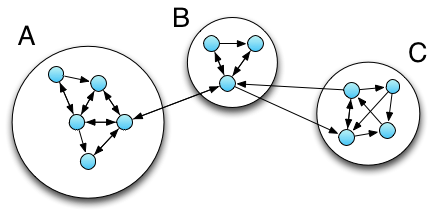
\includegraphics[scale=0.7]{2.Background/Media/communities.png} 
\caption{A hypothetical group of user communities}
\label{fig:communities}
\end{figure}

In more dense communities, Tweets can be made available to many users immediately after they are published, since many of the links between users are shared. This means that any retweets that occur within communities are likely to have a lot of \textit{redundancy}, in that many of the retweets will be sent to users who have already seen the Tweet. Although Twitter prevents this information duplication by not showing the retweets of Tweets that have already appeared on a user's timeline, it does increase the chance of the Tweet making its way out of the community.

Retweets amongst users within a community are likely to be common, due to the shared-interest nature of communities, and some users can provide `bridges' by being active in more than one community. In these cases, Tweets can be passed between the communities through retweets by the bridging user. If there are many users sharing communities, then there are many more avenues available for propagation to occur down, causing a high level of information throughput. If there are fewer bridges, then there is more of a bottleneck between the communities, hindering the information spread.

\cite{java07} also finds that communities can be formed from different types of people, such as those who Tweet frequently and have many followers, and those who contribute very little and have few followers. Those with many followers and many friends receive lots of information and have the potential to spread information further than those with fewer inward and outward edges. Studies in the behaviour of different types of users in Twitter is done more thoroughly in \cite{krishnamurthy08}, which defines `broadcasters' (users with many followers and few friends) and `miscreants' (users with few followers but many friends) and their roles in information propagation.

Users that retweet the interesting information from a source user to others, who do not follow the source user and so would not naturally receive the information, are effectively acting as information \textit{filters}. By not following the source user, a person might still receive the interesting information through these filters, but will not receive any of the `noise'. Thus retweeting means that friends of a user become useful filters of information for users further `downstream'  and retweeted information can be said to have a higher \textit{credibility} than Tweets that aren't retweeted \cite{castillo11}.


\subsection{User Influence}
Just as there are different types of user \textit{behaviours} on Twitter, as mentioned in the previous section, the are also users of different \textit{influence} levels \cite{quercia11}.

Much research has gone into user influence, including on how this might be detected \cite{yu11}, and influential users are generally found to be those that have a greater impact on Twitter's social network \cite{bakshy11} and that usually have significantly more followers than an average user. Influential users tend to have a high persuasion over other users, relating \textit{influtentials} in Twitter to those who are also influential in the real world as part of traditional communication theory \cite{cha10}, and therefore many Twitter influentials are the accounts belonging to real-world celebrities.

As with real-world celebrities, Twitter influentials are those with many `influenced' followers, or fans, which are the users who have the strongest agreeable opinions of the influential. As a result, an influential user has a greater number of followers who are interested in the information produced by the user, and is therefore more likely to receive more retweets than less influential users.

Although influence level is partly derived from the follower count of the user, it should be noted that a user with high in-degree on the social graph\footnote{In-degree: many followers} does not necessarily imply a high level of influence. An `active' audience of users who reply, retweet, and interact are more indicative of an influential user \cite{bigonha10}. This is especially true since a user can gain more followers through campaigns such as `\#teamfollowback'\footnote{Users associate themselves with \#teamfollowback to imply they will return all followships.} or by following `out of politeness', in which a user will follow another user back as an act of politeness, but these users tend to have \textit{both} high in- and out-degree and invoke less interactivity amongst their followers, which are not necessarily characteristics of an influential user \cite{cha10}.

Klout\footnote{http://klout.com} is a web service that attempts to review a user's social media influence by assigning users a Klout Score. Their website declares that this score, which ranges from 0 to a maximum of 100 and whose generation algorithm is kept private and unpublished \cite{edwards13}, is determined from a variety of 400 sources taken from eight different social media platforms, and which \textit{also} seems to take interactivity between users as the primary indicator \cite{anger11}. Additionally, the service indicates the topics a user is influential about, with the general idea being for organisations to check up on which users are influential for marketing purposes, but also to highlight the users that should be replied-to at a higher priority.


\subsection{Twitter as an Information Retrieval System}
From a high level, Twitter is essentially just a variety of information-retrieval system, which people can utilise to produce and consume information when required. In traditional information-retrieval systems, such as search engines and library systems, keywords and search terms are common ways for describing the type of information the user would like to receive back. The system would then search a database or archive for what it believes is relevant information, \textit{based} on these `retrieval parameters', and return results to the user ordered usually by the estimated relevance of the articles \cite{arvola10}.

Information quality is also reliant on the expected reading effort of the returned documents. The character precision-recall metric was introduced by \cite{arvola10} by way of demonstrating the tolerance-to-irrelevance ratio. The general mechanism for this ratio is to do with users reading a document passage; the point at which this ratio is reached is when the user stops reading the particular passage and moves to the next whole document, since they assume the rest of the document is also irrelevant to them.

Therefore, the more effective the information retrieval system is in displaying high-quality information, the lower the chance that this ratio is reached by the user.\\ 
It is comparable that a Twitter user viewing Tweets from a user they are following may get to the point where he or she reaches this ratio (i.e. is beginning to get bored or find the Tweets irrelevant) and decides to unfollow the friend. Similarly, the more effective the user is when selecting people to follow in the hope of receiving interesting information, the less likely it is that the user will remove these friends.

Whilst Twitter does not support the use of keyword searching for its primary information delivery method, it does lend its users some control over the type of information they wish to receive. As mentioned previously, users receive all of the Tweets from everyone that they follow onto their home timelines. Thus, by selecting users to follow, a person is effectively describing and implicitly indicating the type of information he/she would like to receive, and by editing their friends list (either by adding new followers or pruning existing ones) he/she can alter this indication.

Despite this control, it is still unlikely that users will achieve a perfect Twitter experience due to the presence of \textit{noise} \cite{alonso10}. As discussed in the Introduction, this problem stems from that although a person follows users they consider to be interesting, it is often the case that not \textit{all} information produced by interesting users will be interesting itself.


\subsection{Information Quality, Popularity and `Interestingness'}
Information-retrieval systems typically use some measure of information \textit{quality} when determining which documents to return to a user and also when deciding on the \textit{order} the documents should be displayed in. This `quality' is subjective in that different systems use a variety of different algorithms for deducing quality, usually based on the level of \textit{interest} in each of the available documents (such as Google's Page Rank algorithm and Amazon's recommendation algorithms), but also in that the level of quality itself depends on the user itself requesting the information. 

In the case of Google's Page-Rank, the algorithm uses multiple cues to determine who the user is, their interests, past searching habits, links clicked, and so on, to return \textit{relevant} information, which is incidentally one of the causes of the aforementioned Google search bubble.\\
Amazon's recommendation algorithms analyse a user's past item views and purchases and cross-matches these against trends based from users who also looked or bought similar items. Amazon is then able to accurately determine the type of items a customer are interested in purchasing, and can send emails to that customer with personalised recommendations.

Thus, information quality is essentially a function of information interestingness and information relevance, which are both related to the concept of \textit{effective stimulation} \cite{xu07} discussed later.

Twitter uses no such metrics to deliver information to its users, relying on the users themselves to implicitly `choose' the information they want to receive - it is an information retrieval system and not a recommendation system. Additionally, information is always displayed in chronologically-ordered timelines, with new Tweets being continuously inserted at the top as they occur. Twitter does not try to indicate interesting Tweets on the timeline which means that the interesting information is shown at equal value alongside the `noisy' Tweets, causing the difficulties in identifying the interesting information as has been mentioned previously.\\
Indeed, the recent TechCrunch article from October 2013, ``Twitter Quitters And The Unfiltered Feed Problem''\footnote{http://techcrunch.com/2013/10/05/sorry-my-feed-is-full} talks at more length about this particular phenomenon, and helps highlight the problem area of this work more clearly.

The retweet count of a given Tweet is a useful metric in inferring a Tweet's \textit{popularity}. If a Tweet is retweeted 10 times, then ten people have taken the time to read that Tweet, decide it is worth sharing, and then actually retweet it \cite{uysal11}. This user (and the other nine retweeters) may have found the Tweet interesting, yet it should be noted that although the count can be used as a measure of popularity, as a function of the influence of the Tweet's author, the retweet count alone cannot be used as a measure of how interesting the Tweet actually is \cite{naveed11}. For example, it is inappropriate to say that the first Tweet in Figure \ref{fig:tweet_comparison} is so significantly more \textit{interesting} than the second, although it is clearly more popular since Justin Bieber is an extremely influential Twitter user.\\

\begin{figure}[h]
\centering

\includegraphics[scale=0.55]{2.Background/Media/compared_tweets.png} 
\caption{Example of Tweets with significantly different retweet counts}
\label{fig:tweet_comparison}
\end{figure}

Whilst the work in this thesis does not aim to build an accurate retweet-predictor, this does become a basis for some of the work in later chapters.\\
\cite{uysal11} identifies the same problem of `noisy' Twitter timelines and discusses methods for predicting \textit{popular} Tweets using a J48 decision tree classifier, based on the likelihood of the Tweet being retweeted by a particular user. Although the authors address information relevance from a user-centric point of view, the validations of whether a prediction of a retweet occurring for a given Tweet is actually indicative of the \textit{interestingness} of said Tweet do not perform particularly well.\\
A retweet-prediction model based on a factor graph model is introduced by \cite{yang10} to determine how retweetable a Tweet is on a global scale. A precision of just under 29\% is achieved in predicting if a Tweet will be retweeted, but no mention is made of how this relates to how \textit{interesting} the information is.\\
Another study into retweet prediction was carried out by \cite{zaman10}, in which a trained probabilistic collaborative filter model (named `Matchbox') was used to determine the useful features in making the predictions. As with the previous study, the research focuses on a retweet \textit{probability}, which is a binary decision made by one particular user. The methodology is not aimed at the inference of interestingness, and simply determines that the most relevant features for accurate decision predictions are the author of the original Tweet and the retweeter.

Inversely, \cite{suh10} and \cite{hong11} predict the \textit{type} of messages that are likely to be retweeted further, the latter using a logistic regression to both predict an individual retweet decision and a retweet \textit{volume}. The methods do not apply these notions to how interesting the information actually is, achieve low recall and the multi-classifications seems only to perform well on very unpopular or very popular Tweets. It is made clear, however, that the retweet volume of a Tweet is useful in denoting Tweet \textit{popularity}.

\cite{petrovic11} uses a passive-aggressive machine-learning algorithm to make binary predictions on retweet decisions and cited that social features - for example, number of followers of the author, frequency of Tweeting, etc. - were the largest factors in the performance, and \cite{naveed11} uses a logistic regression, partly using a dataset published as part of another paper by the same authors as \cite{petrovic11}, to predict retweet decisions in order to address information interestingness. However, little effort is made to define interestingness or, indeed, validate that the inferences towards this are accurate and correct.\\
A logistic regression is again used by \cite{zhu11} for predicting binary retweet behaviours with the focus on information propagation in disaster scenarios, and \cite{peng11} showed that conditional random fields can perform better than logistic regressions than when modelling retweet behaviour in the same way.

Since the above papers only effectively consider a prediction of retweet outcome, which is a binary decision, it is hard to relate this to more of a global interestingness, aside from stating that a retweet implies the retweeter's relative interest in the Tweet. However, a retweet count, as mentioned above, is inappropriate as an indicator of \textit{magnitude} of interest, and so the research into predicting individual retweet decisions cannot be used as a basis for this. Additionally, not much emphasis is placed on how well the techniques work `on-the-fly'; many of the methodologies discussed require several features that may take a long time to collect and compute, making them unsuitable for use as part of quick and useful interestingness evaluations.

The idea of Tweet scoring and retweet \textit{count} predictions is introduced by \cite{gransee12}, who used their methodologies to produce a system\footnote{https://sites.google.com/site/learningtweetvalue/home} enabling users to compile Tweets in ways that are predicted to achieve the most retweets. The predictions are based on averaging the score, derived through a linear regression, of different components of a user's Tweets (such as the inclusion of a particular hashtag), so that when a Tweet by the same author is next constructed, the various components of the new Tweet can be compared against the scores of the counterparts seen in previous Tweets. The value produced through this method is then used to generate an expected retweet count as part of a comparison to the user's average (`baseline') achieved retweet count at this point in time, and was shown to perform well on influential Twitter users.

However, the methods described do not take into account fluctuations in the social graph, particularly in the case of less-influential Twitter users, who's local networks are prone to more frequent changes. Additionally, they rely on enough previous Tweet and temporal information on the user to be evaluated, and do not relate the resultant score to any type of interestingness metric in the context of highlighting it from amongst noise.

Alonso et al. (\cite{alonso10}) also use `scoring' to address interestingness, focusing more on determining \textit{uninteresting} content, by assigning Tweets an integer score out of five. Although the authors initially attempted to train a decision tree classifier on a set of 14 features, they settled on classifying a Tweet as `possibly interesting' if it simply contains a URL, and otherwise classify it as `not interesting'. Although the authors did then further classify the possibly interesting Tweets, by studying the magnitude of the crowdsourcees used to evaluate the Tweets that found them interesting, and then classifying Tweets based on them containing a particular type of named entity - for example, a person's name, a place or brand name, and so on - the categorisation system is too coarse and is not capable of representing the many different types of Tweets seen on Twitter.\\
Additionally, despite achieving relatively high accuracy in this particular area, the methods are not suitable for assessing Tweets on a general or user-specific level, especially since Tweets that don't contain URLs might still contain interesting content.

An interesting study is described by \cite{lauw10}, in which a clustering algorithm is used, taking into account the retweet count of a Tweet and how this is related to the popularity of the source user, to determine information quality. Although this work is more similar to the research discussed later in this thesis than others, the scoring is quite simple and the author's use-case seems limited to that of identifying the most important Tweets surrounding a particular event (such as the death of Michael Jackson).\\
Additionally, the authors do not make any effort to verify their results in any way, aside from comparing the Tweets determined to have a high quality by each of their two assessed methodologies.


\subsection{Precision and Recall}
Precision and recall are two metrics that are often used simultaneously to verify the performance of a method or procedure, with the usual goal being to maximise both. The metrics are used for validating \textit{accuracy} in different ways, yet they can be applied to other purposes also and are useful in describing the notion of interestingness in Twitter.

The precision and recall measures are talked about somewhat in Twitter- and retweet-based literature. These pieces tend to only analyse the measures on their own work when applied to Twitter rather than on any more global scale. Certainly, there is less in the literature on the subjects of precision and recall with regards to retweeting in general.

The idea of assessing the credibility of information is introduced in \cite{castillo11}, in which the authors demonstrate methods of measuring the credibility of `news' and `chat' Tweets. In this case, retweeting is seen as a possible measure of a Tweet's credibility, since users typically only retweet information they see as interesting or useful. The authors use a logistic regression on a set of features derived from each Tweet in order to classify its credibility. 

The precision and recall metrics are used to verify the different aspects of the paper's results. In particular, they are applied to the classification of assessing credible information (and users) in order to calculate how well classified the information is. A higher precision, therefore, shows that their model has accurately classified most of the total information classified as either credible or non-credible.
\[	
	Precision = \frac{\text{Number of correct classifications}}{\text{Number of total classifications made}}
\]

\[
	Recall = \frac{\text{Number of correct classifications}}{\text{Total number of potential classifications}}
\]

On a similar note, \cite{hong11} discusses the notions of precision and recall more generally. The authors discuss the problem regarding the balance of information received by Twitter users. Having too few friends reduces the number or interesting posts received (i.e. low recall); having too many friends may cause information overload and is likely to include a lot of noise (i.e. low precision). This issue is used, instead of to validate results,  as a basis for the work; predicting the Tweets that are most popular and will be retweeted the most.

In addition, precision and recall are used to compare the method to two other baselines; the TF-IDF score and \emph{Retweet Before}, which uses the fact that if a Tweet in the training data has been previously retweeted, then it's likely to be retweeted again. The two metrics are also used to compare results when certain features are removed from the classifier. For example, showing that without using a `user retweet' feature,
the precision and recall remain significantly higher than when removing other features, meaning that this feature does not contribute highly to the performance. \\
More specifically, precision and recall are used in a similar way to in \cite{castillo11}; except rather than looking at the number of classifications made, the authors use the number of predicted retweets.

\cite{bigonha10} discusses a proof of concept for detecting influential users in one of two categories; evangelists or detractors. Precision and recall, in this case, are used slightly differently:
\[	
	Precision = \frac{\text{Number of influential users retrieved}}{\text{Number of users retrieved}}
\]

\[
	Recall = \frac{\text{Number of influential users retrieved}}{\text{Total number of users}}
\]

The concept is taken further through the use of another metric, the \emph{Mean Average Precision}, which is used to denote an influential user as being a detractor or an evangelist. \\
A high precision, in this case, would imply a large proportion of influential users are classified correctly and a high recall means that most of the influential users existing in the entire dataset have been classified. The final results then show the precision and recall values for detecting evangelists and detractors in both follower/following networks and interaction networks. Both precision and recall improved when the size of the set of highest classified influentials increased (i.e. the top set of influential users).

\cite{pak10} presents a method for the automatic classification of Twitter information to determine if a document is positive, negative or neutral in sentiment. In this case, the authors replace precision with \emph{accuracy} and recall with \emph{decision}, since they are using many classes instead of a binary classification, and define them as the following:
\[	
	Accuracy = \frac{\text{Number of correct classifications}}{\text{Number of all classifications}}
\]

\[
	Decision = \frac{\text{Number of retrieved documents}}{\text{Number of all documents}}
\]

The accuracy is measured across the classifier's decision, and the $ F_{0.5}-measure $  is then calculated based on these values instead in order to show that the classifier works well when the dataset size is increased.

As well as a good news source, Twitter is also used as an informational, user-contributed source on world events. \cite{marcus11}  introduces a system, TwitInfo, which can be used for detecting, summarising and visualising events from Tweets. The authors looked at football match footage, web content, and earthquake survey data, and manually annotated major events in each to produce ground truth sets. These would be use to compare and contrast the results produced by their event detector using the following definitions of precision and recall:
\[	
	Precision = \frac{\text{Number of events detected were from ground truth set}}{\text{Total number of events}}
\]

\[
	Recall = \frac{\text{Number of events detected}}{\text{Number of events in ground truth set}}
\]

With these definitions set, the authors were then able to easily calculate precision and recall for their algorithm.

For the work in this thesis, interestingness of information is the performance metric used to describe information quality, and thus precision and recall for any particular user in the scope of this thesis can be defined as follows:
\[
	Precision = \frac{\text{Number of interesting Tweets received}}{\text{Total number of Tweets received}}
\]

\[
	Recall = \frac{\text{Number of interesting Tweets received}}{\text{Total number of all interesting Tweets}}
\]
where \textit{received} means that the Tweet has arrived on the user's home timeline, but does not imply that the user has \textit{read} the Tweet.

Therefore, a user following many other users will receive lots of interesting information onto their home timeline in amongst lots of noise; resulting in a reduced precision and higher recall. Another user might follow a very select few other users who are of direct interest, and thus will experience high precision, but low recall.\\
These metrics are therefore useful in describing the concepts of noise and interestingness, and are consistent with their respective definitions in that users will achieve an optimum Twitter experience if both precision and recall are maximised.

Zadeh et al. (\cite{zadeh13}) defined bespoke definitions of precision and recall, yet also in the domain of interesting information on Twitter. Although the authors identify the need for users to be able to discover other users of interest and declare that Twitter does, in fact, have a `high precision' of interesting information, they admit to using a very coarse set of possible interest categories and is only based on \textit{overlapping} interests rather than addressing the interest-noise ratio more concerning the research in this thesis. Additionally, clicks on URLs by users are the only means by which to measure this interestingness, and Tweets with URLs are usually the most interesting type of information \cite{alonso10}.

\section{Collecting Twitter Data}
Most of the analytical work in this thesis relies on various data being collected from Twitter. Twitter provides an API for developers in order to facilitate the production of applications for its platform, but also for research purposes. It permits interfacing with many components of Twitter's service, such as posting and retrieving Tweets, interacting with other users (e.g. creating new friendships), and most of the features that Twitter's service itself provides to its users.\\
The API encourages use of the OAuth\footnote{http://oauth.net} authorisation framework to handle access\footnote{https://dev.twitter.com/docs/auth}, allowing Twitter to keep track of applications and each application's access privileges and rate limits\footnote{https://dev.twitter.com/docs/rate-limiting/1.1}.

Twitter's traditional REST API, v1\footnote{https://dev.twitter.com/docs/api/1}, provided many useful endpoints for data collection and allowed each OAuth-authenticated application 350 hourly POST and GET requests\footnote{https://dev.twitter.com/docs/rate-limiting/1}.\\
In June 2013 Twitter officially deprecated v1 of its REST API, forcing use of its new v1.1 API\footnote{https://dev.twitter.com/blog/api-v1-retirement-date-extended-to-june-11}. The new version contains many of the same resources\footnote{https://dev.twitter.com/docs/api/1.1} as the original, but workarounds are required to get the results as some of the endpoint requests possible through v1. Additionally, new rate-limit policies were introduced, allowing more limited and controlled access to most of the available resources.

Since the work in this thesis was ongoing over this switch-over date, the initial work utilised API v1, and the latter work API v1.1, causing some changes to some of the data-collection methodologies as the thesis progresses. Descriptions of the data-collection in each relevant part of the thesis reflect this change, where appropriate.


\section{Research Motivation}
The motivation for the work in this thesis lies in the need to distinguish interesting information from noisy Tweets in Twitter, the latter of which is the problem area identified over the previous sections of this thesis.\\
It has been made clear that the retweet count of a Tweet cannot reliably be used as a measure of interestingness, especially in the context of influential users, who naturally achieve significantly more retweets than average users, but which does not imply that the information they produce is of a higher quality or interest level.

As a result, the retweet count alone cannot be useful in distinguishing interesting information from noise in a timeline of mixed Tweets from different users with different levels of influence - some further metric is required to make this distinction. 

This thesis covers the procedure and research behind a methodology that determines and ranks information on Twitter through inferences of interestingness that allows the more interesting information to be brought forward. 

\chapter{Understanding The Behaviour of Retweeting in Twitter}


Stuff to finish up in this section:
\begin{itemize}
\item Explain motivation for research in this particular area
\item Use this motivation to explain the purpose for this research as a basis for the work in the next few chapters
\item Explain how this chapter is the basis for research into Twitter's social structure in the next chapter
\item Normalise terms (retweet-group size / retweet volume) here and in further chapters throughout thesis
\item (thinking forward: e.g. we have addressed tweet quality in terms of propagation, can a network have a quality too? what further factors can affect the dissemination of information in social networks?
\end{itemize}

It has been discussed that the popularity of information in Twitter can be related to the propagation characteristics of that information through Twitter's social structure. That is to say, that the more times a Tweet is retweeted by users, the more people have found the information contained within it to be interesting enough to be worth sharing.\\
It has also been shown that this retweet count metric alone cannot be an implication of the actual interestingness level of a Tweet. This is related to the notion of user influence, which directs that some tweets are naturally immediately seen by more people and thus have a higher chance of achieving a retweet as they are. Indeed, since follower count is one of the \cite{suh10} demonstrated that a user's Tweets' retweet rates increase as the user's follower count increases.

The strength of Twitter lies is in its social structure, where users can elect to follow and unfollow others as they choose. Followers of a user receive all of that user's posts in their individual (or `home') timelines. If a user has set their profile to be public, then their posts also used to appear on the public timeline, which is now deprecated but was accessible to anyone; even those without a Twitter account. As a result, people are likely to follow users who update with interesting posts; whether the follower is a big fan of the user and simply wants to know everything going on in their life, or if the follower is simply interested in the topical area of most of the friend's posts. 

Just as Twitter users will post Tweet about topics that are of interest them - possibly related to a user's work, a hobby, or a mixture of multiple areas - and these Tweets are generally posted with the idea that they will be useful or interesting for some of their followers as well as an attempt to attract more followers, retweets are generated with the same motives in mind. This means that if a Tweet is retweeted, it is not only allowed to disseminate further through the social structure, but also that a higher Tweet quality is implied.

Thus, this describes how a user's friends, who carry out retweets, effectively become filters of interesting information for that user and other followers of those friends, and the \textit{audience} of the original Tweet is significantly increased. Since retweets are always attributed to the original author then you, a Twitter user, may gain more attention by means of followers by posting \textit{interesting} Tweets, which will; 
\begin{enumerate}
\item increase the chances that users reading your Tweets will choose to follow you, and
\item increase the chances that users will decide to retweet your Tweet, thus broadcasting it to a larger audience. People viewing this \textit{retweet} then may decide to follow you. 
\end{enumerate}

Since a Tweet can be retweeted multiple times, and, as mentioned, a retweet itself can also be retweeted, the much larger the effective audience (both directly and through retweets) of a Tweet's original author has the potential to become if they choose to post interesting information. In this chapter, an understanding of the behaviours and properties of retweets is provided, along with discussions into how these are relevant in determining useful metrics for determining which retweeted information is interesting.


\section{Tweet and Retweet Properties}

\subsection{Retweet Groups}
A Tweet has various attributes associated with it, which make up the features that describe that particular Tweet. Each Tweet has a set of properties relating to its content, its author, and other metadata, such as creation time.\\
As such, a particular Tweet, $t$, can have its relevant properties declared and be defined as follows;
\[
	t = (\mathrm{text}, \mathrm{count}_R, \mathrm{author}_O, \mathrm{author}_R, \mathrm{orig})
\]

Respectively, this represents the Tweet's text, its retweet count, and the \textit{original} author of the Tweet. The final two values depend on whether $t$ is a retweet or not and represent the author of the retweet and the original Tweet respectively. Since a retweet remains a class of Tweet, then the same properties can be assigned to retweets as to Tweets, except that in the case of retweets the values $\mathrm{orig}$ and $\mathrm{author}_R$ will be non-null.

Since a Tweet can be retweeted more than once, the set of Tweets that are in the set of \textit{all} Tweets, $T$, and are retweets of $t$ is defined as;
\[
	RT(t) = \left\{ s \in T : s.\textrm{orig} = t \right\}
\]

Clearly, the retweet count of $t$, $ t.\mathrm{count}_R = \left\vert{RT(t)}\right\vert $.

An original Tweet, $t$, along with all of the retweets of $t$, $RT(t)$, are known as the \textit{retweet group} of $t$, which is defined as $G(t)$ and is useful when discussing the audience reach of a particular Tweet. Therefore, since $t$ is also a member of this set, the size of $t$'s retweet group is; 
\[
	\left\vert{G(t)}\right\vert = t.\mathrm{count}_R + 1 
\] 
If $ r_1,...,r_n $ are the members of $RT(t)$ then the raw audience size of the group can be calculated thus (assuming $t.\textrm{count}_R \geq 1$);
\[
	\textrm{audience}(G(t)) = \textrm{followers}(t.\textrm{author}_O) + \sum\limits_{i=1}^{t.\mathrm{count}_R} \textrm{followers}(r_i.\textrm{author}_O)
\]

However, properties of Twitter dictate that this raw audience size is not an accurate calculation in most cases, as is discussed later in this chapter.


\subsection{Retweet Trees}
As a Tweet gains in popularity and attracts more and more retweets to be created from it, and since retweets themselves can also be retweeted, then this ultimately results in the generation of a retweet \textit{tree}, which represents the retweet group of a particular Tweet. This tree is formed from the \textit{users} who have retweeted the Tweet (or a retweet of the Tweet), and represents the original Tweeter and the various pathways taken by the Tweet as it is retweeted through the social graph.

The tree is not a representation of the actual social ties between the tree's nodes, as users are able to retweet Tweets and retweets sent from others that they do not follow. However, as is mentioned later in this chapter, most retweeting does generally occur between directly-linked users.

The root of the tree representing every $G(t)$ is $t.\textrm{author}_O$ and, if $t$ has been retweeted, each of the other nodes are $$r_1.\textrm{author}_R, ... , r_n.\textrm{author}_R \: \forall \: 1 \leq n \leq t.\mathrm{count}_R $$\\
A similar illustrative device is used by \cite{galuba10} in describing URL \textit{cascades} in Twitter.

\begin{figure}[h]
\centering
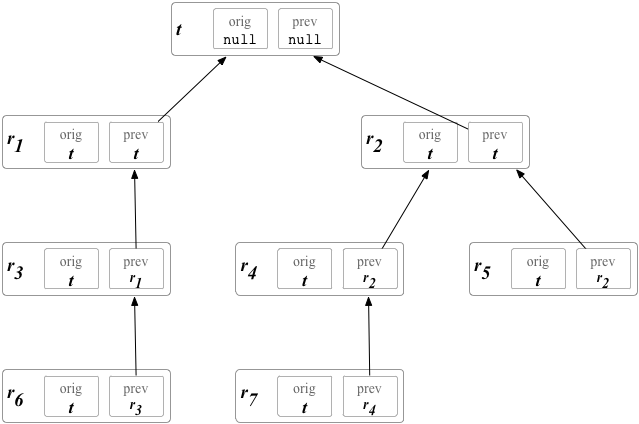
\includegraphics[scale=0.5]{3.Chapter1/Media/tree.png} 
\caption{\textit{A hypothetical retweet pathway tree.}}
\label{fig:retweet_tree}
\end{figure}

Although these retweet pathways can technically be acyclic through the use of the manual retweet method, the case of a user retweeting a Tweet more than once is very rare and a user retweeting a retweet that they are already part of the upstream chain of is even less likely to occur. The retweet button method simply does not support users retweeting a Tweet more than once.\\
As such, retweet trees are used in preference over retweet \textit{graphs} as they illustrate the temporal nature in terms of the order in which the retweets occur.


\subsection{Path-Length}
In addition to retweet groups having a size property, a retweet groups's branch's \textit{path-length} refers to the length of a particular retweet chain. In particular, it defines the number of times a Tweet is retweeted down one chain from the source user (the retweet group's tree's root) down to the final retweeter in the chain (a tree's leaf node).

Figure \ref{fig:retweet_tree} represents the users in the retweet group of a hypothetical Tweet.\\
This retweet group has a size of 11 and has 7 distinct retweet chains, the longest of which is the one traversing users 1, 3, 6 and 11.\\
The \textit{maximum} path-length of this retweet group is therefore 3, as the leaf node of this branch is three hops away from the original author at the root.

As has been mentioned previously, when a user retweets a Tweet or retweet through the manual approach, it involves pre-pending the current state of the Tweet with the text \texttt{RT @<username>:}.\\
Therefore, the Tweet with the content;\newline
\texttt{RT @user2: RT @user1: This is the body of the Tweet}\newline
was originally authored by \texttt{user1}, then retweeted by \texttt{user2}, and then finally retweeted by the author of this current retweet (the author of a Tweet or retweet's username is not credited in the body of the text).

It should be noted that this phenomenon can only be observed through retweets by the manual approach, since the button method always simply credits the original author, and not any of the internal members of the retweet group.

Although most retweets today are carried out using the button method, the manual approach still remained popular at the time the research in this chapter was carried out. This allowed for making useful observations of retweet patterns that would not be as prevalent later on.


\section{More on Information Retrieval}
A Twitter user electing to follow another user cannot predict precisely what the new friend will Tweet about in the future. The user has some \textit{expectation} of the type of information they are likely to receive based on the previous Tweets of the new friend, which is generally the only cue the user can use to base the follow decision on.

Part of the follow decision is based on the notion of relevance judgement, which is a notion discussed at more length by \cite{xu07} and is partly made up of the goal of achieving \textit{affective stimulation} through \textit{hedonic} searching as opposed to the use of \textit{epistemic} searching.

\subsection{Epistemic Search}
An epistemic information search is one that involves carrying out a search with the purpose of finding out information on a particular topic (or set of) to satisfy a \textit{desire for knowledge} \cite{xu10}, yet without an actual aim to solve any particular problem.

An example of this type of search is a `crawl' through Wikipedia, in which a searcher may start at one particular page of interest and then follow links within that page to other related pages of interest that stem away from the source topic. In this case, the search `parameter' is simply the name or title of the article the searcher wants to view.\\
As mentioned previously, a followship between users is effectively a search parameter in Twitter, since the following user has elected to follow the new friend to receive information from him/her. It is clear that this type of `searching' cannot be epistemic as the following user cannot know exactly the type of information they are going to receive.

\subsection{Hedonic Search and Affective Stimulation}
Hedonic searching is similar to epistemic searching in that it is also not carried out with the aim to solve an immediate problem, but is different in that it is done to search for fun or `affective stimulation' \cite{xu10}.

A person can be said to be affectively stimulated if they view a piece of information that has some effect on the person, such as an emotional effect, something that is of particular interest to the person, or something that is capable of provoking some further thought.

With hedonic searching, users are not aware of the information that they are going to receive prior to searching and thus cannot really predict any level of affective stimulation.\\
This aligns more with Twitter usage, since users receive information that they cannot accurately predict. Any Tweets received that do and provide interesting information convey affective stimulation to the user. This is the type of information that becomes harder to identify amongst lots of noise, yet is also the type of information a user is more likely to retweet.

\subsection{The Recognition Heuristic} 
A further metric for measuring information relevance in information retrieval is the recognition heuristic.\\
The recognition heuristic takes advantage of a person's memory and declares that if a person is able to recognise only one of two (or more) items, then he/she is more likely to judge the recosnided item to be `greater' or more important \cite{oppenheimer03} \cite{goldstein99}.

Relating this to information received on Twitter, \cite{chorley12} found that a user recognising a Tweet's author significantly increases the chance that the user will decide to read the Tweet. Since a user must read a Tweet in order to make a decision on whether, or not, to retweet it, then the recognition heuristic transiently plays a part in a user's retweet decision also.

The authors also find that information about the Tweet itself, such as its text content and its retweet count, has much more of an effect on a user's read decision than information about the author, such as the followers count or Tweet rate. This also contributes to the declaration that information interest goes beyond the features surrounding a particular user and that user influence does not dictate interestingness of information.


\section{Twitter Analysis}


Discuss wanting to know more about Twitter and the way information is propagated through this. \\
Want to gain a base knowledge of some of the propagation patterns in terms of the tweets and the networks the tweets travel through. \\
This will form basis of research further on. \\ 
Stuff interested in:
\begin{itemize}
\item retweet groups (define)
\item path-length (define)
\item friend/follower graph 
\item timings, etc.
\end{itemize}

\section{Experimental Methods}
\label{experimental methods}
% take some of this and add to Twitter Analysis section (maybe will be renamed)
\subsection{Data Collection Methodology}
The experiments conducted involve the examination of tweets selected randomly from the Twitter public timeline\footnote{Viewable from \textit{http://www.twitter.com/} when not logged in.}. The system interfaces with the Twitter REST API and periodically retrieves the top 20 tweets from the timeline, filtering out the posts that are retweets. They are distinguishable as they start with the characters `RT' followed by a username. These retweets are then stored and the original tweet text is extracted. Sometimes retweets are made with additional text as comments, which made it harder to retrieve the actual original text. In these cases, additional queries are made to try and source the original text, but, failing that, the retweet is discarded.\\
The original text is then used to query all available tweets for the original tweet and any other retweets. The original tweet, along with its set of retweets is referred to as the \textit{retweet group}. As a result, each retweet group contains precisely one original tweet and at least one associated retweet, thus the smallest possible retweet group is of size two. The \textit{final retweeter} is the most recent person to retweet the post. Results are generated by extracting data from these retweet groups, which are stored with metadata such as time, source, language, and so on.\\
It should be noted that there are two ways in which tweets can be retweeted. The traditional (or \textit{old}) manner involved users copying the existing tweet (or retweet) from the timeline before tweeting that with the characters `RT' and the previous retweeters username at the start. This ensures that the appropriate users are cited as being the author of the tweet. The \textit{new} method enables users to retweet a post simply by clicking the `Retweet' button that is available next to the post on the timeline both on the main Twitter website and on various Twitter clients. Despite the fact that the website and clients have alternate ways of displaying these types of retweets, the search interfaces and API still see them as starting with `RT' and the previous poster's username. This, fortunately, means that both types of retweets can be collected in the same way. Retweeting in the latter method, however, is unavailable if the post that is to be retweeted belongs to a user who has a non-public profile.\\
Despite this, the new method doesn't have direct support for retweet chains (explained below) to be formed. No matter who retweeted the post previously (whether they were the original poster, or not), the new retweeting method simply treats it as a direct retweet from the original poster (as long as the previous retweets were also made in this fashion). The original tweet (and other retweets) can still be found using the search method outlined above, however, so this doesn't significantly affect results. Limitations with both the Twitter API and the search interfaces did mean that not all retweets could have successful queries made against them.\\
As briefly described above, these experiments use the notion that retweets themselves can be retweeted; analogous to routers forwarding packets in a multi-hop networking system.\\


\subsection{Data}
There are three sets of experiments detailed in the following section and all of the data was collected using the search method outlined above. The data consists of around 4400 retweet groups (representing a total of about 26,000 tweets and retweets) collected between 26th January \& 24th May 2011. It is acknowledged that this is a relatively small result set and so we emphasise that these are \textit{preliminary} experiments to provide insight into the decentralised side of Twitter and to act as a start point for future work in this area.\\

\section{Empirical Results}

\subsection{Length of Retweet Chains}
\label{length of retweet chains}
The longest path-length encountered from the dataset of retweet groups was 9, meaning that the tweet has been forwarded nine times from the original user; making the total number of involved users ten. Despite this, in the dataset, the average path-length was around 1.8, with the vast majority of tweets being retweeted between one and two times, as shown by the distribution in Figure \ref{fig:pathlength-distribution}. The \textit{maximum path-length} of a retweet group refers to the longest path-length present in the group.\\
\begin{figure}[h]
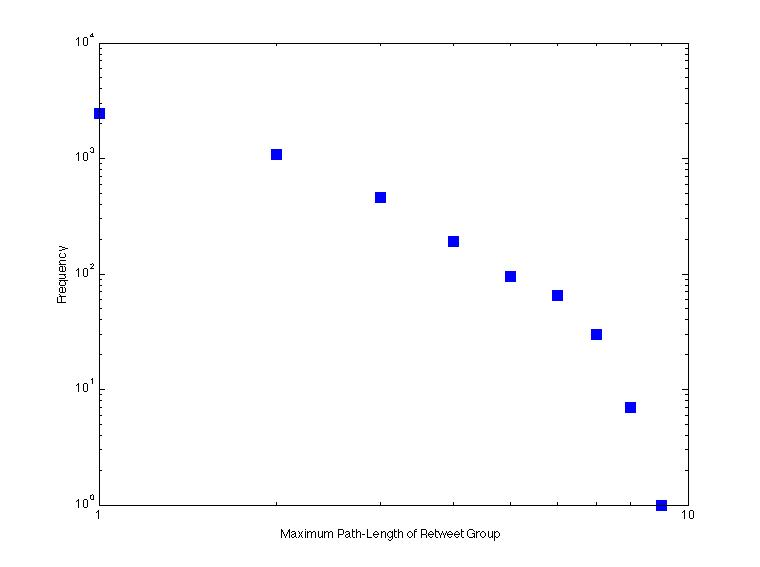
\includegraphics[scale=0.35]{3.Chapter1/Media/pathlength-distribution.jpg} 
\caption{\textit{Log/log distribution of maximum path-lengths from retweet groups.}}
\label{fig:pathlength-distribution}
\end{figure}
It should be noted that the very high proportion of single-chain path-lengths could be a result of the new method of retweeting introduced in the previous section, since, as mentioned, if all of the users in a retweet chain were to retweet in this way then Twitter would still only treat the path-length as one; between the original tweeter and each of the intermediate retweeters. Despite this, the result fits the rest of the dataset well.\\
This data can also be used to have a look at the friend-follower graph associated with retweets. In cases where the group's maximum path-length is equal to one (i.e. simply the case where a user has retweeted another user's tweet once), the retweeter follows the original tweeter about 90\% of the time. This implies that in 10\% of cases, a retweeting user has retweeted a tweet found outside of their home timeline, i.e. on the public timeline, or whilst browsing through other users. It could also be as a result of the retweeter not including the tweet citation (`@username') for reasons such as to save space, which would be particularly likely in cases of longer tweets. This implies that the more followers a user has, the greater chance that user has of having his or her tweets seen and of being retweeted. Since 90\% of retweets occur if the retweeting user follows the original tweeter, then this is directly demonstrated. However, this does not take into account whether the tweet was passed down a chain of retweets retweeted with the second (single click) method. In these cases the path-length would be represented with a length of one even if they were actually longer. The introduction of the second method of retweeting is, therefore, not helpful with the analysis of retweets.\\
In addition to this, in cases where the maximum path-length is greater than one (i.e. at least one user retweeting in a chain between original tweeter and final retweeter), the final retweeter follows the original tweeter in about 40\% of cases. From Figure \ref{fig:totalretweets-pathlength} we can see that retweet groups with a larger maximum path-length tend to be larger themselves. This means that the tweet has travelled further both around the original tweeter, but also potentially to other communities. Users from other communities will be less likely to follow this original tweeter, explaining this drop in likelihood. Results have also hinted that the probability of users citing the original tweeter decreases as the path-length of the retweet increases, which also goes some way to explain this point. 

\subsection{Size of Retweet Groups}
\label{size of retweet groups}
This section focuses on properties of retweet group size, and also how this can be related to path-length. The average retweet group size found from the data was of size 6, with the largest and smallest retweet groups being of size 284 and 2 respectively.\\

The distribution of retweet group sizes can be seen in Figure \ref{fig:retweet-distribution} and shows that this data follows a power-law distribution (with a relatively large \textit{p}-value of 0.871). The $Pr(X \geq x)$ represents the complementary cumulative distribution function, where the randomly generated \textit{X} is greater than or equal to \textit{x}. These values were calculated using the techniques and code provided by \cite{clauset07}.\\
In these retweet groups, and particularly the larger ones, retweets are likely to be down several chains. Combining this information with that of the average path-length of retweets, it becomes more clear how the retweet tree structure is created, with nodes being the retweeting users (the root node being the original tweeter), and edges between nodes being the path of retweets. Different retweet chains would be illustrated by the combinations of journeys down different branches. The longest path-length would be represented by the depth of the longest tree branch, and the total number of retweets would be represented by the number of edges. The trees can be said to represent the retweet groups, though, in practice, many members of the group will be separate from the main tree due to missing citations.\\
\cite{kwak10} discusses retweet trees in more detail, in particular, the different shapes of the trees representing retweet groups from the Air France incident. Their results, for these trees, also (see section \ref{length of retweet chains}) indicate a large number of groups with maximum path-lengths of one and two.\\
\begin{figure}[h]
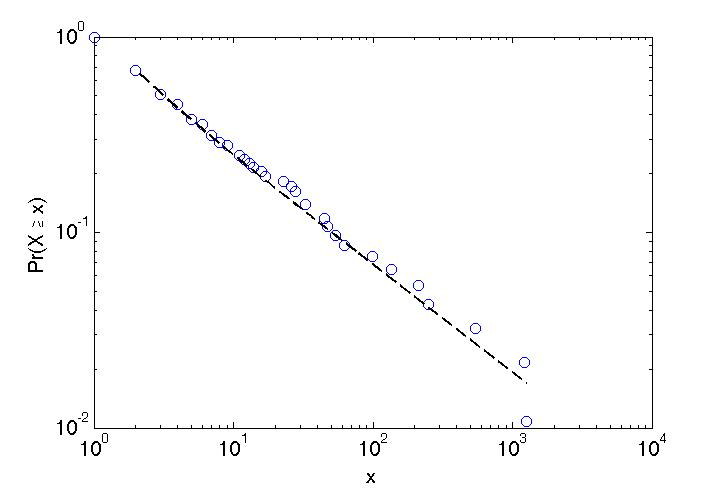
\includegraphics[scale=0.35]{3.Chapter1/Media/retweets-distribution-stats.jpg} 
\caption{\textit{Maximum likelihood power-law fit for the cumulative distribution of retweet group sizes.}}
\label{fig:retweet-distribution}
\end{figure}
\begin{figure}[h]
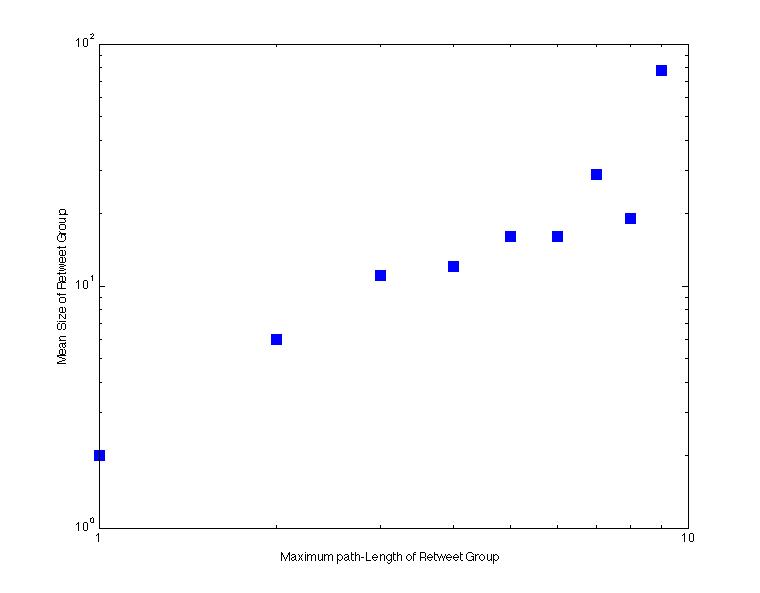
\includegraphics[scale=0.35]{3.Chapter1/Media/retweets-pathlength.jpg} 
\caption{\textit{Log/log relationship between the maximum path-length and size of a retweet group.}}
\label{fig:totalretweets-pathlength}
\end{figure}
Figure \ref{fig:totalretweets-pathlength} shows how the total number of retweets varies with the longest path-length of the retweet group. The trend mostly correlates with what might be expected; that the maximum path-length of a group increases with the overall size of the group. These illustrations do not show which users are followers of others, but do show how some tweets are retweeted significantly more than others. Users who have many more followers are said to be more \textit{influential}, say Cha M. et al. \cite{cha10}, who also discuss the idea of `indegree', and that those users who have far more followers than friends are likely to be far more influential. Their chance of having tweets retweeted is therefore increased.\\
The (immediate) audience size of a retweet group refers to the number of users the tweet has been exposed to either directly or through retweets. \textit{Immediate} was used in this sense since users who have made their profile public can have their tweets viewed by users who aren't followers of the former. This audience size can therefore be calculated simply by summing up all the followers of each of the users in the retweet group.\\
\begin{figure}[h]
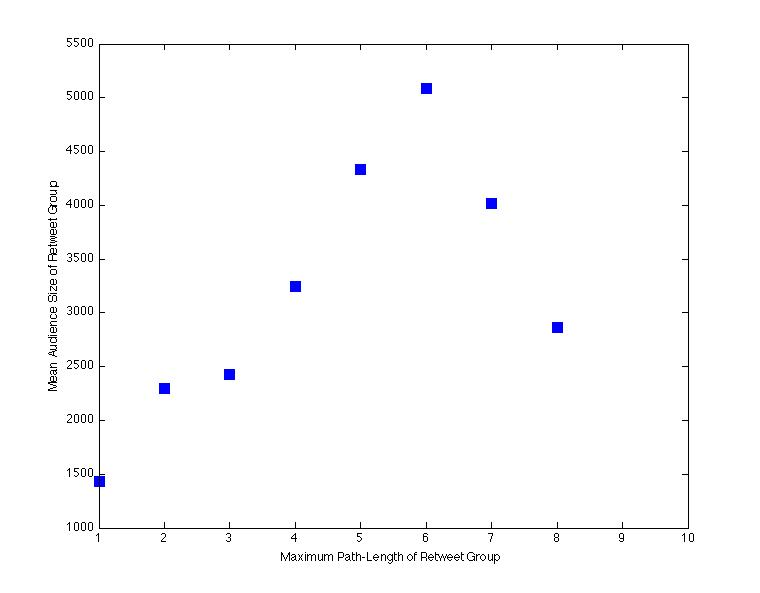
\includegraphics[scale=0.35]{3.Chapter1/Media/audience-pathlength.jpg} 
\caption{\textit{Relationship between a retweet group's audience size and its longest path-length.}}
\label{fig:pathlength-audience}
\end{figure}
These audience measures take into account that some users may be exposed to the same tweet more than once. This happens when users involved in a retweet tree have some followers in common, and so is likely to be prevalent in more closely-knit communities. As a result, the audience sizes shown only represent \textit{distinct} users exposed to the tweet.\\
Collection of the audience size from the data started slightly later than the main dataset and is only available for 2860 of the total 4400 groups. The longest maximum path-length of this subset is 8.\\
Figure \ref{fig:pathlength-audience} shows how the audience size of retweet groups varies with their maximum path-length. The peak at path-length 5 indicates that the groups with a mid-range maximum path-length tend to have a larger audience size, and we believe this is to do with the amount of audience overlap in different retweet groups.\\
\cite{kwak10} discusses how retweeting is related to the audience size of a tweet and how the power of the retweet phenomenon can greatly affect the spread of information, even if the original tweeter has only a few followers. The same paper more specifically mentions that the audience size of a retweeted tweet reaches, on average, at least 1,000 users, no matter the number of followers of the original tweeter. This can also be seen in our results; that no matter the maximum path-length of a tweet, the number of users reached is relatively high.\\
The overhead of a retweet group represents the number of users who are exposed to a tweet more than once and is present in 71\% of retweet groups. The \textit{proportionate} overhead is the ratio of overhead to audience size and the mean of this was found to increase with the group's maximum path-length. This is a possible explanation for the peak in the data: that eventually the overhead of non-distinct users has increased to the extent that it reduces the audience size more significantly. The same graph representing the effective audience size (calculated with the addition of non-distinct users) represents, mostly, a continuous positive correlation.\\
Three of the largest five overheads collected were from retweet groups with a maximum path-length of 1, the largest with an overhead of 6.5 times greater than the distinct audience itself (the overhead was larger than the actual audience size in around 3\% of retweet groups). This shows that, to an extent, there can be significantly more overlap in more closely-knit communities; those retweet trees which are wide and shallow. The chance of getting no overhead increases in smaller retweet groups.

\subsection{Retweet Follower Pattern}
\label{retweet follower pattern}
This experiment focuses on the pattern of followers in the retweeting hierarchy.\\
The first result shown from the experiment is that the final retweeter follows the previous retweeter in the chain in 67\% of cases. It initially seems strange that this should be 20\% lower than when following a user in retweet chains of length one. This suggests that users involved in shorter-chain path-length retweets are members of more tightly-knit communities. Retweets with longer path-lengths have, by nature, travelled further and so would be the type of retweet to travel between communities, reducing the chance of the involved users following each other.\\
The interesting part of this, however, is the number of followers of the previous retweeter in different cases. In the 33\% of cases where the final retweeter doesn't follow the previous retweeter, the latter has, on average, around 600 followers. When the final retweeter \textit{does} follow the previous retweeter, however, the previous retweeter's average number of followers is 940. This is quite a substantial difference and certainly highlights the fact that by having more followers you are more likely to have more influence in terms of whether you get retweeted, or not.\\
This is accentuated further when looking at the original tweeter. The likelihood of a retweeter following the original tweeter in cases in which the path-length is of more than one has already been found to be around 40\%, but the average number of followers of the original tweeter increases by a factor of around four (580 to 2000) when also followed by the final retweeter. Results showed that the original tweeter had a consistently higher number of followers when followed by the final retweeter than when not at all path-lengths. This demonstrates that having an increased number of followers is correlated with the chance of a user being retweeted. In this case, having four times the followers increases the correlation dramatically (40\% to 90\%). The number of followers of a user can therefore be directly related to the ideas of influence discussed in \cite{cha10} and also of `advertising' themselves.\\
\begin{figure}[h]
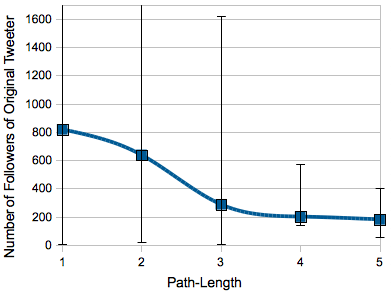
\includegraphics[scale=0.6]{3.Chapter1/Media/originalfollowers-pathlength-distribution.png} 
\caption{\textit{Relationship between number of followers (and respective distribution) of the original tweeter as the path-length increases.}}
\label{fig:originalfollowers-pathlength}
\end{figure}
It was found, however, that the number of followers of the original tweeter diminishes as the path-length of the tweet increases (Figure \ref{fig:originalfollowers-pathlength}), signifying that tweets travel further when the original tweeter has fewer followers. Because the retweet groups were collected in such a way so that groups containing longer path-length retweets also contained many shorter-chain retweets, retweet groups containing path-lengths of 5 (or more) are also likely to contain many retweets (if not more) with path-lengths of one or two (see the distribution in Figure \ref{fig:pathlength-distribution}). It can therefore be argued that there are more users involved in shorter-chain retweets than in ones with longer path-lengths. It is then more likely for these users to have more followers than others in the retweet group. Another explanation could be that users are actually aware of their local network and realise that retweeting may cause a lot of audience overlap (particularly in the case of large communities). A user may have seen a post retweeted a few times on their home timeline and thus decide not to also retweet.\\
One last interesting point to make regarding the notion of retweet chains is looking at the how the pattern of following previous retweeters develops as the path-length increases. It has already been discussed above how the chance of following the previous retweeter in the chain is about 67\%, but, in cases where the path-length of a tweet is greater than two (i.e. at least two intermediate retweeters between final retweeter and original tweeter), the chance of the final retweeter following the next retweeter along preceding the previous retweeter is around 45\%. This suggests that retweeting is more widespread and not so much just circulated around communities. These preliminary results demonstrate that the chance of the final retweeter following previous retweeters - up to and including the original tweeter - diminishes along the chain or as the tree is ascended (Figure \ref{fig:following-possibility}).\\
\begin{figure}[h]
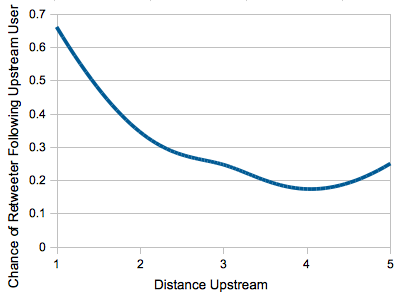
\includegraphics[scale=0.55]{3.Chapter1/Media/following-possibility.png} 
\caption{\textit{Proportion of final retweeters following upstream users at varying distances along the chain.}}
\label{fig:following-possibility}
\end{figure}
Because of this, it's sensible to assume that the tweets in the dataset are forwarded through less-connected users, and perhaps forwarded from community to community by those users belonging to several groups. Otherwise, if the retweets were circulated more around closely-knit communities, the likelihood of the final retweeter following the previous tweeters would be both greater and more evenly spread - i.e. the chance of following the previous retweeter would be roughly equal to the chance of following the other tweeters in the chain.\\
In addition, of the 67\% of final retweeters who \textit{are} following the previous retweeter, about 19\% of them also follow the next previous retweeter (i.e. the retweeter at path-length - 2). In this case, the next previous retweeter has, on average, 3000 followers. In the 81\% of these users \textit{not} following the next previous retweeter, then the latter has an average of 525 followers. This is an accentuated result of the one previously, but this time boasts an increase of a factor of 6.\\
Of the 33\% of users who \textit{don't} follow the previous retweeter, about 30\% follow the next previous retweeter. Both of these sets of statistics also go towards the idea of the diminishing chance of following the users as the tree is ascended.\\
From this dataset, it was also possible to work out how often retweeters cited the original tweeter of a post. In retweets, users are typically cited by, as we have seen, having their name along with an `RT' at the start of the post. This data was collected by seeing if the original poster's username was mentioned \textit{anywhere} in each retweet. The chance of this occurring was found to be around 68\% and did not vary with any pattern with path-length.
 
\subsection{Retweet Time Delay}
\label{retweet time delay}
The final experiments in this section focus on the time delay between the final retweeter and original tweeter. This is an interesting area since it enables researchers to see how fast messages propagate through the Twittersphere. From this information, and by using the retweeter patterns demonstrated above, it would be possible to work out how far and how quickly information can be passed around.\\
Figure \ref{fig:timedelay-pathlength} shows the average time delay between the first and final retweet with increasing maximum path-length of the retweet group.\\
\begin{figure}[h]
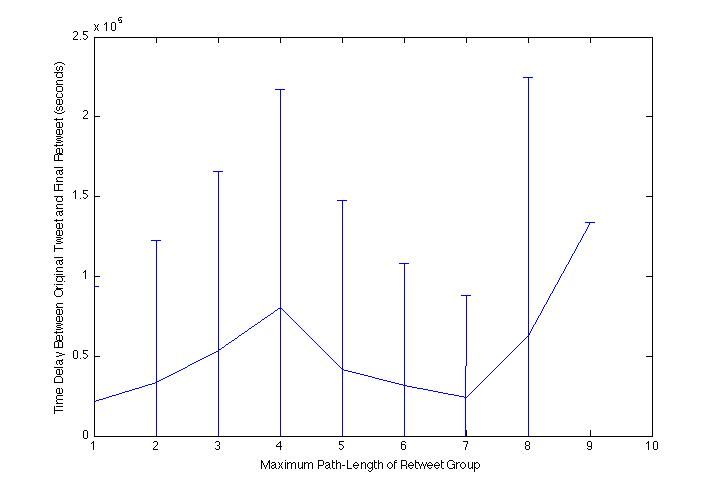
\includegraphics[scale=0.35]{3.Chapter1/Media/pathlength-timedelay.jpg} 
\caption{\textit{Average time (in seconds) between first post and final retweet of a retweet group varying with the group's maximum path-length.}}
\label{fig:timedelay-pathlength}
\end{figure}
The results indicate that, mostly, as the group's maximum path-length increases, then so does the elapsed time between the original post and the final retweet. This is probably as was expected, since this shows that it takes longer for a retweet to travel further. The data is not consistent, however, especially results for a path-length of five and above. The first four results suggest a uniform incline roughly proportional to $ v=\frac{s}{t} $, where the distance, \textit{s}, is the hypothetical distance given by the path-lengths, showing that the \textit{speed} of propagation remains mostly constant.\\
There is not enough of a trend in the data to make any deductions regarding propagation speed, however. There are two main conflicting arguments regarding this result: the first is, as mentioned, that the further a tweet travels the longer time it travels for. The second is to do with tweet popularity: the more popular a tweet is, the more quickly it will be retweeted. In the latter case, it is possible that longer trees grow fully before shorter ones, implying exponential growth. Generally, though, it seems that the maximum path-length of a retweet group does not massively affect the tweet's propagation speed.

\section{Summary}
\label{analysis}
The experimental results have certainly highlighted the ideas of communities and that of message cascading similar to that demonstrated in \cite{java07} and \cite{galuba10} respectively.\\
As has been seen, in section \ref{retweet time delay}, the retweet tree seems to grow in a variety of ways. One argument is mostly expected; that as the `distance' the tweet travels increases, then so does the time taken for it to reach its end. The other argument is linked to the idea of tweet advertising, discussed in previous sections, and namely the notion of tweet popularity.\\
The previous experiments showed how the number of followers of a user directly influences their chance of being retweeted. It can therefore be seen that advertising can also be linked to the level of influence a user has. The results help illustrate the multi-dimensional properties of the retweet tree, and how these factors relate to its growth and its associated friend-follower graph.

%\section{Conclusions}
This paper has demonstrated relatively simple results in an attempt to realise some of the behavioural patterns of retweets, both linking to the psychologically in terms of the users, but also the physical properties of retweets. The results are able to represent a basis for potential further work and research into the various aspects of Twitter, moreover, perhaps, topical categorisation and the dynamicity of the friend-follower graphs.

\chapter{Analysis of Twitter's Social Structure}

Research so far has focussed on the propagation of information through Twitter's social graph as a result of retweeting. In particular, the research provided an understanding of the patterns produced through retweets and how their properties relate to the users that relay the Tweets.

Of particular interest is the social graph underlying Twitter, which describes how users are interconnected and which fundamentally dictates the information flow. It has been discussed that users with a higher follower count are more likely to have their Tweets retweeted, due to there being more users available to \textit{see} each Tweet, and that some users can have their Tweets forwarded through many hops indeed, so that information may be passed between different communities of users.

In addition to the effects of user influence,  several other factors also influence an individual retweet decision of a given user for a particular Tweet. These include its properties, such as whether, or not, it contains a URL, whether it mentions a particular user, whether the user even has an opportunity to \textit{view} the Tweet, and so on. These factors account for the individual user's retweet decision and the almagamation of every user's retweet decision on the Tweet describes its overall retweetability, which essentially determines how far it can propagate.

However, it is believed that the topology of the network, below the level of user influence and other factors, can play an important role in facilitating (or inhibiting) Tweet propagation by constraining the available retweet pathways between users and communities. Whilst retweet decisions based on Tweet features alone, such as its actual text or the contents of a document a URL it contains refers to, may imply a level of interest in the Tweet, clearly the influence of users can have a very large impact on how many retweets a certain Tweet receives. Thus, abstracting the concepts away from user influence may help in discovering methods for deducing which information is actually interesting.

Twitter's social structure has earlier been described as being built from users creating edges between themselves through the act of \textit{following}. A followship defines the direction of travel of information from the friend to the follower, and this illustrates how users with many followers immediately have their Tweets made available to many more users before any retweeting even takes place. As more edges are constructed between users, the initial audience in terms of the number of users directly receiving the Tweets is increased, and, when the addition of retweets is considered, this effect is amplified. Although other intervening factors have been mentioned earlier, such as the notion of a user's network awareness and of user influence, the organisation of users on the graph and the differences in observed propagation pattern is a promising route for research towards uncovering the properties surrounding interestingness.

In this chapter, various social network structures are constructed in order to simulate retweet behaviour between users on Twitter. The behaviours are studied with the aim of researching the propagation patterns observed in different network structure types. Non-realistic and realistic graphs are built in order to highlight the low-level propagation characteristics in these networks and the similarities between more realistic simulated networks and Twitter's own social graph. This research is then used to generate a methodology for estimating Tweet interestingness based on an \textit{expected} Tweet popularity, as is discussed further later in the chapter.

\section{Propagation Patterns Exhibited by Different Graph Structures}
In the previous chapters it has been realised that certain Tweets with particular properties may imply a certain quality that affects a user's retweet decision on the Tweet. However, in addition to Tweet quality, of interest also is the potential presence of a graph `quality', in that particular network structures may possess benefits for propagation, or at least have an effect on how Tweets are spread.


In this section, to help in addressing this research area, simulations are carried out in three different network topologies - a path (or `linear') network, a random network, and a scale-free network. In the experiments, individual user \textit{decisions} are used as the bases for demonstrating retweet behaviour.  

The simulation algorithm and ideas behind the model used for generating the simulated users' retweet decisions are adapted from the work carried out in \cite{zhu11} and \cite{peng11}, which introduces methodologies for illustrating Tweet spread through a given network of users, and the simulations can be used to produce a retweet group for a given Tweet. From the analyses of the simulation experiments, of interest is whether, and how, changing the network structure does affect retweet propagation patterns, and whether a simulation can mimic Twitter's own behaviour in terms of retweet spread.

Measuring retweet behaviour is carried out through studying the distribution of retweet group sizes that result from running the experiments, as is described in later sections.

\subsection{Overview of the Simulation Algorithm}
The algorithm covers the simulation of Tweet propagation through a given set of connected users by emulating retweet decisions of each user who receives the Tweet, as is described below. The retweet decision is made using a prediction based on a logistic regression classifier, which is discussed in more detail in Section \ref{section:logistic_regression}.

\cite{zhu11} developed a simulation algorithm which was found to be capable of accurately predicting retweet decisions using a logistic regression. These methods were modified and adapted to fit the purposes of the simulation algorithm used in this section. In essence, the simulation is initialised with a graph of connected users, $U$, and a Tweet, $t$, which will be introduced to the graph and retweeted between the users. $U = \left\{V,E\right\}$ is the social graph of the vertices and edges representing the users who may receive $t$ and the followships between them.

It begins by initialising a set of users, $S$, to contain the followers of $\aut{t}{O}$. As such, users in $S$ form the set of users to have $t$ or a member of $\rt{t}$ currently on their home timelines and available to retweet. 

The procedure iterates over timesteps, at each generating a retweet probability, $P(u,t)$ for each $u \in S$. If $P(u,t)$ is greater than a randomly-generated $0 \leq r < 1$ then $u$ creates a new retweet of $t$, which is added to $\rt{t}$. $u$ is then removed from $S$ and the followers of $u$ are added to $S$, since these users now also hold $t$ and have the chance to make the retweet decision. $u$ is now unable to retweet $t$ again.

A threshold value, $H$, is used to emulate the notion of the Tweet `decay' experienced when one uses a Twitter client or the web interface. The reasoning behind this is that as time goes by, more and more Tweets arrive onto the recipients' home timelines. This pushes the previous Tweets further down, whether they are interesting or not. Tweets may be ignored and not retweeted if the user has not viewed their home timeline for a while or if the user decides the Tweet is not of a sufficient quality to retweet it. If a Tweet is pushed down to the extent that is out of view, or out of the current page, then the chance of that user retweeting that Tweet is reduced. Thus, if a user is in $S$ for more timestep iterations than specified by $H$, then the user is removed from $S$, meaning that it can no longer have the chance to retweet the Tweet. Users who have retweeted $t$, or are unable to do so (either by having previously retweeted it or by exceeding $H$) are prohibited from being (re-)added to $S$.

The algorithm terminates either when the timesteps thus far iterated exceed the maximum allowed, $T$, or when $S = \left\{\right\}$. This results in the retweet group, $\rg{t}$, which comprises the final members of $\rt{t}$ along with $t$. As in the previous chapter, $\rc{t} = |\rt{t}|$. Therfore, the additional necessary components to run the simulation are a user graph, an initial Tweet, and functionality for generating a retweet probability for each user who receives the Tweet.

\newfloat{algorithm}{H}{lop}
\begin{algorithm}
\caption{Simulation of retweet decisions on $t$ in a given graph, $U$}
\begin{algorithmic}[1]
\Procedure{simulate}{graph $U$, Tweet $t$}
    \State $RT\gets \left\{\right\}$
    \State $T\gets$ total timesteps
    \State $H\gets$ decay threshold \Comment{Emulate $t$ `slipping down' timeline}
    \State $S\gets \left\{u' \in V(U) : \exists \overleftarrow{\aut{t}{O} u'} \in E(U)\right\}$
    \State $u.\textrm{TIME\_HELD}\gets 0 \forall u \in V(U)$
    \Statex % new line
    \ForAll{$t_i$ in range $(0,T)$}
        \ForAll{$u \in S$}
            \State $P(u,t)\gets$ retweet probability of $u$ on $t$
            \State $r\gets$ random number in range $[0,1)$
            \If{$P(u,t) > r$}
                \State $r\gets$ new retweet, where $r.\textrm{orig} = t$ \& $\aut{r}{R} = u$
                \State $\rg{t}\gets \rg{t} \cup \left\{r\right\}$
                \State $S\gets S - \left\{u\right\}$
                \State $S\gets S \cup \left\{u' \in V(U) : \exists \overleftarrow{u u'} \in E(U)\right\}$
            \Else
                \State $u.\textrm{TIME\_HELD}\gets u.\textrm{TIME\_HELD} + 1$
                \If{$u.\textrm{TIME\_HELD} > H$}
                    \State $S\gets S - \left\{u\right\}$ \Comment{$u$ has held $t$ for too long in timeline}
                \EndIf
            \EndIf
        \EndFor
        \If{$|S| = 0$}
            \State Return $RT$ \Comment{No more users can retweet $t$}
        \EndIf
    \EndFor
    \State Return $RT$
\EndProcedure
\end{algorithmic}
\label{algo1}
\end{algorithm}


\subsection{Generating a User's Retweet Probability} 
\cite{zhu11} used a predictive model for retweet decisions based on a logistic regression, which was demonstrated to be capable of accurately predicting a user's retweet chance on a given Tweet. The regression was trained on a set of user, Tweet and context features in order to classify a likelihood on the binary decision on each Tweet $t$: retweet or no retweet, such that if $P(u,t) = 1$ then $u$ retweets $t$.


\subsubsection{Machine Learning}
Machine learning is the term given to the family of techniques that allow a program to make predictions for the outcome of unseen instances based on an observed and known history of occurrences. There are many types of machine learning classifiers that are suitable for different purposes, such as for predicting an expected outcome from a set of nominal categories, for predicting a value from a continuous range, or for predicting the \textit{probability} of a binary outcome.

Most machine learning techniques involve the training of a predictive model, which contains the information on known outcomes for a set of features. The model is then used to estimate an unknown outcome, usually with a probability on the \textit{confidence} of the classification, for new sets of instances.

For example, consider three attribute variables, $A$, $B$, and $C$, each of which can be equal to one of two nominal values; \textsc{True} or \textsc{False}. A particular machine learning algorithm trains a model based on its knowledge that;
\begin{itemize}
    \item $A\gets$ \textsc{True}, $B\gets$ \textsc{False} $\Longrightarrow$ $C\gets$ \textsc{True}
    \item $A\gets$ \textsc{False}, $B\gets$ \textsc{False} $\Longrightarrow$ $C\gets$ \textsc{False}
\end{itemize}
Although training of predictive models nearly always involves using more than two instances, the history of these example instances indicate that $C$ is more strongly associated with $A$ than with $B$. As more instances are added showing similar patterns, then the association becomes stronger, to the extent that the classifier will predict $C\gets$ \textsc{True} in instances where $A\gets$ \textsc{True} (and vice versa) with higher confidence.

In this case, $A$, $B$, and $C$ are known as the `features', and a set of such feature values forms the `instance'. Once a trained model has been constructed, the machine learning algorithm will only be able to make predictions using instance features it has knowledge of. For example, if the example classifier was now given an instance containing a feature $D$, then it will not `know' how changes in $D$ will affect $C$'s outcome.

If there is not a strong correlation between the features in a dataset, then the confidence of the classification of a particular feature will be weaker. Although this example has focussed on boolean (nominal) data types, many machine learning classifiers are able to work with features that are higher dimensional nominal values, contunuous reals, and so on, and will apply weights to the different features based on their level of influence over other features in the instance.


\subsubsection{Logistic Regression}
\label{section:logistic_regression}
Much of the research and experiments conducted in this chapter use logistic regression classification techniques in order to classify Tweets and other information. The Background chapter discussed other literature also using logistic regression for social network and retweet analysis \cite{castillo11} \cite{zhu11} \cite{peng11} \cite{naveed11} \cite{hong11}.

The aim of logistic regression analysis is to find the closest model to map correlations between an outcome and a number of input variable features \cite{hosmer13}. Examples of literature provided in the Background describe the use of logistic regression for `predicting' the probability of a binary outcome in various tests. This type of modelling is appropriate for making predictions on the positive outcome of binary retweet decisions.

An implementation of the logistic regression algorithm was written in the Python programming language, which formed the basis of calculating the value for the retweet probability, $P$, based on a set of features of the Tweet and author user.


\subsection{Summary of Training Features}
\cite{zhu11} used the approach in order to accurately model retweet decisions in Twitter. A set of around 50 different features were used to train the logistic regression, with the retweet outcome (\textsc{True} or \textsc{False}) being the predicted classification in each case. These features included Tweet-related features (such as content analysis, inclusion of URLs, etc.), and network and user features (followships, mentions, etc.).

Since the network structures themselves, and the propagation \textit{patterns}, are what are of interest in this section, the simulation is significantly simplified by using far fewer features, yet ones which are features that have been shown to have a strong influence on the retweet decision. By placing less of the retweet spread responsibility on the individual retweet decisions, and by abstracting them away more from the properties of the social graph, the importance of the structure can become more apparent. The authors of \cite{zhu11} use many features relating to the semantics and content of Tweets, which are also not taken forward here in order to further accentuate the effects of the social structure on dissemination.

As such, each instance comprised the following four features associated with each Tweet, $t$, and where $u$ is the user currently making the retweet decision, \textsc{retweet}. The default value for each feature is \textsc{False};

\begin{table}[h]\footnotesize
\begin{center}
\begin{tabular}{ l | c | l }
	Feature & Data type & Description\\
	\hline
	\hline 
	\textsc{follows}    & \{\textsc{True, False}\} & \textsc{True} if $u \in \fos{\aut{t}{O}}$\\
    \textsc{followed}   & \{\textsc{True, False}\} & \textsc{True} if $u \in \frs{\aut{t}{O}}$\\
    \textsc{mentioned}  & \{\textsc{True, False}\} & \textsc{True} if $u$ is mentioned in $t$'s content\\
    \textsc{url}        & \{\textsc{True, False}\} & \textsc{True} if \texttt{http://} or \texttt{https://} in $t$'s content\\
    \hline 
    \textsc{retweet}    & \{\textsc{True, False}\} & \textsc{True} if $u \in \rt{t}$\\ 
    \hline
\end{tabular}
\end{center}
\caption{Training features for the logistic regression.}
\label{table:logisticregressionfeatures}
\end{table}

The \textsc{url} feature has, in the literature, often been found as a large impacting feature on retweets in Twitter, especially in \cite{alonso10}, who use it as their basis for determining .nd identifying interesting Tweets.


\subsection{Training the Model}
In order to train the logistic regression model, data was required from Twitter so that the sets of feature instances could be built. 

Data collection for these experiments again utilised Twitter's REST API, which was queried between March and June 2012 to collect a set of around 18,000 Tweets. The data was collected as part of a random crawl through the social graph, starting at one user and choosing a random follower of the current user to use as the next step. At each stage, information on the current user and on a set of that user's recent Tweets were collected. Tweets that had 0 retweets were collected in order to provide features presenting a negative case when training the regression model and to ensure that there were instances where the \textsc{retweet} feature could be \textsc{False}. In this dataset there are around 2,600 Tweets (15\%) that had been retweeted at least once.

In cases where the collected Tweet had been retweeted, further calls were made to the API to determine the relationships between the authors of the retweets and the original Tweet's author in order to satisfy the required \textsc{follows} and \textsc{followed} features.

Where the collected Tweet had not been retweeted, there are no retweeting users to examine the relationships between. In these cases, further Tweets were retrieved for the user in order to find their retweet rate in terms of the ratio of retweets to Tweets on their user timeline and an analysis of the relationship between these and the original authors. This was used in conjunction with the user's follower and friend count to determine a probability of the `faux' followships. As mentioned, the accuracy of the retweet counts obtained through the simulations is not particularly important; of interest is the propagation patterns observed over the graph structures.

After storage, the regression model was trained using features extracted from the raw data, which the simulation algorithm could then use to generate the required retweet probability, $P(u,t)$ for each user $u$ in the social graphs used in the network simulations.


\subsection{Running the Simulations}
The logistic regression model, having been trained with the features collected for the training dataset, could then be tested against newly-generated Tweet features ($t$) in order to output the probability, $P(u,t)$, indicating $u$'s retweet decision likelihood on $t$. The simulation method only produces probabilities for those $u \in V(U)$ that actually receive $t$ and have a chance to retweet it. Since some of the features used rely on the relationships of the current $u$ to $\aut{t}{O}$, not every user in the graph will have the same value for $P(u,t)$.

For each simulation experiment, a network of users was generated according to a structured model, as described in the next section. A Tweet object was then constructed and contained information on whether or not it contained a URL and if it mentioned one of the users in the generated network. 

In each network analysis, the same set of Tweets was used. This set comprised Tweets generated from many feature combinations. Various parameters - such as $H$, the size of the user network, $U$ to be generated, and any weightings on the decision probability prediction generator - were altered in the simulations in order to affect the visibility of any correlations in the propagation patterns produced by the different structure types. As such, the \textit{volume} of retweet counts produced are not comparable across the structure analyses, but the correlation patterns are.


\subsection{Network Analyses}
In this section, three network structures are assessed in terms of the differences in the patterns of propagation each permits. Each generated graph is \textit{directed} in order to illustrate the followships between the user nodes, and to support the use of the \textsc{follows} and \textsc{followed} features required in the decision probability calculation.


\subsubsection{Path Network}
The first assessment involved illustrating the propagation pattern observed in the most basic social network structure; a path network. Albeit non-realistic in practice, these graphs represent the fundamental structure of a connected `world' of users.

A linear directional path network consists of the graph of users, $U = \left\{V,E\right\}$, of size $n = |V(U)| = |E(U) + 1$, where $\exists \overleftarrow{u_i u_{i+1}} \in E(U) \forall 1 \leq i < n$. As a result, each $u \in V$ has precisely one follower and one friend, except the users $u_n$ and $u_1$ respectively. $n$ is the only parameter necessary in the construction of this user graph.

\begin{figure}[h]
\centering
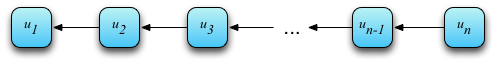
\includegraphics[scale=0.8]{4.Chapter2/Media/path_network.png} 
\caption{Example of a path network.}
\label{fig:path_network}
\end{figure}

In this graph, the size of the retweet group is, by definition, equal to the depth of penetration, as there is only one path (or retweet chain) available for propagation to occur along. As such, in each case, the retweet tree representing a resultant retweet group formed in this type of network will have the same structure as the graph itself, with a size dependent on the collective retweet decisions of the users.

Since each internal user has only one follower, the likelihood of each progressive user in the graph being able to view the Tweet in order to make the retweet decision reduces, and thus the retweet count is much more likely to tail off sooner than in graphs with more propagation avenues. This is also due to the fact that each retweet can only reach an audience of size 1 at each time step, and thus the `survival' of the Tweet cannot rely on a summation of many users' retweet decisions. The actual retweet \textit{decision} is not affected by a user's position in terms of `distance' from the source except through the effect of the regression features.

\begin{figure}[h]
\centering
\begin{tikzpicture}
 \begin{semilogyaxis}[
        xlabel=$|\rg{t}|$,
        ylabel=Frequency of occurrence,
        width=7cm,
        grid = major]
    \addplot[only marks,mark=+,blue] plot coordinates {
        (1,540)  (2,118)  (3,53) (4,27) (5,13) (6,5) (7,4) (8,2) (9,1) (10,0)
    };
\end{semilogyaxis}
\end{tikzpicture}
\caption{Frequency distribution of retweet group sizes in path network simulations}
\label{fig:linear}
\end{figure}

The likelihood of a particular user achieving the opportunity to receive the Tweet, in order to then retweet it, becomes the product of the probability function the further it travels through the graph, in which user $u_i$ requires each user from $u_1$ to $u_{i-1}$ to first receive it and then make a positive retweet decision. For example, if each user has probability $p$ of retweeting the Tweet, then each user's chance of receiving the Tweet is $\frac{1}{p^i}$, where $i$ is the position of the user in the graph. A user can only make a retweet decision on $t$ once it has been received.

The path network analyses involved 50 repeat simulations of the set of Tweets on a graph of size $n = 1000$. A timeline threshold ($H$) of 30 was used to represent the maximum time a Tweet is permitted on a user's timeline before it is no longer retweetable, for reasons discussed earlier. 

As might be expected, the frequency distribution of retweet group sizes in Figure \ref{fig:linear} shows a half-life type behaviour demonstrating the logarithmic pattern with many small retweet groups followed by a series of exponentially smaller groups. This user structure illustrates well how some users that might find the Tweet interesting, and who may then decide to retweet it, do not even get the chance to view it in order to \textit{make} that decision. Although this is accentuated in this structure, the same principle applies to any non-complete social graph, and demonstrates how the way in which users are connected can have a large impact on the overall retweetability of a particular Tweet.


\subsubsection{Random Network}

\begin{figure}[h]
\centering
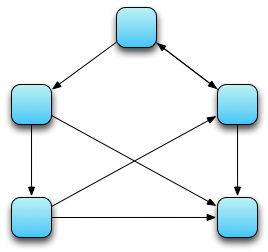
\includegraphics[scale=0.8]{4.Chapter2/Media/random_network.png} 
\caption{Example of a random network where $n = 5$ and $P_c = 0.5$.}
\label{fig:path_network}
\end{figure}

The random network was the next user structure to be analysed. Although it is certainly more similar to a real-life social graph than a path network, it is much more basic and uniform and does not consider user communities and clusters or different levels of influence in users in terms of differences in follower and friend counts.

A random social network is in this case based on the Erd\H{o}s-R\'{e}nyi model \cite{erdos60} and defined as a graph, $U = \left\{V,E\right\}$, where $n = |V(U)|$, consists of each user, $u \in V(U)$, having the connection probability $P_c$ of following each other $u_i \in V(U) \forall 0 \leq i \leq n$ and where $u_i \neq u$. Thus, as $P_c$ is increased, then so does the likelihood of $u$ following a $u_i$, causing the network to have a greater overall edge density. In general, therefore, the average number of followers and friends of a user is proportional to $P_c.n$. The only parameters needed for constructing such a graph are $n$ and $P_c$.

\begin{figure}[h]
\centering
\begin{tikzpicture}
 \begin{semilogyaxis}[
        xlabel=$|\rg{t}|$,
        ylabel=Frequency of occurrence,
        width=7cm,
        grid = major]
    \addplot[only marks,mark=+,blue]
       file {4.Chapter2/data/random.dat};    
\end{semilogyaxis}
\end{tikzpicture}
\caption{Frequency distribution of retweet group sizes in random network simulations}
\label{fig:random}
\end{figure}

As with the path network analysis, a graph size of $n = 1000$ was used under 50 simulations with the value of $H = 30$. The distribution in Figure \ref{fig:random} was generated using a value of $P_c = 0.01$, meaning that, on average, each user had 10 followers and 10 friends and was felt to be representative given the size of the entire graph.

The frequency distribution in Figure \ref{fig:random} demonstrates a very large proportion of mid-range values for $|\rg{t}|$, indicating that Tweets tend to have a consistent spread amongst the network, as might be expected. There are few smaller groups since there are no users that have disproportionately smaller spheres of influence, and each user has many incoming edges and a similar number of outgoing edges. This explains the smaller number of lower-range retweet group sizes observed in the distribution. However, as in any distribution so far examined, the number of larger retweet groups must eventually tail off due to the natural eventual reduction in positive retweet decisions being successively made as propagation chains increase in length.


\subsubsection{Scale-Free Network}
The final network structure examined in this section is the scale-free network. Also known as `small world', scale-free graphs are generally known to be representative of the general structure of `real-life' and online social networks \cite{mislove07} and, indeed, they are also used to describe the interconnections of real-world properties, such as friendship groups and food webs \cite{guido07} \cite{hein06}. Essentially, scale-free networks dictate that there are a small number of nodes with a high degree and many nodes with a low degree, and are usually generated through some form of preferential attachment algorithm. Thus, this type of network has support for the consideration of user communities and influential users in terms of those demonstrating a disproportionately large follower count. The other user structures studied do not have the scope for emulating this property of inconsistent interconnection between the user nodes.

Scale-free networks are constructed such that the distribution of the degree of the graph's nodes follow a power-law in that the distribution of the number of vertex edges across the graph is logarithmic. For these analyses, NetworkX\footnote{http://networkx.lanl.gov}, a Python graph and networking package, was used to generate directed scale-free graphs of users, based on a graph size, $n$, and various other arguments, including $\delta$-out, as the graph construction parameters. 

For the scale-free analysis, the same graph construction and simulation parameters were used as in the previous analyses. $\delta$-out represents the bias for a node's selection for out-degree from the other available nodes, and was set to a value of 0.7 to improve the clarity of the distribution result.

\begin{figure}[h]
\centering
\begin{tikzpicture}
 \begin{loglogaxis}[
        xlabel=$|\rg{t}|$,
        ylabel=Frequency of occurrence,
        grid = major,
         legend style={at={(0.5,-0.27)},anchor=north,legend cell align=left},
        legend entries={Twitter data, Generated scale-free data}]
    \addplot[only marks,mark=*,red]
       file {4.Chapter2/data/comparison-real.dat};
    \addplot[only marks,mark=*,blue]
       file {4.Chapter2/data/comparison-scale-free.dat};
\end{loglogaxis}
\end{tikzpicture}
\caption{Comparison of retweet group size distributions from scale-free graph simulations and data from Twitter's own social graph.}
\label{fig:real-scalefree}
\end{figure}

From simulations of the algorithm through these scale-free networks, a logarithmic trend is observed similar to that demonstrated from the `real' Twitter data analysed in the previous chapter and published in \cite{webberley11}, and the similarities in the distribution pattern is illustrated by Figure \ref{fig:real-scalefree}.


\subsection{General Comparison of Propagation Characteristics across Different Graph Structures}
In this section, three different network structures have been compared, and whilst the path network is very unrealistic as a representation of a social network, the differences in propagation behaviour presented by each do show how the interconnection of users on the graph can have a large effect on the spread of a Tweet. A small set of features to govern retweet features were used in order to accentuate the difference made by the user structures themseleves.

This has demonstrated that, in addition to the processes behind a user's individual retweet decision, the eventual spread of a Tweet also depends on how the original author's local network is arranged. Thus, the retweet decision of each involved user along with the available information pathways provided by the underlying social structure both contribute to the overall retweetability of a Tweet. 

If there are many edges in the network, such as in the case of the random network, then there are many more routes for peopagation to occur down to and from each user, due to the relatively large in- and out-degree of each user node on the graph. This increases the number of users who end up receiving the Tweet and then have the chance to make a retweet decision. This resulted in there being a larger distribution of larger retweet group sizes than smaller ones, before naturally diminishing again. 

\begin{figure}[h]
\centering
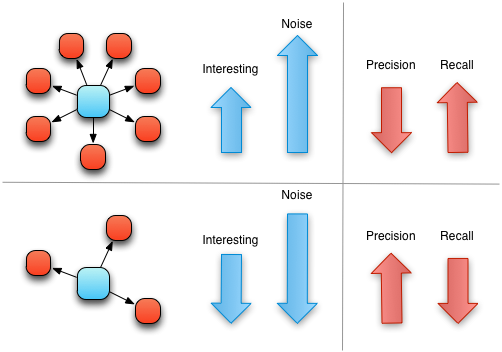
\includegraphics[scale=0.8]{4.Chapter2/Media/precision_recall.png} 
\caption{Comparing the effects of followship decisions on precision \& recall.}
\label{fig:precision_recall}
\end{figure}

Despite this high throughput of retweets, which provides a high level of information \textit{recall} for the users, the random graph structure is likely to demonstrate a low \textit{precision} in terms of the interestingness of the received Tweets. This is due to the large number of users having the opportunity to retweet the Tweet, increasing the chance that `noisy' information will be filtered through. As illustrated in Figure \ref{fig:precision_recall}, it is generally the case that if a person follows more users, they will receive exponentially more noise due to its prevalence over the interesting information (a decrease in precision), yet will likely receive more of the interesting information that is available (an increase in recall).

The path network demonstrated the opposite effect in that its nodes can only follow a maximum of one other node. This demonstrated very poor propagation, and required its simulation parameters to be altered to facilitate retweet behaviour more significantly than in the other graph structure analyses in order to produce any observable pattern. The results showed that propagation down a single allowed chain cannot be an effective way to spread Tweets, as it required each user in the chain to retweet it so that the successive users can have a chance to view it.

Similarly, in Twitter, users who follow very few others are likely to be more selective about who they follow. They will therefore achieve a greater precision in terms of the interestingness of information received, but the recall will be much smaller (Figure \ref{fig:precision_recall}). Generally, it is impossible to achieve a perfect precision and recall as it is likely that there will always be interesting information not being received, and any noise that is received at all will reduce the precision.

Whilst the scale-free network does not have the same general propagation throughput as the random network, it does demonstrate retweet patterns similar to those observed in data from Twitter's own social graph. This complements the findings of \cite{mislove07} and \cite{hein06} in terms of online social networks emulating real-life social networks having scale-free properties. This type of structure supports areas of the graph with denser communities, as is shown to exist by \cite{java07}, and have the potential for facilitating very large numbers of retweets if influential users are involved, but illustrate how Tweets `travelling' through less dense areas (and less-influential users) will not be as demonstrably popular.



\section{Using the Social Graph as a Method for Inferring Interestingness}
The graph analyses in the previous section have demonstrated a method for generating a $\rg{t}$ for a given Tweet, $t$. Since $\rc{t} = |\rg{t}| - 1$, then the same simulation algorithm can be used to estimate a retweet count for a given Tweet. The analyses conducted in the previous section relied on modelling the retweet \textit{decisions} made by the users, which individually account for that particular user's interest in that Tweet. Although it has been previously discussed that the overall retweet count cannot realistically be used alone for determining the level of interest in a Tweet, it is clear that interestingness of a Tweet is certainly based on a \textit{function} of the culmination of positive retweet decisions being made on the Tweet.

This notion is based on the idea that if a Tweet is more popular than the model predicts, then there is something about that Tweet that makes it more \textit{interesting} than similar Tweets that are less popular, such as a piece of breaking news or a link to a controversial article. For example, consider the case of two Tweets, written by the same author, and both containing the same instances of feature values in that they both contain a URL and mentions a user. If one of these Tweets achieves significantly more retweets than the other, then there must be some non-structural feature of the more popular Tweet that makes it stand out to the audience, and thus allows it to be perceived as more \textit{interesting}. This is because the features taken into account are static, and do not address any semantics of the actual content of the Tweet.

Similarly, if most Tweets of a user achieve between one and two retweets, then the expected retweet count for this user's future Tweets is likely to be similar. If, however, the author posts a Tweet which achieves an observed total of 10 retweets, then this is more popular than expected. If a Tweet achieves one or zero retweets, then this is as expected or less than expected, and is therefore not interesting.

\begin{myproposition}
\label{proposition:1}
The interestingness of a Tweet is a function of its expected and observed popularity. In particular, that a Tweet should be labelled as interesting if it is more popular than it was expected to be.
\end{myproposition}

This form of analysis is akin to anomaly detection and, in particular, the Helmholtz principle, which is defined by \cite{balinsky11} to be the deviation of interesting events from the randomness of the non-interesting events surrounding them. In the context of Proposition \ref{proposition:1}, exceptionally popular (or unpopular) Tweets can be represented by the interesting events, and the \textit{norm} of expected Tweet popularity is analogous to the randomness of non-interesting events.

Figure \ref{fig:helmholtz} helps demonstrate this behaviour in the context of Proposition \ref{proposition:1}, in which there is a `baseline' of expected Tweet popularity given by the properties of the Tweet and its environment. The exceptional, or anomalous Tweets, are the ones that are significantly different from the baseline; those that are much higher than this baseline are labelled as interesting since they are more popular than their features imply, and vice-versa.

\begin{figure}[h]
\centering
\begin{tikzpicture}
\begin{axis}[
        ylabel=Tweet popularity,
		xlabel=Feature amalgamation,
		ymax=200,
		xmax=20,
		xmin=0,
        yticklabels={,,},
        xticklabels={,,}
        ]
    \addplot[only marks,mark=+,blue] coordinates{
        (0,3)(1,6)(2,8)(3,17)(4,21)(5,27)(6,29)(7,35)(8,39)(9,48)(10,52)(11,53)(12,59)(13,61)(14,67)(15,71)(16,73)(17,81)(18,85)(19,92)(20,100)
    };
    \addplot[only marks,mark=+,blue] coordinates{
        (3,37)(5,59)(10,11)(14,130)(18,23)
    };  
\end{axis}
\end{tikzpicture}
\caption{Conceptual example illustration of Tweet popularity as a function of their properties}
\label{fig:helmholtz}
\end{figure}

As such, a method is proposed based on the following two criteria;
\begin{itemize}
    \item $\rc{t} > \ec{t} \Longrightarrow t$ is interesting
    \item $\rc{t} \leq \ec{t} \Longrightarrow t$ is non-interesting
\end{itemize}
where $\ec{t}$ is the expected retweet count of $t$.

Although it was found in the previous chapter and in other relevant literature that pseudo-generated scale-free networks can be representative of Twitter's own social structure, a user's actual own local social network would more accurately portray the links between the users surrounding the original author of a Tweet. By constructing a network based on a user's own local network, then the method would effectively be simulating the Tweets' propagation through the edges representing the followships of the real and appropriate users in Twitter's social graph.

Thus, in the simulations, the user in question is $\aut{t}{O}$, $t$ is the Tweet to be simulated and initially $S = \fos{\aut{t}{O}}$. At each timestep, each user in $S$ would have the opportunity to retweet $t$, and therefore, by running the simulation multiple times, an estimation of $\ec{t}$ can be obtained.\\
In particular, the method follows these steps;
\begin{enumerate}
    \item Select a user, $u$, from Twitter to be $\aut{t}{O}$
    \item Collect $u$'s local follower network 
    \item Collect a set of $u$'s recent Tweets
    \item Construct a network based on the users and edges of the collected network
    \item Simulate the collected Tweets through the constructed network using the simulation algorithm.
\end{enumerate}

This procedure would provide an estimated retweet group size for each Tweet, which could then be compared to the actual observed retweet count of the Tweet on Twitter to help towards deducing the interestingness.


\subsection{Data Collection}
Ideally, the entire social graph would be used, but due to the scaling properties encountered in a breadth-first traversal of Twitter's social graph, it became infeasible to collect a user's local network containing users more than two edge `hops' away from the source user under the rate limitations of Twitter's REST API. As previously described, v1 allowed 350 calls to the API each hour for each authenticated Twitter account. One call, for example, was required to obtain a list of up to 5,000 user IDs representing the followers of a particular user - the users one hop from the source user. An additional call would then be required to collect each of these user's own followers in order to provide the 2-hop representation of the local network from the source user.

For a user with a follower count of 700, a total of 701 API calls would be required to collect the user's local network within two hops - the one to retrieve the source user's immediate followers, and then one further call for each of the 700 followers. This would take over two hours of collection, and to collect the third hop would require another exponential number of API calls. If each of the 700 followers of the source user has, on average, 200 followers, then this would require  a further $700 \times 200 = 140,000$ API calls, which, in total, equates to over 402 hours of data collection time. Although some follower overlap is likely to be present among the users two hops away, when one considers that this is simply the time taken to collect the local network for \textit{one} user, then it becomes clear that this must still be an impractical approach.

Observation \ref{observation:path-length} states that the vast majority of retweets do actually occur \textit{within} two hops of the source user, in that the most significant number of retweet groups analysed had a maximum path-length of less than three. In addition, as mentioned, online social networks are `closer' than real-life social networks, and was found to have a value of around four degrees of separation in Facebook. These points help to justify the decision made to classify a user's local network as those users and edges existing within two hops from the source user.

In June 2012, the Twitter REST API was used in order to conduct a random walk through Twitter's social graph. Starting by selecting an initial user, an edge expressing the followship of a random follower was chosen in order to select the next user. This continued for each of the selected users in turn and, for each user selected, the most recent 300 Tweets and surrounding information was collected along with that user's local follower network within two hops. The friend network (i.e. the outward edges from each user) was ignored, as only the directional outward flow of information from the source user was useful in this experiment. If, at any stage, the currently selected user did not have any followers, the collection algorithm backtraced to the previous user and another follower was selected instead. The crawler continued until the rate limit for the current request window was met, at which time the current data state was stored, and then waited until the rate-limit was reset before continuing.

The data collection resulted in a set of 33 Twitter users, each with a full 2-hop local network collected and a set of up to 300 Tweets. In total, around 10,000 Tweets were stored as a result of the crawl to be used in the simulations. It was decided that the previously trained regression model would be re-used as part of the retweet decision engine in this experiment also, and so no further training data was required to be collected. From the Tweets collected, the \textsc{url} and \textsc{mentioned} features could easily be indentified, and the two user features could be extracted under the same process as the one used in the network simulations in the previous section.

For each Tweet collected, a simulation could now be run in order to provide an expected retweet count for that particular Tweet. By comparing this value to the actual retweet count expressed by the Tweet, which is returned as part of the standard Twitter API call, an indication of whether or not the Tweet is interesting could be obtained.



\subsection{Validating the Accuracy of Inference Results}
In order to test the validity of the results, it was necessary to use human asessment on each of the evaluated Tweets to check for agreement between the interestingness inferences made by the algorithm and by humans. Although interestingness is a subjective notion, the validations were carried out in such a way to emphasise a \textit{global} level of interest in terms of the general separation between noisy and un-noisy Tweets.


\subsubsection{Crowdsourcing Validations}
Crowdsourcing is a technique that has grown in popularity over many domains in recent years, including  media, reviews services, sensor networks, and others. Essentially, crowdsourcing involves the use of many people (or, in some cases, devices) providing input or results on a given task. Services such as Google Maps\footnote{http://maps.google.com}, TripAdvisor\footnote{http://tripadvisor.co.uk}, and Stack Overflow\footnote{http://stackoverflow.com} respectively use crowdsourcing for obtaining information (such as photos) on geographic locations, service reviews, and programming assistance. Its use means that the crowdsourcers can easily receive lots of input with very little additional work, since the load is spread amongst many people.

Crowdsourcing has also proved to be a useful asset in research as it facilitates the harvesting of many inputs, from diverse opinions and views, much more quickly than without it, and it is a useful tool for validating data. Many crowdsourcing services are active on the Internet to cater for different use-cases.

Amazon's Mechanical Turk\footnote{http://mturk.com} allows crowdsourcers to create small jobs (known as `microtasks') to be completed by crowdsourcees, known as Mechanical Turk Workers (MTWs), who have an account on the website. The crowdsourcer describes the particular microtask in terms of what is expected of the MTWs and also determines the amount paid for the task. A single microtask completed by a particular MTW is known as a `judgment', and MTWs are paid for each judgment he/she completes. The crowdsourcer can define certain criteria on the microtasks, such as allowing each MTW to only complete one microtask.

Due, at this time, to Mechanical Turk's availability to only US credit card holders, a third-party service, Crowdflower\footnote{http://crowdflower.com}, was used instead to submit the microtasks to Amazon's system in order to be completed by the workers. 


\subsubsection{Aims of the Validations}
The purpose of the use of crowdsourcing was for evaluating the effectiveness of the interestingness inferences made through the aforementioned comparison between an expected and observed popularity of a given Tweet. In particular, of concern was the correlation between those Tweets that the algorithm denoted as interesting and the Tweets that humans found interesting.

Since the accuracy of the various components of the technique could not be known until they were properly validated, it was decided that the crowdsourcing would initially be run as a pilot test in order to identify the presence of any correlations. If this was sufficiently successful, then a further and more rigorous test would take place, involving more workers.


\subsubsection{Constructing the Questions}
The microtasks presented to the MTWs each consisted of a question containing five Tweets that were selected at random from the experimental set. Each question asked the MTWs to select which one of the five Tweets was the most interesting and which one was the least interesting. The validations were set up so that each of the questions was assessed by at least three different MTWs.

\begin{figure}[h]
\centering

\includegraphics[scale=0.8]{4.Chapter2/Media/mtk_question.png} 
\caption{Example question for the MTWs: "Select the most interesting Tweet and the least interesting Tweet from the five shown"}
\label{fig:mtk_question}
\end{figure}

Figure \ref{fig:mtk_question} shows an example of a question asked of the workers. It demonstrates also how the MTWs were not provided with any additional context, such as the author's username or the post date and time, for any of the Tweets to be evaluated.

Although Tweet selection was random, those whose content starts with a user's ``@'' username (i.e. `@-replies') were excluded, since these Tweets typically form part of a conversation between a small number of users and are unlikely to convey any interest to those not directly involved. The final validation set consisted of a total of around 4,500 Tweets to be assessed in the questions, and MTWs were encouraged to follow links to any websites or media included in the Tweets' contents as part of their evaluations.


\subsubsection{Inference Performance Validation Results}
The Mechanical Turk validation take place between the 7th and 11th December 2012. Table \ref{table:mtk_data_1} provides further information about the validation tests. An assessment is defined as a MTW answering a particular question with his/her opinion on the most interesting and least interesting Tweet. Since there were 856 questions, there were 2568 assessments in total.

\begin{table}[h]\footnotesize
\begin{center}
\begin{tabular}{ l || c }
	 Total assessments by MTWs & 2568\\
	 Number of distinct questions & 856\\
	 Number of unique MTWs & 177\\
	 \hline
	 Num. questions with $\geq \frac{2}{3}$ agreement on most interesting & 510\\
	 Num. questions with $\geq \frac{2}{3}$ agreement on least interesting & 493\\
	 \hline
	 Amount paid to MTWs per assessment & \$0.03\\
     \hline
\end{tabular}
\end{center}
\caption{Information on the Mechanical Turk validation results.}
\label{table:mtk_data_1}
\end{table}

A confident answer is defined as the case in which at least two of the three MTWs answering a particular question agree on the most interesting and least interesting of the Tweets. It is assumed that if at least two people agree on a piece of content being interesting, then this provides further strength to the individual assessments, and any questions that were not confident were excluded from the following validation analysis.

Through the retweet simulations and algorithm for each Tweet, an 86\% accuracy was achieved in terms of correctly predicting the actual retweet count - the cases where the expected retweet count is equal to the observed retweet count. In around 30\% of cases, a Tweet that was determined to be interesting through the methodologies described in this chapter was also verified as interesting by the agreeing MTWs.

This is a relatively low accuracy, and while it does mean that the method was able to correctly identify an interesting Tweet from a set of five in 30\% of cases and the random performance of selecting an interesting Tweet could not reach this accuracy, it is not a strong enough result to describe the method as being suitable in the general inference of interesting Tweets. 

As such, further investigation would be required to address the method with the aim of improving this performance.


\subsection{Improving The Interestingness Inference Performance}
The deduction of the interestingness of a Tweet through the comparison of the expected and observed popularity of that Tweet is considered a viable way of addressing the problem for reasons discussed earlier. However, a more convenient and accurate method is clearly required for acquiring the \textit{expected} retweet value.

The issue with the current method is two-fold; as mentioned, lots of data is required in order to reconstruct the Tweets' authors' local networks in which to simulate the Tweets, which leads to the second problem of only being able to simulate Tweets from authors in sparser local networks. Under the current scheme, only users with a small enough local network (i.e. users that have lower folower counts) can realistically be evaluated, due to the collection criteria discussed previously, meaning that the methodology cannot be used in the general case. Although a high accuracy was achieved in predicting the \textit{correct} retweet counts for the Tweets assessed in this section, most of these Tweets only actually had an observed retweet count of 0 or 1. This is the by-product of the previous issue in that only users with fewer followers could have their Tweets simulated, and these users will therefore typically receive few retweets per Tweet. Ideally, the methodology should have the capabilities to be applied to any type of user and any Tweet on Twitter.

Additionally, this method alone does not make efforts towards evaluating the \textit{level} of Tweet interestingness. Instead of the binary interesting / non-interesting decision, it would be more useful to award each Tweet a score denoting the estimated interestingness of the Tweet. The further importance and usefulness of this is explained in further detail in the following chapter.


\section{Chapter Summary}
In this chapter, an analysis of propagation through differing structures of user connections on social graphs has been conducted. From this, a potential methodology for inferring interestingness of Tweets has emerged, which, despite being negatively impacted by various factors in its current form, shows promise as a suitable technique towards assisting in this task.


\subsection{Network Structure Analysis}
A logistic regression model was built as part of a simulation algorithm in order to anaylse the propagation characteristics of three different network structures; a path network, a random network, and a scale-free network. 

Although the actual retweet counts of simulated Tweets in each network structure are not comparable due to the parameter alterations that were required in order to amplify visible results, the actual \textit{pattern} of propation in terms of the distribution of retweet group sizes was found to be different in each structure and for differing reasons. In addition, the scale-free network was found to express a similar pattern to that observed from the data on retweet group sizes discussed in the previous chapter.


\subsection{Interestingness Inference Methodology}
The model and techniques behind the network structure analyses were then applied to the goal of detecting the interestingness of Tweets based on the comparison of the expected retweet value, generated through the same algorithm used to simulate Tweets in the network analyses, and the actual observed retweet count of the Tweet.

Validating the methodology showed that the technique is not particularly useful in determining interesting information, and its other drawbacks, such as its application only realistically being available to Tweets from non-influential users, mean that the technique cannot be used in the general case. Further to this, the data collection required is not suitable for quick evaluations and may not remain accurate over time even after collection due to the continuous changing nature of the edges in online social networks as users create and destroy followships. This is particularly impactful in this case as there are many users involved even in a user's 2-hop local network.

In the next chapter, the methodology for generating expected retweet counts is adapted with the aim of improving its validation performance, the ease of preparation through data collection, and of addressing the methodologies current restrictions on the types of users it is suitable for. It is known from work in this chapter that the network structure plays an important role in information propagation, so this and more environmental features are taken on as part of the improvements. This research then leads to the production of a technique for measuring \textit{how} interesting a particular Tweet is, including the way in which this can be calculated and the different validations performed against it to assess its performance.

\chapter{Development of the Interestingness Inference Methodology}

Research in the previous chapter focussed on researching the effect of the social graph on retweet propagation characteristics. From this, a methodology, displaying a range of various shortcomings, emerged based on Proposition \ref{proposition:1} and the models and simulations utilised in the graph analyses. In this chapter, the methodology is modified with the aim of improving its performance and increasing the range of use-cases it is appropriate for. Since the social structure was found to play an important role in propagation, many network and user features are taken into account throughout the improvements and investigation.

In addition, modifications are made in order to provide an indication of \textit{how} interesting a piece of information is estimated to be, and more about this particular component is discussed in later sections.

The proposed methodologies also relate to the differences highlighted between a Tweet's raw popularity, as indicated by its retweet count, and how interesting the Tweet actually is to those who read it. It has been shown that making retweet predictions against models trained with a large number of features can be accurate \cite{zhu11}, but in this work the focus is more on the Tweet's content and properties beyond the static features. That is, that when comparing Tweet popularity, then there may be some content, either within the Tweet itself or perhaps in a resource indicated by a URL contained in the Tweet, that makes the Tweet stand out more to its recipients and to cause the aforementioned notion of \textit{affective stimulation} \cite{xu07} to its viewers.

Of course, this brings about the notion of information \textit{relevance}, and the fact that the same Tweet could be very boring or irrelevant to one user, and very interesting to another. In this work focus is applied to \textit{global} (or `average') interest, where interestingness inferences are made for the general case. It is considered that Tweets that are retweeted more than expected within their authors' local networks, relative to the usual retweet count of the authors' other Tweets, are also likely to be of interest to a wider audience, especially since they are now more likely to penetrate through the social graph enough to be received by users in different communities.
 
As such, the focus of the work in this chapter is that of adapting the inference methodology in order to develop a technique for accurately \textit{quantifying} the interestingness of Tweets. This is concerning universal relevance in terms of highlighting interesting Tweets from the noise. In particular, there are two main improvements over the previous methodology to be made;
\begin{itemize}
    \item Improve the method for generating the \textit{expected} retweet count of a Tweet (in terms of accuracy and range of application);
    \item Expand the binary retweet interesting inference into a more useful scale in order to support the \textit{ranking} of information by interest.
\end{itemize}


\section{User Influence}
As has previously been posited, of importance to this work is the difference between the retweet count of a Tweet and the interestingness of the Tweet. An example in the Background chapter was provided, which was related to the case of Justin Bieber. His account, \texttt{@justinbieber}, is one of the most `influential' on Twitter, with nearly 50 million followers at the time of writing. His Tweets receive an average of around 50-120 thousand retweets per Tweet, and they rarely receive fewer than 40,000 retweets. Since an average Twitter user would generally attract a maximum of a few hundred followers, and would normally receive very few, if any, retweets per Tweet. A particularly interesting Tweet from such a user may be retweeted, for example, between 5-20 times. It is therefore apparent that, in the general case, an uninteresting Tweet from an influential user may receive 50,000 retweets, and an exceptionally interesting Tweet from a less-influential user may be retweeted 30 times. It is therefore clear that user influence dictates that this value cannot alone be indicative of Tweet interest.

However, since interestingness \textit{does} have an effect on an a user's individual retweet decision on a particular Tweet, this absolute retweet count can be used as part of the method for generating an interestingness \textit{score} for that Tweet.


\section{Interestingness Quantification through Tweet Scoring}
To address the notion of interestingness quantification, a scoring scheme is hereby introduced, allowing certain interesting Tweets to be ranked as `more interesting' than other interesting Tweets. This, in itself, is an improvement over the previous method, which allowed only for Tweets to be labelled as `interesting' or `non-interesting'.

As an enhancement to Proposition \ref{proposition:1}'s \textit{comparison} between the observed and expected retweet counts, the new scoring technique is based now on the \textit{distance} between the two counts. The general idea and potential use-case for this is that if a score is known for a set of Tweets, then these can be used as a basis for ordering information as part of information retrieval or an information delivery system, where Tweets can be displayed to users in a more useful way than simply chronologically, and where interesting Tweets could be brought forward to users who don't follow the source user or a retweeter, and thus deliver information to an interested user, yet without him or her having to know about it first.

\begin{myproposition}
\label{proposition:2}
If the positive difference between a Tweet's observed and predicted popularity is proportionately greater than those attributes in a different Tweet, then the first Tweet is proportionately \textit{more} interesting than the second.
\end{myproposition}

Essentially, Proposition \ref{proposition:2} stems from the following scenario. Consider two Tweets, $A$ and $B$, which have the following properties;
\begin{itemize}
    \item $\ec{A} = 3000$ and $\rc{A} = 3010$
    \item $\ec{B} = 5$ and $\rc{B} = 15$
\end{itemize}
Where $\ec{A}$ and $\ec{B}$ represent the expected retweet count of $A$ and $B$ respectively.

In this case, both Tweets would have been flagged as `interesting' under Proposition \ref{proposition:1} (although, in reality, the derived method would not be able to model users who are typically expected to achieve 3,000 retweets). However, it is clear that, despite the \textit{difference} between the counts being equal, Tweet $B$'s observed retweet count is actually much more significantly proportionately greater than what was expected, and is therefore likely to be more significantly interesting.

Since the proportionate difference is the key to this, the interestingness score, $\score{t}$, for Tweet $t$ is simply given by;
\[
\begin{array}{cc}
 \score{t} = \frac{\rc{t}}{\ec{t}}
\end{array}
\]

This provides a positive score where;

\[
\score{t}
	\begin{cases}
		> 1		&	\text{indicates } t	\text{ is interesting} \\
		\leq 1	&	\text{indicates } t	\text{ is non-interesting}
  \end{cases}
\]
and where $\score{A} > \score{B}$ implies that $A$ is more interesting than $B$.

Since this methodology relies on data collection from Twitter in order to obtain the observed retweet counts, it involves extracting a snapshot of the state of the evaluated Tweets at one stage during their lifetime. Since Tweets are not removed over time, unless they are deleted by their author, they can be discovered and retweeted at any time after their composition and posting.

The work in this chapter assumes that the most significant portion of retweet activity for a specific Tweet has already occurred by the time the information on the Tweet has been collected. Indeed, the authors of \cite{kwak10} carried out investigative analyses into various temporal retweet behaviours, and discovered that, on average, a Tweet receives around 75\% of its retweets within the first day of being posted. 50\% of the retweets of a Tweet even take place within the first \textit{hour} of the Tweet being posted. Due to this, and to ensure that the retweet count collected is mostly representative of the Tweet's exraploated `final' retweet count, only Tweets that had been posted at least one day ago were considered for experimentation.


\section{Further Adaptations of the Inference Methodology}
In the previous chapter, it was noted how it was necessary to improve the method used for producing a Tweet, $t$'s, expected retweet count, $\ec{t}$. Limitations with the previous method dictated that it could only work under certain restrictions. In particular, that the user must have a small enough local network (in practice, a follower count of more than 500 or so made the method very unsuitable), and that, due to this, Tweets only attracting very few retweets could effectively be simulated. In addition, the interestingness inferences made were not significantly accurate, although this is likely due to a combination of the above issue in providing much less room for error and the fact that the interestingness decision was only binary.

A new method is hereby proposed, derived from Proposition \ref{proposition:2}, for carrying out the prediction for the value of $\ec{t}$. This method is immediately more superior to the previous, as only a very small amount of data is required to be collected from Twitter. This means that inferences on Tweet interestingness could be made on demand\footnote{Not `live' as it relies on time for retweets to have occurred.}.

Essentially, the method involves generating a classifier model capable of producing a base-line expected retweet count for a given Tweet and its relationship with its author. In this case, the classifier would be trained with the Tweet's actual retweet \textit{count} instead of the binary retweet decision used previously, and it would not require the simulations of the user's local network. Many more features regarding the Tweet, and its conetent, and its author are used to represent the particular user-Tweet information required for generating the predictions.

Since the graph structure clearly has an impact on message propagation, then it was felt that a significant consideration should be made towards including features relating to the interconnection of users, such as follower counts, Tweet rate, and information on a sample of friends and followers. More detail on the features used is provided in later sections.

In general, the newly proposed methodology follows these basic steps:
\begin{enumerate}
    \item Collect sufficent data from Twitter to train a classifier with an appropriate set of features. The trained model is known as the `global' model;
    \item Obtain a Tweet, $t$, and extract its own features as well as information about its author and its author's local graph properties;
    \item Classify the Tweet's features against the trained classifier to produce a retweet count prediction, $\ec{t}$ for this feature instance;
    \item Calculate \score{t} through using this $\ec{t}$ value and the known $\rc{t}$.
\end{enumerate}

In addition to this `global' model, a `user' model was proposed to be built for each user being evaluated. This user model would be much smaller, as it would only contain information on a history of that user's Tweets, but would be capable of providing a second value for $\ec{t}$ when testing Tweets against it. With two such values generated through the comparisons of Tweets to both the global and user models, two scores could be generated as a function of the static value of $\rc{t}$.

As such, the two scoring mechanisms work as follows;
\[
    \gscore{t} = \frac{\rc{t}}{\ecg{t}}
\]
\[
    \uscore{t} = \frac{\rc{t}}{\ecu{t}}
\]
where $\gscore{t}$ is the score generated from comparisons to the \textit{global} model and where $\uscore{t}$ is the score derived from the model representing the historical Tweets of $\aut{t}{O}$.

\section{Retweet Volumes as Nominal Attributes}
Most machine learning classifiers are not useful in accurately predicting the outcome of a feature of a large-ranging and continuous data type. Instead, the performance can be greatly improved when making predictions from a limited range of discrete ranges, or `nominal' data.

Thus, in order to help improve the accuracy of $\ec{t}$ predictions, it was decided to convert the retweet count feature into a nominal data type for the purposes of training the model and making classifications. By `binning' the retweet counts into categories representing interval ranges, there would be fewer outcome possibilities, and thus the \textit{confidence} of classifcation could be greater.

The values for $\score{t}$ would then be determined through the ratio of $\rc{t}$ to the upper-bound of the nominal range category containing $\ec{t}$.


\subsection{Binning the Retweet Counts}
Since a trained classifier is only generally able to make predictions on features and values it has prior knowledge of, the bin ranges for each category must be equal in both the training feature data and the testing feature data. If the available nominal values for an instance feature representing a Tweet has a different set of category ranges to that in the trained classifier model, then it is likely that a prediction cannot be generated for this instance. It was therefore necessary to consider this when determining a method for binning the retweet counts.

There are various ways in which the counts could be binned, and all begin with a decision on the number of bins to use. The varying performance of this factor is considered later.

Initially, retweets were binned in a \textit{linear} fashion. That is, that the full range of retweet counts in the training set was calculated and then split into bins such that each category had as equal a range as possible. If there were no cases where $\rc{t} = 0$, then a category representing $[0,l)$, where $l$ is the minimum value for the lowest range, was pre-pended to the set of available nominal categories. Similarly, in all cases, the interval $[m+1,\infty)$ was appended to the set of categories, where $m$ is the maximum value in the highest range. This dictates that no Tweet in the training set can have a value for $\rc{t}$ in this category, and thus this allows any Tweet to potentially have $\score{t} > 1$ when \textit{testing} against the model. For example, if a training set of Tweets had a total range of values for $\rc{t}$ being between 1 and 20 was binned into four ranges, then the following interval categories would be applicable:
\[
    [0,1) [1,6) [6,11) [11,16) [16,21) [21,\infty)
\]

Since the distribution of retweet counts (expressed through retweet group sizes) is known \cite{webberley11}, then it is clear that this binning methodology would produce bins containing a very non-uniform distribution of Tweets, where the lower bin ranges would contain many Tweets and the cardinality of each category would decrease exponentially as the cateogories become higher. This means that there would be fewer feature instances representing Tweets with larger retweet counts.

 Indeed, when training classifiers and running cross-validations on these, this binning scheme demonstrated a high accuracy of predictions on Tweets with lower values for $\rc{t}$ and a low accuracy for Tweets with higher counts. It would be more appropriate, and better address the desire for more universal use-cases expressed earlier in this and the previous chapter, if the accuracy of predictions could be more uniform across the bin ranges.

Various other methodologies were implemented, which eventually evolved into a histogram-based responsive binning algorithm. Essentially, this algorithm is based around the initial calculation for the projected size of each bin, which is obtained from the total number of Tweets to be categorised and the target number of bins. Each bin was then filled according to the interval range specifying the bounds of that bin, and in such a way as to ensure that each retweet count frequency would only be present in one bin. For example, all of the retweets achieving one retweet would be placed in the single bin encompassing this value.

As such, after the intervals representing the bin bounds have been produced, then these represent the nominal categories for the retweet count feature in each instance for training and testing against the classifier.



\newfloat{algorithm}{H}{lop}
\begin{algorithm}
\caption{Algorithm for producing intervals for bin categories for $\rc{t}$ values.}
\begin{algorithmic}[1]
\Procedure{generate\_intervals}{set of Tweets $T$, number of bins $B$}
    \State $C\gets$ empty list \Comment{To hold ordered retweet counts}
    \State $I\gets$ empty list \Comment{To hold bin range intervals}
    \ForAll{$t \in T$}
        \State Add $\rc{t}$ to $C$
    \EndFor
    \State Sort $C$ into ascending order 
    \State $M\gets\max(C)$ \Comment{Highest instance of $\rc{t}$}
    \State $T\textrm{Sum}\gets\frac{|C|}{B}$ \Comment{Number of Tweets in each bin}
    \State $H\gets$ empty dictionary \Comment{Histogram of retweet count distribution}
    \Statex
    \ForAll{$c \in C$}
        \If{$c \in H$}
            \State Increment $H_c$
        \Else
            \State $H_c\gets0$
        \EndIf
    \EndFor
    \ForAll{$i$ in range $M+1$}
        \If{$i \in H$}
            \State $s = s + H_i$
        \EndIf
        \If{$s \geq T\textrm{Sum}$}
            \State Add $i$ to $I$
        \EndIf
    \EndFor
    \State Return $I$
\EndProcedure
\end{algorithmic}
\label{algo2}
\end{algorithm}
 
This new responsive method readily supports more uniform bin sizes, and copes with this by exhibiting exponentially larger bin \textit{ranges}. As such, the distribution of bin sizes is generally described by a distribution simular to that shown in Figure \ref{fig:bin-hist}. As with the linear method, the interval $[0,l)$ is pre-pended, where necessary, and $[m+1,\infty)$ is always appended in addition to the intervals produced by the algorithm.

\begin{figure}[h]
\centering
\begin{tikzpicture}
\begin{semilogyaxis}[
    symbolic x coords={[0-1), [1-2), [2-3), [3-4), [4-5), [5-100)},
        ylabel=Cardinality of bin,
		xlabel=Bins,
        ybar,
        bar width=7pt,
        yticklabels={,,},
        xticklabels={,,}
        ]
   \addplot[plot 0,bar group size={0}{1}]
        coordinates {([0-1),100) ([1-2),50)  ([2-3),50) ([3-4), 50) ([4-5), 50) ([5-100), 25)};
        
\end{semilogyaxis}
\end{tikzpicture}
\caption{Visual example distribution of retweet count bin cardinalities under the responsive binning algorithm}
\label{fig:bin-hist}
\end{figure}

This method is responsive in that the bin ranges adapt to the variety and number of retweet counts available, and it always attempts to produce a similar number of bins to the target count. However, due to the disproportinately large number of small retweet groups, the bin sizes cannot be entirely uniform and this means that the number of bins returned will generally be smaller than the target number.

This also stems from the fact that a single retweet count cannot exist in more than one bin concurrently; for example, if the interval $[0,2)$ existed in a scenario, and the number of Tweets with retweet count equal to 0 or 1 is greater than the value for $T\textrm{Sum}$, which is often the case, then this will result in a larger bin. Without this particular feature, training Tweets with equal observed retweet count may be categorised into multiple bins, causing the eventual prediction accuracy to be reduced. 

Due to this dynamicity, the bin ranges and cardinalities produced by the algorithm vary across different datasets. As a result, the nominal bin categories generated for producing the value for $\uscore{t}$ from the user model trained from the complete set of collected Tweets posted by $\aut{t}{O}$ would be different from those categories generated for a different user. The intervals in each bin category are therefore reflective of the various numbers of retweets that each author's Tweets are likely to receive. 


\section{`Twitter is a Memepool'}
In 1976, Richard Dawkins coined the term `meme' to be defined as a ``unit of cultural transmission'' \cite{dawkins76}. The general idea behind memetics is as an analogy to biological genetics except, unlike genes, memes are entirely non-physical and represent a cultural idea or aspect or another human-based behaviour. The rise of social networks on the Internet has allowed the spread of memes to grow to the extent that they are sometimes now even represented by `physical' constructs, such as images.

In genetics, a gene is a physical entity containing information and instructions. It is a unit of genetic inheritance, in that they are passed from parent to offspring through the act of reproduction, and the result of an organism having a gene is that the organism will express the features represented by that particular gene. These genes contain instructions that make up the features of an individual, such as physical characteristics like eye colour and height, and non-physical characteristics, including various aspects of personality.

Organisms exist in an evironment that also has features, such as humidity, altitude, temperature, relationships to other organisms, and so on. If the genes of an organism are such that they cause the individual to be well-suited to its environment, then that organism has a better chance of survival and, therefore, a better chance of achieving reproduction.

Memes are similar in that they are effectively made up of a set of features, or a `memome', such as the wordings of a particular phrase, or their relevance to other cultural aspects. These enable the meme to be less or more likely to be replicated in different environments, which is made up of the humans exposed to it and the interactions between them. For example, an Internet meme relating to the Star Wars movies would likely have a greater chance of being reproduced, through discussion and reposting, in an environment comprising a set of science-fiction fans than when amongst more mixed-interest groups.

The meme is also a useful analogy in this thesis when describing the way in which Tweets undergo replication within Twitter. Like a meme, a Tweet has a specific set of features, such as the text it contains, the inclusion of any mentions or a URL, and so on, and it exists within an environment consisting of a set of interconnected users on the Twitter social graph. A particular Tweet would generally have a greater chance of `surviving' and being replicated, through the act of retweeting, amongst a certain subset of users intereconnected in a particular way than in other environments.

As such, the Tweet features are analogous to the \textit{genes} of a genome, and the arrangement and type of users on the social graph that receive the Tweet and have an opportunity to assist in its propagation comprise the Tweet's \textit{environment}. Since the environment has previously been found to have a large effect on propagation, then these features are useful aspects to include as part of the improved methodology covered in this chapter.


\section{Generating Values for $\ec{t}$}
In order to generate the estimated retweet counts, a trained machine learning classifier is needed to make predictions on a set of feature instances. This section covers an overview of the classifier used for this purpose, including a justification in terms of an analysis of its performance.


\subsection{The Classifier}
An overview of machine learning classifiers and their processes was provided in the previous chapter. In that case, a logistic regression was used to generate a prediction on a binary retweet decision based on a small number of features. If the retweet count for the Tweet being trained or tested was greater than zero, then the retweet decision would be positive (\textsc{True}). Otherwise, the decision was negative (\textsc{False}).

Presently, the new methodology involves the prediction of a retweet count category from a set of nominal values of cardinality greater than one. As mentioned, the instances of a particular Tweet and its evironment are categorised based on the value of the retweet count of the Tweet. Although this means that a degree of accuracy is sacrificed when training the classifier, it does mean that there are fewer categories for predictions on test Tweet feature instances, providing a higher confidence for each prediction made.

The Bayesian network machine learning classifier was elected for use for the purposes required in this chapter. Use of this classifier in the social media domain is more rare than other classifiers, such as those involving a regression or a decision tree, but was selected for the various reasons highlighted later in this section.

The Bayesian network is an unsupervised classifier since its learning algorithms do not simply determine the class of the outcome, the retweet count, from the attribute features alone \cite{friedman97}. Instead, a probabilistic graph is constructed based on the dependencies between the variables. The variable attributes form the nodes of the graph and edges between the nodes denote the dependencies (or lack thereof) between them.

Thus, in the case of this research, the various Tweet and envirnomental features, including the nominal retweet count, form the nodes in the Bayesian Network. When forming the network through training, the dependencies and their probabilistic weightings are adjusted so that an expected value for the retweet count can then be `predicted' from the values of all the other variable attributes.


\subsection{Classification Performance}
When selecting classifiers, the Weka\footnote{http://www.cs.waikato.ac.nz/ml/weka} machine learning and data mining toolkit was used to evaluate the relative performance of various types of appropriate classifiers for the task. The classifiers were selected to cover a sample of the range of available classifier categories. Whilst some types may work inefficiently in this scenario, it is likely that they are more efficient when employed in different use-cases.

Although the accuracy of prediction was important, it would also be useful for the classifier to be \textit{efficient} in training its model and when testing future instances against it. This is so that this method could be used to produce interestingness inferences with a more on-demand policy and to further improve on the methodologies used in the previous chapter.

\begin{table}[h]\footnotesize
\begin{center}
\begin{tabular}{ l | c | c | c }
	Classifier	& Precision & Accuracy (recall) &  training time (secs.) \\
	\hline
	\hline 
	Simple logistic & 52\% &  56\% & 528\\
    Logistic        & 62\% &  56\% & 18\\
    SMO             & 51\% &  55\% & 1384\\
    Na\"{i}ve Bayesian & 50\% & 44\% & 0.13\\
    Bayesian network & 62\%&  64\% & 0.54\\
    \hline  
\end{tabular}
\end{center}
\caption{The training performance of different machine learning classifiers.}
\label{table:classifierperformance}
\end{table}

The Bayesian network was found to be accurate and time efficient when evaluating the performance of the set of evaluated classifiers. A dataset, obtained as part of the general data collection (please see the relevant section below) and which contains a set of over 57,000 Tweets, was identically used in each of the analyses. For each Tweet instance the same retweet count binning scheme was used, and each classifier performed the same number of cross-validations against the same dataset in order to obtain the precision and recall values.

Although the dataset used in this analysis is not the complete set used in practice, the cardinality of the dataset was sufficient to cause the outputs to be indicative of the Bayesian network's relative advantages over the other assessed classifiers.


\subsection{Effects of varying the Cardinality of Nominal Retweet Counts}
Applying the continuous retweet count values to produce a set of nominal categories representing interval ranges of the retweet counts requires a certain balance. By reducing the number of target category bins then the classification accuracy increases, but the level of applicability of the eventual interestingness score for the wide range of retweet counts observed would be reduced. Inversely, with more bins, the classification accuracy reduces, as there would be fewer instances in each category, yet the scores would be apliccable to a wider range of retweet counts.

\begin{table}[h]\footnotesize
\begin{center}
\begin{tabular}{ c | c | c | c }
	Target bin count	& Resultant bin count & Precision &  Accuracy (recall) \\
	\hline
	\hline 
    1 & 1 & 100\% & 100\% \\
    2 & 2 & 89.3\% & 89.3\% \\
    5 & 4 & 78.8\%  & 74.5\% \\
    10 & 7 & 68.6\% & 65.7\% \\
    15 & 10 & 61.2\% & 56.4\% \\
    20 & 12 & 59.1\% & 52.9\% \\
    25 & 15 & 51.4\% & 47.5\% \\
    30 & 18 & 49.3\% & 45.3\% \\
    35 & 21 & 47.2\% & 43.2\% \\
    40 & 23 & 46.2\% & 42.5\% \\
    \hline  
\end{tabular}
\end{center}
\caption{The effect of varying the number of nominal categories representing the retweet counts on the classification performance using a Bayesian network classifier}
\label{table:binperformance}
\end{table}

Clearly, by increasing the number of nominal categories used, then the relative number of feature instances in each eventual interval decreases. These bins represent the nominal categories that each feature instance is classified as in relation to the predicted retweet count of the instance. Table \ref{table:binperformance} outlines the decrease in classification accuracy observed with increases in target bin count. The dataset used consisted of nearly 67,000 Tweets, also as part of the ongoing general data collection discussed in later sections, and the classifier used to conduct the analysis was a Bayesian network undergoing cross-validations on the same dataset.

It has already been discussed that the resultant bin count is usually likely to be less than that requested of the binning algorithm. This is due to the long-tail distribution of retweet counts referred to previously. In the upcoming experimentations the algorithm tried to produce, where possible, about ten nominal bins for use with training and testing against the general global dataset for the purposes of generating the global expected retweet count. Since each user's own retweet count ranges were different, the number of categories were calculated individually for producing the user-centric expected retweet counts as part of calculating values for $\uscore{t}$.


\section{Training and Testing Against the Classifier}
This section discusses the processes used behind the calculation of interestingness scores for Tweets through the generation of expected retweet counts using the methodologies outlined in the previous sections. Particular focus is lended to the data collection and the features extracted from the resultant data corpora.


\subsection{Collecting the Training and Testing Data}
In order to train the model on a set of Tweets and then use it to make predictions, data was required for collection from Twitter. This data could then be divided up when required, as described below.

Since, in this case, it was necessary to collect the Tweet data along with each Tweet's numeric retweet count, rather than the binary nominal yes/no required in the previous chapter, only the retweets of a particular Tweet that had been created using the button method could be considered. This is because a Tweet's retweets executed using the manual copy and paste method do not contribute to the Tweet's official, and observable, retweet count that is returned from Twitter's API. This is not considered to be a limitation, however, since this factor is considered consistently through the training and later evaluation of the trained model.

In March 2013, a random walk was conducted through Twitter's social graph using v1.1 of Twitter's REST API. Although this date was before the mandatory transfer to this version of the API, the crawler method was used in preference over collecting from the public API, which was deprecated and removed in v1.1, so that user data could be collected, as described, for the environmental training features.

The walk originated with one Twitter user, and each stage consisted of focusing on one user before selecting another one from the followers of the currently focused user. As such, the crawler is very similar to that used in the latter sections of the previous chapter. At each step of the crawl, a set of the most recent Tweets authored by the current user were collected. The number of Tweets obtained for each user had various dependencies, such as the user's Tweet-posting frequency and the number of Tweets in total posted by the user. Usually, several hundredf Tweets from each user were yielded. In addition to the Tweet data, information on the user itself was collected as well as on a sample subset of up to 100, if they exist, of each of its friends and followers.

A sample subset of friends and followers was used instead of the complete set for the purposes of efficiency and to address the associated limitation in the previous interestingness inference methodology, yet it still provides an example snapshot of up to an additional 200 users in the author user's local network in order to provide some idea of the activity within the local network both upstream and downstream from the author user. Around ten API calls were required to obtain this information for each user, giving it immediate advantages over the older method. 

The data collection crawl resulted in a dataset containing around 241,000 Tweets authored by 370 unique Twitter users. Of those Tweets, around 90,000 were cases in which the retweet count was greater than zero. The partial datasets as subsets of the complete set, obtained up until various intermediate points of the entire collection, were those used by the classifier and binning performance analyses in the previous section.\\
Importantly, Tweets from many different types of user were collected; from less-active users with very few followers and friends to influential users and celebrities with millions of followers and achieving many thousand retweets. The collection of this range of users will help demonstrate if this new methodology is able to correctly assess a wider range of users and Tweets.


\subsection{Data Corpora}
After collection, the complete data was divided into two datasets; a training set, consisting of 90\% of the entire set, and a testing dataset, consisting of the remaining 10\%. The original set was divided in such a way as to ensure that all of the Tweets authored by one particular user existed in only one of the two resultant datasets. After being used to train the Bayesian network model, the larger dataset was then discarded from use for the rest of the experimentation.

As has been previously mentioned, of interest is the generation of \textit{two} interestingness scores for each Tweet, $t$; one based on a comparison between $\rc{t}$ and an $\ec{t}$ produced from the global model, and the other between $\rc{t}$ and an $\ec{t}$ produced from $\aut{t}{O}$'s user model. As such, each Tweet requires the two models in order to provide the predicted values for $\ec{t}$. To assist with this, individual user datasets were extracted from the testing dataset, each containing information only on that particular user and its local network and its Tweets, from which individual user Bayesian network models could be trained.

The complete testing dataset is referred to as the `global' corpus of Tweets, and each individual user dataset is known as a `user' corpus.



\subsection{Features}
Producing the instances used for testing and training the Bayesian network models involved the extraction of various features from the global and user datasets. Generally, each feature falls into one of three categories; the network features (`environment'), the Tweet features (`genome'), and the author features (representing the author of the current Tweet). The nominalised retweet count is categorised as a Tweet feature.

Generally, the Tweet features follow the same notions as those used in the previous chapter in that they are static and generally binary features describing various aspects of the Tweet's content and metadata. The network features are more variable and describe the ways in which the author's local network is constructed and the activity within it.

Each Tweet is represented by an instance of a complete set of features relating to that Tweet, its author, and its author's local network. As a result, feature instances representing Tweets authored by the same user will share the same values for their network and author features.


\subsubsection{Features for the global corpus model}
The global corpus model is the Bayesian network model representing the classifier trained from the complete training dataset. In this case, a total of 31 features, outlined in Table \ref{table:globalfeatures}, were used to train the classifier. As such, there were around 217,000 Tweet instances using this feature scheme used for traning the global classifier.

\begin{table}[h]\footnotesize
\begin{center}
\begin{tabular}{ c | l | c }
	 Feature category	& Feature & Feature data type \\
	 \hline
	 \hline 
	& mention & \{True, False\}\\
    & Tweet length & real (numeric)\\
    & url & \{True, False\}\\
  	& hashtag & \{True, False\}\\
  	Tweet & positive emoticon & \{True, False\}\\
  	(`genome')& negative emoticon & \{True, False\}\\
  	& exclamation mark & \{True, False\}\\
  	& question mark & \{True, False\}\\
  	& starts with `RT' & \{True, False\}\\
  	& is an @-reply & \{True, False\}\\
    & \textbf{retweet count} & \textbf{[dynamic nominal]}\\
  \hline                        
	& follower count & real (numeric)\\
    & friend count  & real (numeric)\\
	Author & verified account & \{True, False\}\\
	& status count & real (numeric)\\
	& listed count & real (numeric)\\
    \hline
  	&  max. follower count & real (numeric)\\
	&  min. follower count & real (numeric)\\
	& avg. follower count & real (numeric)\\
    Network & max. friend count & real (numeric)\\
	(`environment') & min. friend count & real (numeric)\\
	& avg. friend count & real (numeric)\\  
	& avg. status count & real (numeric)\\  
  	& proportion verified & real (numeric)\\  
  \hline  
\end{tabular}
\end{center}
\caption{Features used to train the model from the global data corpus.}
\label{table:globalfeatures}
\end{table}

The network features listed apply to both samples of the followers and friends retrieved for each author user during the data collection. For example, the first feature of this category, `max. follower count', represents two features referring to the maximum follower count observed across the sample of the user's followers and the sample of the user's friends respectively.

It should be noted that although the Tweet features, aside from the retweet count as has already been discussed, are permanent after the Tweet has been created and posted, the author and network features are more dynamic due to the continuous mutations in the social graph as edges representing followships are constantly being formed and broken between the user nodes. In this thesis, it is assumed that changes to the features representing these factors were not significant over the period of posted Tweets for each user, and the effect is minimised through consideration only of the recent Tweets of each author user.


\subsubsection{Features for individual user models}
Since the author and network features have identical values in the instances representing all of the Tweets from one particular user, then these features were not considered when training and testing using the user models.

As such, the 10 Tweet features were those used in the feature instances in training, and testing against, each user model.

 

\subsection{Testing Against the Trained Classifier}
Once the feature extraction was completed and the instances were built for the global training dataset and each individual user set, the models were trained as described above.

In order to produce the expected \textit{global} retweet counts, each Tweet $t \in T$, where $T$ represents the entire \textit{test} dataset, had its features extracted and was evaluated against the global model. This classified each Tweet into one of the categories given by that Tweet's predicted retweet count, and the top interval of the expected retweet outcome category became the \textit{expected} retweet count for that particular Tweet. Similarly, the expected \textit{user} retweet counts were produced in the same way, but instead each Tweet was classified by the user model associated with that Tweet's author.

In each case, the two interestingness scores for each Tweet could be calculated, based on the process described earier, using the ratio between the Tweet's two expected retweet counts and its \textit{observed} retweet count stored as part of the data collection from Twitter. This meant that each Tweet $t \in T$ then had two numeric scores, $\uscore{t}$ and $\gscore{t}$, assigned to it. 



\section{Initial Validations of the Scoring Methodologies}
In a way similar to in the previous chapter, tests are required in order to ensure the validity of the interestingness scores applied to each of the Tweets in the testing dataset. By running these validations, the relative performance of the scoring mechanism can be assessed, and the comparative performance of the two scores, $\uscore{t}$ and $\gscore{t}$ can be evaluated.


\subsection{Planning the Validations}
It was decided that crowdsourcing through Crowdflower and Mechanical Turk, again, would be used to validate the new scoring mechanism, as this would facilitate interestingness evaluations from a wider range of human input. The MTWs taking part would not be associated with the collected Tweets in any way, and thus this assists in the identification of the non-noisy Tweets that are `globally' interesting and are those that the scores have theoretically determined as `interesting'.

Certain Tweets and users were removed, at this stage, from the dataset of Tweets to be assessd by the MTWs. Since the Tweet data was collected through a random crawl through Twitter and no checks were placed on the crawler at that stage, there was no governance over the content of the text in each Tweet of the data. Thefore, users who frequently used offensive phrases or wrote Tweets in non-English had their Tweets removed. The reasoning behind the latter point is based on the fact that the Mechanical Turk microtasks were submitted to be completed by people living in the USA. As before, individual Tweets that were `@-replies' were also stripped so that only Tweets intended to be broadcasts were included in the final MTW test set.


\subsection{Validating the Methodology Outcomes}
In the context of this validation scheme, the MTWs were random Amazon account-holders on Mechanical Turk, had no connection to the Tweets they were evaluating, and were not required to hold an acticve Twitter account. By not determining the humans to make the assessments, a more diverse opinion on the interestingness can be achieved, as the different users will have varying considerations on what contstitutes `noise' and will therefore form a more diverse opinion and further reinforce a decision when multiple MTWs form agreements on what is interesting. 

The validations were carried out such that the MTWs were presented with a series of questions, each of which consisting of five different Tweets from \textit{one} specific author. As such, Tweets were assessed against others than had been posted by the same user. In each question, the MTWs were asked to select the Tweets that they consider to be the most interesting of the group, and that they must select at least one Tweet for each question. For each judgment, where a judgment is one question answered with one or more Tweets selected, MTWs were paid \$0.05.

The test was conducted under the condtitions of a randomised controlled trial. To this end, each Tweet was assessed in three different contexts, in that it would appear in three different questions alongisde four other randomly chosen Tweets, and that each question would then be judged by three different MTWs.

From the stripped testing dataset, 750 Tweets were selected, at random, to be divided by the author user into the questions to be assessed on Mechanical Turk. Since each Tweet was to appear in three different questions and since each question consisted of five unique Tweets, then this resulted in a total of 450 distinct questions. Each of these questions was then judged by three different MTWs.


\subsection{Outcomes From the Validations}
The validation test involved contributions from 91 different MTWs, demonstrating the wide diversity of human input attainable in validations employing crowdsourcing in this way. From these MTWs, 325 of the 450 questions in total asked had responses where a Tweet was selected with a confidence of two-thirds or greater. Since the MTWs had the opportunity to select more than one Tweet of each question to be the most interesting, there were 349 Tweets of the original 750 Tweets, denoted as $T' : T' \subset T$, that were selected as sufficiently interesting by the MTWs. Tweets selected from individual questions that did not have sufficient confidence were discarded.

The remainder of this section analyses the validation data in various ways to demonstrate the strengths and weakenesses of the interestingness score inferences. Of immediate notice was the comparitive difference between the two different scoring mechanisms for each Tweet $t$; $\gscore{t}$ and $\uscore{t}$. The inference validation results are not significant between the use of the two scores in any of the analyses conducted. As such, the following analyses concern only the use of $\gscore{t} \forall t \in T'$.


\subsubsection{General Performance}

\begin{figure}[h]
\centering
\begin{tikzpicture}
\begin{semilogyaxis}[
    symbolic x coords={{[0,1)}, {[1,2)}, {[2,3)},{[3,4)}, {[4,5)}, {[5,100)}}, % inside braces to support commas in intervals
        ylabel=Proportionate frequency,
		xlabel=$\gscore{t}$,
        ymin=1,
        legend pos=north east,
        legend style={nodes=right},
        ybar,
        bar width=7pt,
        legend entries={ Chosen Tweets ($T'$),  All Tested Tweets ($T$)}
        ]
   \addplot[plot 0,bar group size={0}{2}]
        coordinates {({[0,1)},76.30057803) ({[1,2)},7.514450867)  ({[2,3)},4.335260116) ({[3,4)}, 1.445086705) ({[4,5)}, 2.023121387) ({[5,100)}, 6.936416185)};
        \addplot[plot 1,bar group size={1}{2}]
        coordinates {({[0,1)},80.94365552) ({[1,2)},6.596426935)  ({[2,3)},3.710490151) ({[3,4)}, 1.099404489) ({[4,5)}, 0.961978928) ({[5,100)}, 4.634448007)};
        
\end{semilogyaxis}
\end{tikzpicture}
\caption{Proportionate frequency distribution of $\gscore{t} \forall t \in T$ compared to only those $\gscore{t} \forall t \in T'$}
\label{fig:hist}
\end{figure}

Of the subset $T'$, the scoring mechanism found 140 of the Tweets to have a value of $\gscore{t} > 1$, and thus inferred as interesting. Of these, 65\% were agreed on as interesting by the MTWs. The performance of the $\uscore{t}$ was worse in providing a 55\% agreement, resulting in a general of 60\% agreement on the mean of the two scoring schemes. It is also demonstrable that the proportionate frequency of Tweets with higher values of $\gscore{t}$ is greater in the subset $T'$ than in $T$. This implies that, on average, the MTWs were selecting and agreeing on Tweets being interesting that had a higher score than those that were \textit{not} selected. Further to this, there is a greater proportion of Tweets with lower scores ($0 \leq \gscore{t} < 1$) in $T$ than in $T'$, and a greater proportion of higher values for $\gscore{t}$ in $T'$ than in $T$.

This means that, in general, the humans were marking a greater number of Tweets as interesting that were inferred as interesting by the scores than ones that \textit{weren't} inferred as interesting. Although this demonstrates a clear advantage on the binary inference of interestingness over the methodologies in the previous chapter, this analysis does not consider how well the scheme is able to \textit{rank} Tweets in order of interestingness.


\subsubsection{Ranking Performance}

In order to assess the ability of the scores to effectively rank Tweets in order of inferred interest \textit{level}, the Tweets were studied on a per-question basis.

\begin{figure}[h]
\centering
\begin{tikzpicture}
 \begin{axis}[
        xlabel=Chosen Tweet in top \textit{n} of ranked Tweets in question,
        ylabel=Likelihood of occurrence (\%),
        grid = major,
        legend entries={where $\gscore{t^q_1} \geq 0$, where $\gscore{t^q_1} \geq 1$, where $\gscore{t^q_1} \geq 2$, where $\gscore{t^q_1} \geq 6$, random performance},
		legend style={at={(2,0.5)}},
		xmin=0, xmax=5,
		ymin=0, ymax=100
		]
	\addplot[mark=+,black] plot coordinates {
        (0,0) (1,50.8) (2,85.3) (3,94.3) (4,98) (5,100)
        };
        
	\addplot[mark=*,cyan] plot coordinates {
        (0,0) (1,32.5) (2,65.2) (3,86.95) (4,95.4) (5,100)
        };
    \addplot[mark=*,orange] plot coordinates {
       (0,0) (1,30.4) (2,56.3) (3,81.1) (4,94.15) (5,100)
    };
    \addplot[mark=*,red] plot coordinates {
        (0,0) (1,30.9) (2,53.2) (3,75.7) (4,88.6) (5,100)
    };
    \addplot[gray] plot coordinates {
        (0,0) (1,20) (2,40) (3,60) (4,80) (5,100)
    };
\end{axis}
\end{tikzpicture}
\caption{The probability of a selected Tweet's $\score{t}$ being in the top \textit{n} of \textit{ranked} Tweets for that question. Also illustrating the effect of raising the minimum allowed $\gscore{t^q_1} \forall q \in Q$}
\label{fig:score-dist}
\end{figure}

These questions are those that were assessed by the MTWs and where a particular question, $q \in Q$, where $Q$ is the set of all 450 questions, is comprised of a set of Tweets such that $|q| = 5 \forall q \in Q$. In order to conduct this analysis, each question $q$ had its five Tweets $t \in q$ ranked in order of ascending $\gscore{t}$, such that;
\[
    q = (t^q_1, t^q_2, t^q_3, t^q_4, t^q_5)
\]
and where; 
\[
    \gscore{t^q_1} \geq \gscore{t^q_2} \geq ... \geq \gscore{t^q_5}
\]
In cases where $\sum\limits_{i=1}^5 \gscore{t^q_i} = 0$, then that $q$ was removed from $Q$ and discarded from the analysis.

Calculations were then made on the number of times the MTWs selected a Tweet as interesting that appeared in the top $n$ of the ranked list Tweets for each $q \in Q$. For example, in the case of $n=2$ with a set of ten questions, if the MTWs selected one of the top two of Tweets in five of ten cases, then the chance of this occurring is 0.5. Figure \ref{fig:score-dist} illustrates the relationship between increasing values of $n$ and this calculation on likelihood of selection. Although the `random' performance represents the relative likelihoods of a random selection being made when only one Tweet is selected from each question, the vast majority of questions were actually answered with only one Tweet selected. Further analysis to cover the consideration of this particular point is conducted later on in this chapter.

%Further to this, the minimum allowed value of $\gscore{t^q_1}$, which represents the highest score of all $t \in q$, was varied with the aim of demonstrating that the detection of more interesting Tweets can be more accurate when the relative score \textit{range} of a particular question is more disparate.

When considering cases where the most interesting Tweet in a particular question is, indeed, inferred as interesting ($\gscore{t} \geq 1$), then the MTWs selected one of the \textit{top two} Tweets in around 66\% of cases, and they selected one of the \textit{top three} ranked Tweets in 87\% of the questions. This demonstrates the method's ability of being able to effective rank Tweets in agreement with humans in identifying information from the noise around them.


\subsubsection{Probability of Selection}
A further analysis in this section is with regard to the \textit{probability} of a particular inferred-as-interesting Tweet being selected as interesting by the MTWs. It is demonstrable that that, in general, the chance of a particular MTW deciding that a Tweet, $t$, is interesting becomes greater as the value of $\gscore{t}$ increases.

\begin{figure}[h]
\centering
\begin{tikzpicture}
\pgfplotsset{every axis plot/.style={line width=2pt}}
 \begin{axis}[
        xlabel=$ x $,
        ylabel=$P(\text{t chosen} : \gscore{t} > x)$ ,
        grid = major,
        xmin=0, xmax=4
       ]
	\addplot+[smooth, mark=none]  table {5.Chapter3/data/cum-dist-score.dat};
\end{axis}
\end{tikzpicture}
\caption{Cumulative frequency representing the probability that Tweet $t$ is chosen provided that $\gscore{t}$ is greater than a given value, $x$}
\label{fig:score-cum-dist}
\end{figure}

Although the cases of Tweets where $\gscore{t} > 4$ are excluded from this analysis, for the purposes of noise reduction from fewer samples, Figure \ref{fig:score-cum-dist} shows an observable increase in probability of selection as the score increases. This pattern is particularly applicable in the score interval of 0-1, which represents the range of Tweets that the scoring scheme has inferred as uninteresting to those that achieved a correctly-predicted popularity, and are thus `as expected' in terms of interestingness. The analysis is also clear that Tweets with an inferred interestingness score of three or more are not significantly different from one another in terms of the level of interestingness assigned from the `real' human judgment.


\subsubsection{Discerning Interesting Information from Noise}
The metrics behind the human selection in determining interesting Tweets is the final analysis conducted in this section. Of particular concern is the varying likelihood of \textit{agreement} between the MTWs and the relative properties of the Tweets and their scores in each question in different decision scenarios.

The notion of score \textit{disparity} is used to determine the difference in interest between a set of Tweets presenting with a range of different interestingness scores. To this end, each question asked of the MTWs has a disparity associated with it. The absolute score disparity for a question, $q \in Q$, is calculated such that;
\[
    \gdisparity{q} = \max(\gscore{t}) - \min(\gscore{t}) \forall t \in q
\]

\begin{table}[h]\footnotesize
\centering
\begin{tabular}{ c | c | c | c }
	 Num. confident answers in $q$ & min. $\gdisparity{q}$ & max. $\gdisparity{q}$ & avg. $\gdisparity{q}$ \\
	 \hline
     \hline
	0 & 0 & 846 & \textbf{17.6} \\
	> 0 & 0 & 1445 & 32.1 \\
	1 & 0 & 1445 & \textbf{34.3} \\
	> 1 & 0 & 4 & 0.647 \\
	> 2 & 0 & 0.55 & 0.204\\
     \hline
\end{tabular}
\caption{Illustrating trends between the absolute $\gdisparity{q}$ with the varying number of confident answers made in $q$. Entries in \textbf{bold} are used to highlight interesting values}
\label{table:score_disparities}
\end{table}

A confident answer to a question is one where the particular question had at least two of its three assessing MTWs select the same Tweet as interesting. Since an MTW could select more than one Tweet from each question, then each question may, in fact, have more than one confident answer. Table \ref{table:score_disparities} illustrates how questions with varying score disparities can have an effect on the probability of MTWs being able to make a confident decision.

The results show that the average $\gdisparity{q}$ of all $q \in Q$ is roughly double in cases where a question is answered with precisely one confident Tweet than in cases where there was no confident answer made at all. This indicates that a wider range of interestingness of information is helpful to humans in identifying the content they'd prefer to read. If several pieces of information were displayed to a user that had more similar scores, and are therefore more equally interesting (or uninteresting), then it becomes more difficult for an agreement to be made between the different users on which particular piect of information is the \textit{most} interesting.

Further to this, the average disparity is much lower in cases where the question had multiple confident answers made. In these cases, the MTWs have selected more Tweets as interesting, which helps to reinforce the above point in that identifying one particular piece of information as the most interesting is more difficult when the pieces are all of similar interest levels. Indeed, in questions where this is the case, MTWs have selected, and agreed on, multiple Tweets. 

 \begin{figure}[h]
\centering
\begin{tikzpicture}
\pgfplotsset{every axis plot/.style={line width=2pt}}
 \begin{axis}[
        xlabel=Average $\gdisparity{q}$,
        ylabel=Cumulative probability,
        grid = major,
        ymax=1,
        ymin=0,
        xmin=0
       ]
	\addplot+[mark=none]  table {5.Chapter3/data/cum-question-disparity.dat};
\end{axis}
\end{tikzpicture}
\caption{Cumulative probability of a confident selection being made for question $q$ with varying $\gdisparity{q}$}
\label{fig:cum-question-disparity}
\end{figure}

Table \ref{table:score-disparities-2} also highlights the effect of disparity on human selection by demonstrating that the disparity of scores across \textit{selected} Tweets in a question ($\sdisparity{q}$) is much smaller than the disparity across \textit{all} of the Tweets in a question ($\disparity{q}$). In this case, the disparities are dependent on the particular scoring scheme declared in order to highlight the differences between the two scores, and where;
\[
    \ascore{t} = \frac{\gscore{t} + \uscore{t}}{2}
\] 

This feature is particularly observable in cases where a question consists of a few Tweets having similarly high scores amongst Tweets with collecively lower scores. Therefore, inferring the interesting Tweets is easier, demonstrated by the scores of selected Tweets being generally higher, but discerning one \textit{most} interesting Tweet is not as trivial. For example, the results show that, on average, the disparity of the global scores across selected Tweets is around 57\% of the disparity across \textit{all} of the Tweets in a particular question.


\begin{table}[h]\footnotesize
\begin{center}
\begin{tabular}{ l || c | c | c }
	   & $\gscore{t}$ &  $\uscore{t}$ &  $\ascore{t}$\\
	 \hline
     \hline
	$\disparity{q}$ & 62.4 & 4.7 & 33.3\\
	$\sdisparity{q}$ & 35.3 & 3.1 & 19.0\\
	 \hline
	Ratio & 57\% & 66\% & 58\%\\
     \hline
\end{tabular}
\end{center}
\caption{Comparing the average disparity of \textit{selected} Tweets and the disparity of \textit{all} of the Tweets in questions. Three different scoring schemes are used.}
\label{table:score-disparities-2}
\end{table}


\subsection{Methodology and Validation Remarks}
In this section, the proposed improvements to the inference methodology have been implemented and assessed under a randomised controlled trial using Amazon's Mechanical Turk to crowdsource the validations.

Results from the analyses indicate the method's relative advantages over the techniques used in the previous chapter. In particular, the new method is applicable to generating appropriate interestingness decisions for Tweets from all users on Twitter, is capable of effectively \textit{ranking} Tweets in order of interestingness, and is far more efficient in terms of training and supports `on demand' predictions much more readily.

However, the crowdsourcing validations conducted were contributed to by people who shared no connection with the authors of the Tweets, and were thus assessing Tweets from outside of their own local network. Since it is known that users typically form followships between other users that produce information of interest, then this information is likely to be more relevant to users receiving the Tweets in these communities.  

The following section addresses this area, in that the opinion of users assessing the Tweets within their own local networks is used to further the validations of the scoring mechanism. 


\section{Towards Addressing Information Relevance}
In these analyses, results are studied from validations conducted through users assessing Tweets existing within their own local network. In particular, the interestingness scoring methodology will be validated against people's interestingness decisions on Tweets from those users that they directly follow. Interactions with Twitter in this section relate to v1.1 of the Twitter API, as this research was conducted after the mandatory switch-over to this version.

Through assessment in this way, the Tweets being assessed are more relevant to their `environments', which, in this case, consist of those users who would naturally also receive these Tweets and who are making the interestingness decisions based on their content.


\subsection{Planning the Further Validations}
As will become clear, no initial data collection is required for these analyses. Instead, users contributing to the crowdsourced analysis interacted almost directly with Twitter during the course of their assessments, which involved the studying of Tweets sent from the friends of the assessing user.

For this purpose, a web application was set up and ran from July to August 2013, which allowed visiting users to `sign in' using their Twitter account through OAuth. As with v1, v1.1 of Twitter's REST API directly supports this kind of behaviour, and provides the authenticated application with access keys enabling it to interface with the API on the authenticating user's behalf. Applications registered on Twitter can have different levels of elevation - from read-only, in which Tweets, follower information, and so on, can be retrieved; to read and write, with which new Tweets can be posted for the user and new followships can be created. An advantage of using OAuth in this fashion is that each user has a separate rate limit associated with it, meaning that the application could retrieve a lot of information, if necessary, yet without exceeding the rate limit afforded to application-pnly authentication by the new policies of v1.1 of the API.

In this case, the web application was advertised through word of mouth and through OSNs, such as Facebook and Twitter itself, as well as through Mechanical Turk. In the latter case, a special link to the site was provided to MTWs, and a code was displayed to them on completion of the task, which they could enter into Mechanical Turk in order to be paid. Participants contributing from the word of mouth and OSN categories are defined as `organic' participants. Since the analysis depended on users assessing Tweets from their Twitter friends, participants could only take part if they had had a Twitter account with at least 30 friends.

\begin{figure}[h]
\centering
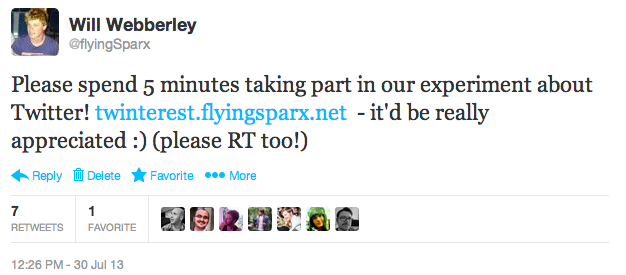
\includegraphics[scale=0.5]{5.Chapter3/Media/organic_advertising.png} 
\caption{Advertising the validation site on Twitter.}
\label{fig:organic_advertising}
\end{figure}

After signing into the read-only application\footnote{Twinterest: source available at https://github.com/flyingsparx/twinterestingness} and beginning the procedure, participants were faced with a series of ten Tweet timelines. The first consisted of the most recent 20 Tweets from the participant's home timeline, and the next nine consisted of user timelines of the participant's friends. Although the selection of friends for the nine user timelines was done at random, a slight bias was applied towards selecting friends with a higher follower count. Due to the nature of scale-free graphs, there are many vertices with few edges, and few with many edges. As such, in order to obtain a more even distribution of user influence, the weighting was necessary to ensure that the scoring mechanism could be validated against a range of users expressing Tweets with a wider variety of retweet counts.

Similar to the initial validations using Mechanical Turk in the previous section, participants were simply asked to select the Tweets that they found to be the most interesting from each of the timelines and were not able to proceed to the next timeline without selecting at least one Tweet. Note that, at this stage, the Tweets being assessed did not have interestingness scores applied to them. A Tweet in a timeline that was selected was considered to be interesting, and those not selected were considered non-interesting.


\subsection{Assigning Scores to the Assessed Tweets}
A total of 580 timelines were assessed through the applciation validations, consisting of 389 contributed to by MTWs and 191 from organic participants. The totals are not precisely divisible by ten since not all participants assessed all of their ten timelines before leaving the application, but no one participant contributed more than ten timeline assessments. In this case, all responses were considered as confident since it was not appropriate under the conditions of the validation test to gain more than one assessment for each Tweet. Although there was likely some friend overlap between the participants, this was not necessarily the case in the vast majority of users assessed. In cases where there the same Tweet was assessed by more than one user the majority vote was chosen, weighted towards positive interestingness decisions in the case of ties. 

\begin{figure}[h]
\centering
\begin{tikzpicture}
 \begin{axis}[
        xlabel=Number of selected Tweets,
        ylabel=Probability,
        grid = major,
        ymax=0.5,
        ymin=0,
        xmin=0,
        xmax=9
       ]
	\addplot[mark=+,only marks,blue]  plot coordinates {
        (1,0.460992908)(2,0.241134752)(3,0.19858156)(4,0.04964539)(5,0.021276596)(6,0.007092199)(7,0.007092199)(8,0.007092199)(9,0.007092199)
    };
\end{axis}
\end{tikzpicture}
\caption{Probability of selecting different numbers of Tweets from each timeline}
\label{fig:num_tweets_selected}

\end{figure}
The validation test resulted in a set of just under 10,000 Tweets, authored by 936 unique users, that had interestingness decisions made on them as part of the assessment of the participants' home timelines and friends' user timelines. These Tweets became the testing dataset $T$, and in order to determine their predicted expected retweet counts using trained classifiers as part of assigning the interestingness scores to each of the Tweets, two procedures were required to take place;
\begin{itemize}
    \item Collect further data on each assessed \textit{author} in order to generate the `user' models, and;
    \item Collect further data on each assessed \textit{Tweet} in order to classify it against the previously-generated global model and the relevant user model.
\end{itemize}
The global model used was the same large model generated during the previous validation tests.

For reasons of privacy, each participant's Twitter API credentials were not maintained by the application and so standard authenticated REST API requests were performed to collect the additional data required. In particular, in August 2013, each of the 936 users representing $\aut{t}{O} \forall t \in T$ were queried under an identical collection scheme to that used as part of the previous validation; information on the author itself and on a sample of the author's followers and friends was retrieved. The collected information was also assigned to each of that user's Tweets $t' \in T$ so that an instance could be built for every $t \in T$ according to the features described in Table \ref{table:globalfeatures}. These Tweets were then classified by the global model and their appropriate user model, which was built from its author's features, in order to eventually produce the two scores. 

It should be noted that if a particular user follows another whose account is protected (see earlier in the thesis for further information on this), then the former user's API credentials can be used to view the latter's information and Tweets. However, since, during the data-collection, a static account was used to query the API, then Tweets and user information for accounts that are protected could not successfully be retrieved. This means that user and Tweet data for these users could not be collected for the purposes of training the user model and testing Tweets against this and the global model, and thus Tweets from protected authors had to be removed from $T$. The numbers stated in this section are those of the \textit{final} dataset after removing these Tweets and users.


\subsection{Results from the Further Validations}
In this section, the patterns observed through the comparison of the Tweers inferred as interesting through the scores and those indicated as interesting by the human participants are analysed. There was no significant difference observed between the accuracy of the scores against the MTWs' and the organic participants' decisions, and thus the combination of both sets was considered in the following analyses. The $\gscore{t}$ was used as the scoring scheme for the analysis in this section.

\subsubsection{Ranking performance in further depth}

\begin{figure}[h]
\begin{subfigure}{.5\textwidth}
    \centering
    \begin{tikzpicture}[scale=0.8]
    \begin{axis}[
            ylabel=Chance of occurrence,
            xlabel=$n$,
            grid=major,
            xmin=0,
            xmax=20,
            ymin=0,
            ymax=1
            ]
       \addplot[mark=+,only marks,blue] plot coordinates{
            (0,0)(1,0.194737)(2,0.310526)(3,0.373684)(4,0.484211)(5,0.557895)(6,0.636842)(7,0.694737)(8,0.747368)(9,0.784211)(10,0.847368)(11,0.878947)(12,0.915789)(13,0.931579)(14,0.947368)(15,0.963158)(16,0.989474)(17,0.989474)(18,1)(19,1)(20,1)
        };    
        \addplot[gray] plot coordinates{
            (0,0)(1,0.05)(2,0.1)(3,0.15)(4,0.2)(5,0.25)(6,0.3)(7,0.35)(8,0.4)(9,0.45)(10,0.5)(11,0.55)(12,0.6)(13,0.65)(14,0.7)(15,0.75)(16,0.8)(17,0.85)(18,0.9)(19,0.95)(20,1) 
        }; 
    \end{axis}
    \end{tikzpicture}
    \caption{In timelines where one Tweet was selected}
    \label{fig:rank-one}
\end{subfigure}
\quad
\begin{subfigure}{.5\textwidth}
    \centering
    \begin{tikzpicture}[scale=0.8]
    \begin{axis}[
            ylabel=Chance of occurrence,
            xlabel=$n$,
            grid=major,
            xmin=0,
            xmax=20,
            ymin=0,
            ymax=1
            ]
       \addplot[mark=+,only marks,blue] plot coordinates{
       (0,0)(1,0.275862)(2,0.405172)(3,0.543103)(4,0.637931)(5,0.715517)(6,0.758621)(7,0.810345)(8,0.836207)(9,0.87069)(10,0.887931)(11,0.913793)(12,0.939655)(13,0.948276)(14,0.948276)(15,0.956897)(16,0.974138)(17,0.982759)(18,0.991379)(19,1)(20,1) 
        };    
        \addplot[gray] plot coordinates{
        (0,0)(1,0.1)(2,0.194736842)(3,0.284210526)(4,0.368421053)(5,0.447368421)(6,0.521052632)(7,0.589473684)(8,0.652631579)(9,0.710526316)(10,0.763157895)(11,0.810526316)(12,0.852631579)(13,0.889473684)(14,0.921052632)(15,0.947368421)(16,0.968421053)(17,0.984210526)(18,0.994736842)(19,1)(20,1)
        }; 
    \end{axis}
    \end{tikzpicture}
    \caption{In timelines where two Tweets were selected}
    \label{fig:rank-two}
\end{subfigure}
\begin{subfigure}{.5\textwidth}
    \centering
    \begin{tikzpicture}[scale=0.8]
    \begin{axis}[
            ylabel=Chance of occurrence,
            xlabel=$n$,
            grid=major,
            xmin=0,
            xmax=20,
            ymin=0,
            ymax=1,
            legend entries={Scoring methodology performance, Random performance},
            legend style={at={(2.4,0.5)}, nodes={right}}
            ]
       \addplot[mark=+,only marks,blue] plot coordinates{
            (0,0)(1,0.282353)(2,0.447059)(3,0.517647)(4,0.682353)(5,0.717647)(6,0.776471)(7,0.823529)(8,0.858824)(9,0.882353)(10,0.905882)(11,0.941176)(12,0.952941)(13,0.976471)(14,0.988235)(15,1)(16,1)(17,1)(18,1)(19,1)(20,1)
        };    
        \addplot[gray] plot coordinates{
            (0,0)(1,0.15)(2,0.284210526)(3,0.403508772)(4,0.50877193)(5,0.600877193)(6,0.680701754)(7,0.749122807)(8,0.807017544)(9,0.855263158)(10,0.894736842)(11,0.926315789)(12,0.950877193)(13,0.969298246)(14,0.98245614)(15,0.99122807)(16,0.996491228)(17,0.999122807)(18,1)(19,1)(20,1)
        }; 
    \end{axis}
    \end{tikzpicture}
    \caption{In timelines where three Tweets were selected}
    \label{fig:rank-three}
\end{subfigure}
\caption{The chance of a participant selecting one of the \textit{highest} $n$ ranked Tweets in the timeline}
\end{figure}

In the previous validation, the performance of the interestingness scores in ranking Tweets was assessed on a per-question basis. The same concept is expanded here to apply a similar assessment of the scores on the present validation test.

In this case, each assessed \textit{timeline} was ranked in order of descending interestingness score in an effort to find the probability of a participant selecting a Tweet occurring in the top $n$ of Tweets. Timelines were up to 20 Tweets long, compared to the five used in the Mechanical Turk questions in the initial validation test, but the scores have again demonstrated that the mechanism is able to effectively rank Tweets. Since the timelines are larger than the questions used before, the chance of a participant selecting multiple Tweets from a timeline was greater, as indicated by Figure \ref{fig:num_tweets_selected}. To illustrate this, the results for this analysis are demonstrated against the appropriate random performance benchmark produced by the different selection criteria.

It is clear that the scores are able to identify interesting information from the noise around it, and so further analyses were conducted into the performance of the scores in detecting \textit{un}-interesting information. In this scenario, each timeline had its Tweets ranked in order of \textit{ascending} interestingness score and calculations were carried out into the probability of participants \textit{not} selecting the \textit{bottom} $n$ interesting Tweets in each timeline.

\begin{figure}[h]
\begin{subfigure}{.5\textwidth}
    \centering
    \begin{tikzpicture}[scale=0.8]
    \begin{axis}[
            ylabel=Chance of occurrence,
            xlabel=$n$,
            grid=major,
            xmin=0,
            xmax=20,
            ymin=0,
            ymax=1
            ]
       \addplot[mark=+,only marks,blue] plot coordinates{
            (0,1)(1,0.908571429)(2,0.828571429)(3,0.742857143)(4,0.662857143)(5,0.582857143)(6,0.564417178)(7,0.5)(8,0.5)(9,0.488188976)(10,0.398305085)(11,0.339449541)(12,0.347368421)(13,0.337349398)(14,0.260273973)(15,0.21875)(16,0.244897959)(17,0.189189189)(18,0.107142857)(19,0.052631579)(20,0)
        };    
        \addplot[gray] plot coordinates{
           (0,1)(1,0.95)(2,0.9)(3,0.85)(4,0.8)(5,0.75)(6,0.7)(7,0.65)(8,0.6)(9,0.55)(10,0.5)(11,0.45)(12,0.4)(13,0.35)(14,0.3)(15,0.25)(16,0.2)(17,0.15)(18,0.1)(19,0.05)(20,0) 
        }; 
    \end{axis}
    \end{tikzpicture}
    \caption{In timelines where one Tweet was selected}
    \label{fig:rank-one2}
\end{subfigure}
\quad
\begin{subfigure}{.5\textwidth}
    \centering
    \begin{tikzpicture}[scale=0.8]
    \begin{axis}[
            ylabel=Chance of occurrence,
            xlabel=$n$,
            grid=major,
            xmin=0,
            xmax=20,
            ymin=0,
            ymax=1
            ]
       \addplot[mark=+,only marks,blue] plot coordinates{
            (0,1)(1,0.854545455)(2,0.745454545)(3,0.645454545)(4,0.545454545)(5,0.427272727)(6,0.38317757)(7,0.336734694)(8,0.276595745)(9,0.224719101)(10,0.159090909)(11,0.111111111)(12,0.130434783)(13,0.064516129)(14,0.055555556)(15,0.020408163)(16,0.024390244)(17,0)(18,0)(19,0)(20,0) 
        };    
        \addplot[gray] plot coordinates{
            (0,1)(1,0.9)(2,0.805263158)(3,0.715789474)(4,0.631578947)(5,0.552631579)(6,0.478947368)(7,0.410526316)(8,0.347368421)(9,0.289473684)(10,0.236842105)(11,0.189473684)(12,0.147368421)(13,0.110526316)(14,0.078947368)(15,0.052631579)(16,0.031578947)(17,0.015789474)(18,0.005263158)(19,0)(20,0)
        }; 
    \end{axis}
    \end{tikzpicture}
    \caption{In timelines where two Tweets were selected}
    \label{fig:rank-two2}
\end{subfigure}
\begin{subfigure}{.5\textwidth}
    \centering
    \begin{tikzpicture}[scale=0.8]
    \begin{axis}[
            ylabel=Chance of occurrence,
            xlabel=$n$,
            grid=major,
            xmin=0,
            xmax=20,
            ymin=0,
            ymax=1,
            legend entries={Scoring methodology performance, Random performance},
            legend style={at={(2.4,0.5)}, nodes={right}}
            ]
       \addplot[mark=+,only marks,blue] plot coordinates{
            (0,1)(1,0.773809524)(2,0.535714286)(3,0.392857143)(4,0.297619048)(5,0.261904762)(6,0.2375)(7,0.151898734)(8,0.12)(9,0.108108108)(10,0.123076923)(11,0.079365079)(12,0.054545455)(13,0.037735849)(14,0)(15,0)(16,0)(17,0)(18,0)(19,0)(20,0)
        };    
        \addplot[gray] plot coordinates{
            (0,1)(1,0.85)(2,0.715789474)(3,0.596491228)(4,0.49122807)(5,0.399122807)(6,0.319298246)(7,0.250877193)(8,0.192982456)(9,0.144736842)(10,0.105263158)(11,0.073684211)(12,0.049122807)(13,0.030701754)(14,0.01754386)(15,0.00877193)(16,0.003508772)(17,0.000877193)(18,0)(19,0)(20,0)
        }; 
    \end{axis}
    \end{tikzpicture}
    \caption{In timelines where three Tweets were selected}
    \label{fig:rank-three2}
\end{subfigure}
\caption{The chance of a participant \textit{not} selecting one of the \textit{lowest} $n$ ranked Tweets in the timeline}
\end{figure}

Although the results showed that, with the different selection criteria, the scores are able to assist in identifying non-interesting information, the difference between this performance and the random selection case is not as significant as with detecting the positively interesting Tweets.


\subsubsection{Crowdsourced timeline selections}

\begin{figure}[h]
\begin{subfigure}{.5\textwidth}
    \centering
    \begin{tikzpicture}[scale=0.8]
     \begin{axis}[
        view={0}{90},
        ylabel=Position of selection,
        colormap/hot,
        grid=none,
        y dir=reverse,
        xticklabels=none,
        xticklabel style=none,
        yticklabel style=none,
        ticks=none,
        separate axis lines,
        y axis line style= { draw opacity=0 },
        x axis line style= { draw opacity=0 },
        draw=none]
      \addplot3[surf] table [row sep=newline] {5.Chapter3/data/heatmap.dat};
      \addplot[black] plot coordinates{       
            (0,6.0743)(19,6.0743)
      };
     \end{axis}
    \end{tikzpicture}
    \caption{Selections made by organic participants}
\end{subfigure}
\quad
\begin{subfigure}{.5\textwidth}
    \centering
    \begin{tikzpicture}[scale=0.8]
     \begin{axis}[
        view={0}{90},
        ylabel=Position of selection,
        colormap/hot,
        grid=none,
        y dir=reverse,
        xticklabels=none,
        xticklabel style=none,
        yticklabel style=none,
        ticks=none,
        separate axis lines,
        y axis line style= { draw opacity=0 },
        x axis line style= { draw opacity=0 },
        draw=none]
      \addplot3[surf] table [row sep=newline] {5.Chapter3/data/heatmap2.dat};
      \addplot[black] plot coordinates{       
            (0,5.825323475)(19,5.825323475)
      };
     \end{axis}
    \end{tikzpicture}
    \caption{Selections made by MTWs}
\end{subfigure}
\caption{Heatmaps illustrating the timeline position of selections made by participants. Mean selection position is indicated}
\end{figure}

A brief study was additionally made into the selections of Tweets made by the participants. Of particular interest is the \textit{difference} in performance between those pariticpants that were paid to take part (the MTWs) and those who took part without being paid (the organic participants), and whether one group was more likely to select Tweets near the top of the timeline without scrolling down to read and select those at the bottom of the timeline. Reasons for this case could be laziness on the behalf of the participant, or simply for speed.

The study revealed that there wasn't a significant difference between the two participant groups. The organic participants, on average, selected the Tweet at position 6.07 in the timeline, and the MTWs selected Tweets at the average position of 5.83 out of 20 maximum available positions.
Whilst these selection position averages are both relatively near to the top of the timeline, it should be noted that the \textit{mean} timeline length was of 14 Tweets, and thus purely average random selections would be made at around the mark of the seventh Tweet.

It is felt, therefore, that there was some bias in both participant groups in that they were both slightly more likely to select Tweets nearer the top of the timeline than scroll down to view, and make interestingness judgments on those, nearer the bottom of the timelines. As with the previous validation tests, it was also possible to demonstrate that the score disparity between Tweets in a particular timeline is greater in cases where only one selection is made by the participants (Figure \ref{fig:disparity2}). 

\begin{figure}
    \centering
    \begin{tikzpicture}[scale=0.8]
    \begin{axis}[
            ylabel=Maximum disparity,
            xlabel=Number of selected Tweets,
            grid=major,
            xmin=1,
            xmax=9,
            ymin=0
            ]
        \addplot[mark=+,only marks,blue] plot coordinates{
            (1,4246.666667)(2,2694.0)(3,2444.0)(4,125.0)(5,29.0)(6,998.6666667)(7,15.0)(8,19.33333333)(9,40.33333333)
        }; 
    \end{axis}
    \end{tikzpicture}
\caption{Relationship between the number of selected Tweets in a timeline and the maximum score disparity of the timeline}
\label{fig:disparity2}
\end{figure}


\section{Chapter Summary}
In this chapter, an improvement over the previous iteration of the Tweet interestingness inference methodology has been introduced, tested, and analysed. Bringing the research into the social structure of Twitter forward from the previous chapter, it was possible to determine areas for improvement and the useful metrics for governing the selection of new features.

\subsection{Interestingness Scores}
The new methodology introduced the notion of scores, which can be assigned to Tweets in order to signify their relative interestingness. These scores are based on the ratio between the popularity of a Tweet, measured by its observed retweet count, and a value representing an \textit{expected} retweet count for the Tweet. The scoring mechanism works such that different types of users, including those ranging across influence and activity frequency\footnote{The activity frequency is how often a user posts Tweets} levels, can have their Tweets assessed on the same scale. 

Two scoring schemes were set up, which are derived from distinct methods for generating the expected retweet count. One method is based on comparing a Tweet's (and its author's) features to a \textit{global} model trained on a large number of Tweets collected from Twitter. The other is generated through the comparison of the Tweet's features to a \textit{user} model trained only on other Tweets posted by that same particular user. Generally, there was found to be a non-significant difference between the performance of the two scores, however, and thus they were both used interchangeably during the validations.

\subsection{Methodology Validations}
Two sets of validations were conducted into verifying the performance and accuracy of the new methodology and the scores it produced - one in which Tweets were placed into questions on Amazon's Mechanical Turk, in which MTWs were asked to select the most interesting Tweets; and another, in which participants were asked to sign-in through Twitter and then assess Tweets from users they actually follow.

In the first case, the participants shared no connection with the authors of the Tweets they were assessing (except in the case of coincidences), and were therefore assessing Tweets on a \textit{global} interest level. In particular, this largely involves determining the interesting information from the noise around it. In the second set, information \textit{relevance} came more into play, since participants were assessing Tweets from users they have already declared an interest in (through the action of following).

In both test cases, the validations showed the scores to be able to appropriately label Tweets according to interestingness in a variety of different ways. The second test included an analysis demonstrating that the scores are more efficient at determining interesting Tweets than \textit{un}-interesting Tweets, the latter of which would be useful in deciding on a set of Tweets to discard from an interesting set. 

\subsection{Improvements and Qualities}
The newly introduced methodology presents several improvements over that described in the previous chapter. In particular, the performance of the scores have shown a large accuracy improvement in determining interesting information. The previous method also did not take into account \textit{how} interesting a particular Tweet may be, and was only able to make a binary interesting/uninteresting decision for each Tweet.

Another large improvement is the ability of the scoring method to be applied to a much wider range of Tweets. The previous method was realistically unable to assess Tweets from users with more than 300 or so followers due to data collection inefficiency, the time taken, and the computational complexity involved in simulating large user graphs. The new method can be used to assign scores to Tweets in a more ``on demand'' fashion, where only a small amount of information for each Tweet is required in order to generate the features needed to predict the estimated retweet counts. The scores also allow Tweets from many different sources to be assessed on the same scoring scale, meaning that Tweets on a mixed timeline can be appropriately compared to one-another, as demonstrated by the second set of validations.

\chapter{Assessment and Conclusions}
Here is provided an overview and assessment of the work conducted in this thesis, bringing together the ideas from the initial research and how these have helped in developing the methodologies introduced in later chapters. The validations from the methods are further assessed, followed by an explanation of how the research forming them may be taken further in potential future projects. Finally, an overview of the thesis in terms of its contributions is described.


\section{Analysis of Research and Results}
In this thesis, the research behind the development of an effective interestingness predictor has been described. The relative successes of the methodology and its advantages over its previous iterations have been illustrated through in-depth analyses of its performance in various situations.

Following is an analysis of the research carried out over the main stages described in the primary chapters of this thesis.

\subsection{Retweeting \& the Twitter Structure}
Initial research was conducted into the act of retweeting and Twitter in general for the purposes of providing a background and foundation for the later work. In particular, the properties of retweet groups and the behaviour of the users within them was demonstrated. During the review of the relevant literature in the field, it was suggested that a Tweet's popularity cannot generally be directly tied to the Tweet's interestingness due to factors relating to user \textit{influence}.

Agreeing with other research in the area, it was demonstrated that retweet groups can have widely ranging sizes and depth. This observation takes into account that retweets can, themselves, be retweeted, and that retweet groups do \textit{not} consider the followships between the set of users they represent. Retweet groups were found to present an average \textit{maximum} path-length of around two, and the longest maximum path found in the dataset collected from retweets on the public timeline was of length nine. This demonstrates a significant penetration through the social graph, especially considering the `real' world's six degrees of separation, and that social networks often exhibit a social graph even more closely connected than this.

It was found that the chance of a retweet occurring was much greater in cases where the retweeter follows the author of the original Tweet. As retweet pathways become longer, the chances of the final retweeter following the original author diminishes over the distance, demonstrating strong correlations between the edges separating users on the retweet graph and those on the social graph. These experiments were conducted using a trained logistic regression to predict a retweet outcome decision for each user who received a particular Tweet during simulations of Tweets through each structure type.

The correlations and results from the explorative analyses on the social structure and the arrangement of users on the social graph indicated that the social structure of Twitter clearly affects the propagation of retweets and that this property could provide a useful way of estimating Tweet interestingness. This triggered research focussed on examining the differences in propagation patterns in order to demonstrate that each structure type can present very different retweet propagation patterns. Because the propagation pattern difference at this structural level was so large, it was decided that this could be a basis for an interestingness inference methodology. This method utilised the same research and algorithms behind those used in the graph structure analysis to predict a retweet count for a given Tweet within a graph of connected users, and worked through a simple comparison between this predicted value and the \textit{observed} retweet count of the Tweet. This method was not shown to perform particularly well in the validation tests conducted, and thus improvements were necessary before any further analyses were made.


\subsection{Interestingness Scores}
Improvements over the previous methodology were based around the introduction of interestingness \textit{scores}, with which Tweets could be ranked according to the ratio of their observed and expected popularities, and where if the observed popularity is proportionately larger than the expected popularity, the score for that Tweet would also be proportionately greater. This in itself provides many benefits over the previous system, which was unable to provide any indication over \textit{how} interesting a Tweet is.

The prediction of the estimated retweet count was altered so that they could be generated directly through the use of a Bayesian network machine learning classifier, which made predictions based on a larger set of Tweet and environmental network features. These features could be collected much more efficiently from Twitter's REST API, illustrating another advantage in terms of the ease with which predictions (and thus score assignations) can be made. 

Furthermore, the efficiency stretches to providing a more universal approach, allowing Tweets from most users on Twitter to be evaluated equally and on the same scale, since the complexity of any part of the assignation process is not affected by the influence or other properties of the author user. 

A Bayesian Network was chosen for the methodology improvements due to its relative advantages over the other assessed classifiers, as highlighted by Table \ref{table:classifierperformance}. Although the logistic regression performed almost as well as the Bayesian Network in the cross-validations, its training time, especially with the full dataset, meant that it would be unsuitable, especially if user models are to be generated on-demand. Logistic regression was more appropriate in the earlier work described in Chapter 4, in which of concern was its ability to produce a retweet \textit{probability} from a set of binary feature values. 


\subsection{Validation}
Producing the scores partially relies on the initial accuracy of making retweet predictions in the \textit{general case}, using cross-validation tests on the Bayesian network classifier and the binning policy of retweet counts explained in the previous chapter. The performance of each factor, and the accuracies achieved, are highlighted in Tables \ref{table:classifierperformance} and \ref{table:binperformance} respectively.
%, which demonstrated that a decent precision and recall could be obtained in cases using up to between 15 and 20 nominal bins. Although the binning algorithm was responsive in terms of the range and distribution of retweet counts in the set being analysed, it was aimed to achieve a projected bin count of 10 in the case of producing the global model. When generating the user-specific classifier models, the number of bins ranged largely depending on the relative influence of each user, as described in more depth earlier.

The mention of the ``general case'' is important, since the methodology is designed to discover Tweets which do \textit{not} fit this case, as these would be the Tweets which have a greater (or smaller) retweet count than expected, and would therefore be the Tweets which would contribute negatively to the aforementioned performance analyses of the prediction method. As such, if all Tweets fit their general cases as given by their features and the features of their authors, then the general performance of the cross-validations on the classifier could be greater, but then no interestingness inferences could be made.

Two main human validation tests were conducted into the performance of the scoring mechanisms provided by the improved methods; one based on interestingness decisions from non-related participants, and another based on decisions from Twitter users to whom the Tweets assessed are more directly relevant, as denoted by the followships of the author users. These validations expressed a good performance of the scoring scheme in a variety of ways, from the ranking of Tweets in order of interestingness through to analyses into the motivation of Tweet selection from the \textit{disparity} of Tweet scores in the timeline.

\subsection{Results Overview}
Here (Table \ref{table:final_overview}) is provided an overview of the results from the final validations conducted in this thesis.

\begin{table}{H}\footnotesize
\begin{center}
    \begin{tabular}{l | l}
        Result & Description\\
        \hline
        \hline
        \hline   
    \end{tabular}
\caption{Overview of final validation results.}
\label{table:final_overview}
\end{table}



\subsection{Methodology Evaluation}
The Background chapter of this thesis described other similar research in this area along with the strengths and weaknesses of each. Whilst this included research into retweet decision and count predictions, they are often quite similar to one another, and these goals are not the primary focus of the work in this thesis. Instead, research into information interestingness with regards to Twitter will now be evaluated against the methods outlined in this thesis.

\citet{gransee12} introduced a system for scoring Tweets based on a na{\"i}ve Bayesian classifier. The authors' learner was concerned only with textual cues for producing a score, and thus the method is based on semantics. The learner was trained using a set of Tweets from a particular author, with each Tweet being assigned a score based, similar to the work in this thesis, on the distance between the observed retweet count of the Tweet and the single \textit{baseline} retweet count for the Tweet's author at that particular time. Words in unseen Tweets are then scored individually according to the scores of Tweets the words have previously been seen in, which, when averaged, generates a score for the unseen Tweet.

The scoring method discussed in this thesis is superior to the methodology described by \citet{gransee12} in a number of ways. Firstly, the method requires a pre-built dictionary of words to be generated and scored for each user before a model can be trained and any scores can be assigned, meaning that it is not possible to carry out on-demand assignations of scores to Tweets. Additionally, a baseline retweet count needs to be maintained for each user assessed for specific time-intervals, causing the necessity of periodically updating the word dictionary in order to reflect the change in baseline. The authors admit that their methods work better when Twitter users are more predictable and use similar words across Tweets. The global model discussed in this thesis is able to represent snapshots of projected Tweet popularity for many types of users, and is therefore re-usable for a single user as he/she gains or loses influence, and does not require regeneration. Finally, assessments were only made for the \textit{top} 175 users on Twitter, with no indication of its performance on users who are less influential and typically receive far fewer retweets per Tweet and users who do not Tweet enough in each time-frame for a suitable baseline value to be calculated. Influential users are generally subject to smaller fluctuations in the social graph, as additional followers wouldn't have such a large impact, and thus the retweet count baseline wouldn't vary as often as with less influential users. Therefore it would be more difficult to apply this method to Tweets from `normal' (or less influential) users.


The semantic scoring of Tweets was also considered by \citet{alonso10}, but with a focus on determining non-interesting information. In this case, the authors used a scoring scheme that assigned an integer value to each Tweet of between 0 and 5. However, their results are largely based on simply marking a Tweet as interesting if it contains a URL, which, again, does not allow the method to be appropriately applied to a wider range of Tweets. Crowdsourcing is used as part of obtaining human input for determining interestingness, but the MTWs are instructed on what to class as interesting instead of allowing participants more reign on what constitutes the \textit{most} interesting. Generally, these features are not comparable to those in the methods discussed in this thesis, since the authors are more concerned with finding \textit{un}interesting Tweets to be disregarded from a stream, have a limited scoring range and do not conduct as rigorous validations into their results. Despite achieving some accurate results, the methods cannot be used on such a wide variety of Tweets as is available on Twitter.

Finally, \citet{lauw10} presented a study that used a clustering algorithm to estimate a Tweet's \textit{quality} based on a function of a Tweet's audience size and its relation to other similar Tweets. The authors' research is based around news stories, in that Tweets `belonging' to the same event are clustered together and are assigned a quality depending on the size and `importance' of the cluster. Despite the similarities in terms of assigning a quality to clusters and Tweets, the authors do not take into consideration many of the factors discussed in this thesis (including the notion of timeline `slip' discussed in Chapter 4, which is relevant to their work) and the verifications conducted into the performance of their methods are not rigorous enough to prove that the quality level assigned to each cluster or Tweet is accurate or appropriate.


\section{Further and Future Work}
There are various ways in which the work and research in this thesis could be taken further in extended work and projects.


%\subsection{Marketing}
% Maybe remove this section
%As part of the procedure for assigning scores to a Tweet, it was necessary to produce an \textit{expected} retweet count for it. This is a prediction based on the Tweet's user and author features and the similarities of these to previously-seen Tweets. Although the interestingness inferences are based on the expected count being different from the actual retweet count, it was shown that the classifier and binning algorithms used demonstrated a good performance in classifying the retweet outcome for a given Tweet. 

%As such, it is sensible to assume that this predictor could be taken further in assisting Twitter users in constructing Tweets which are likely to attract more retweets. Before posting a Tweet, a system could use a trained classifier to indicate how many retweets the Tweet is likely to receive. With respect to the interestingness scores produced by the full methodology, these could be useful for retrospectively returning feedback to users in order to highlight the Tweets that were more popular than expected and to perhaps illustrate any common features found in Tweets that were more popular than those that weren't. 

%Of course, isolating the notion of popularity from the static features of a Tweet in the general case forms part of the motivation for this research, but the value of features for some users may have more of an effect on their retweet receipts than on other users. For example, a Twitter account representing a news service is more likely to receive retweets of Tweets that contain a URL than an account representing a parody celebrity account, who is likely to obtain retweets more through the wording and relevance of the content of the actual Tweet.


\subsection{Building on the Social Structure}
Chapter 4 of this thesis included research into the social structure of Twitter and the role this played in the retweet propagation patterns of the information flow within it. The impact of the structural changes on the propagation pattern led the way in building the initial interestingness inference methodology, which was based on simulating Tweets and retweet decisions through social structures reflected directly from Twitter.

The method had many drawbacks, as described earlier, but mainly these were due to its inefficiency in terms of the amount of data necessary in order to construct the local networks, which included all the users and edges within two hops of the source author user. Nodes three hops or more from the source were prohibitively complex to collect and implement due to the scaling nature of the Twitter social graph, and two was considered sufficient as it was the average \textit{maximum} path-length of Tweets analysed in Chapter 3. Despite this, the limitations in data collection meant that Tweets could only realistically be simulated for users with much smaller local networks, and thus the methods could not be applied to a wide variety of Tweets on Twitter or have inferences made on demand.

The research in this thesis then followed a different path in an attempt to solve the presented problems, but there are ways in which the previous method could be improved more directly. One way, in particular, would be to attempt to \textit{infer} or `estimate' a user's local network from a set of its immediately-available parameters. Analytical results from this first methodology highlighted correlations between a user's follower count and the size of the user's local follower network, and a correlation between the size of this local network and the edge density of the users within it, as illustrated by Figures \ref{fig:network-followers} and \ref{fig:network-density}.

\begin{figure}[h]
\begin{subfigure}{.5\textwidth}
    \centering
    \begin{tikzpicture}[scale=0.8]
    \begin{loglogaxis}[
            ylabel=$\foc{\aut{t}{O}}$,
            xlabel=$|N|$,
            grid=major,
            xmin=1E4,
            xmax=1E6
                       ]
       \addplot[mark=+,only marks,blue] plot coordinates{
            (15244,28)(20273,38)(26943,56)(28279,41)(39192,56)(58650,80)(67585,125)(90366,170)(109982,230)(112070,135)(118854,279)(132497,273)(184158,291)(258252,388)(352661,617)(368389,628)(561100,928)(666690,900)        
        };    
    \end{loglogaxis}
    \end{tikzpicture}
    \caption{Relationship between local network size ($|N|$) and the follower count of an author of Tweet $t$.}
    \label{fig:network-followers}
\end{subfigure}
\quad
\begin{subfigure}{.5\textwidth}
    \centering
    \begin{tikzpicture}[scale=0.8]
    \begin{loglogaxis}[
            ylabel=$d$,
            xlabel=$|N|$,
            grid=major,
            xmin=1E4,
            xmax=1E6
            ]
       \addplot[mark=+,only marks,blue] plot coordinates{
            (352661,4.49E-06)(37084,3.20E-05)(10631,0.000103613)(184158,6.97E-06)(39192,2.74E-05)(90366,1.62E-05)(33520,4.00E-05)(72123,1.71E-05)(112070,9.40E-06)(72069,1.70E-05)(132497,9.19E-06)(368389,4.06E-06)(358200,5.29E-06)(118854,1.10E-05)(109982,1.10E-05)(15244,7.50E-05)(382357,3.39E-06)(15273,7.03E-05)(106877,1.03E-05)(28279,3.72E-05)(18366,5.84E-05)(666690,2.40E-06)(205417,5.21E-06)(26943,3.87E-05)(19385,6.16E-05)(561100,2.61E-06)(58650,1.75E-05)(258252,5.11E-06)(106247,1.04E-05)(32300,3.22E-05)(67585,1.63E-05)
        };    
    \end{loglogaxis}
    \end{tikzpicture}
    \caption{Relationship between local network size ($|N|$) and local graph edge density ($d$).}
    \label{fig:network-density}
\end{subfigure}
\caption{Plots illustrating indirect correlations between an author user's follower count and the edge density of the author's local network}
\end{figure}

A graph's edge density can be calculated as a function of the number of nodes and edges existing within the graph;
\[
    d = \frac{|E|}{|N|(|N| - 1)}
\]

This suggests that a user's follower count could be used to indirectly estimate the edge density of that user's local follower graph. Since Figure \ref{fig:real-scalefree} showed the similarities, along with other research covered in the Background chapter, between the structure of Twitter's social graph and that of a similarly-sized scale-free network, it is indicative that a faux scale-free network could be generated with a provided edge density and size in such a way as to reflect the user's own local network. Although this would not be an intricate mapping of the users and edges existent in reality, it would provide an appropriate size and density of edges between the nodes, within which Tweets could be propagated and examined.

Through generating a graph structure in this fashion, then there is no need to collect the local network information for each user to be assessed, since a faux graph could simply be created on the fly, and Tweets from more influential users could also be simulated (depending on the computational complexity of the generation algorithm and simulator). The \textit{accuracy} of the interestingness inference could then be improved through a larger training set, the use of more features for handling the decisions, or by introducing further routines to make the simulations and the decisions more realistic. 


\subsection{Taking the Scoring Methodology Further}
There are various ways in which research could be carried out into the methodologies behind the scoring mechanism used in the interestingness inferrer discussed in Chapter 5. In particular, one could be to research into `unnecessary' edges between users in OSNs. The final validations conducted on this method involved participants assessing the Tweets they'd naturally receive onto their home timeline as they are from users that they already \textit{follow}. 

However, as has been made clear at points in this thesis, not \textit{all} the information a friend posts is likely to be interesting, and that particularly interesting information from a particular source is likely to be retweeted more than less interesting information posted by the same source. 
%If a particular destination user finds only a small subset of Tweets from a source to be interesting, and that these Tweets are therefore more likely to be retweeted by other users also following the source, then is there a non-direct pathway available between the source and the destination user that the interesting Tweets could be passed down?

\begin{figure}[h]
\centering
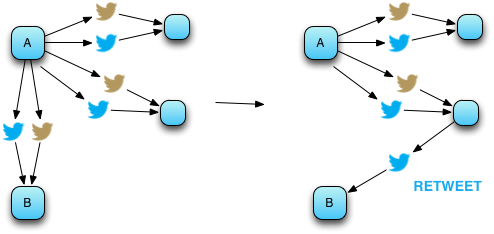
\includegraphics[scale=0.8]{6.Conclusions/Media/retweet_path.png} 
\caption{Using `filtered' edges to improve interestingness precision.}
\label{fig:removed_link}
\end{figure}

Therefore, the interestingness scores could be used to allow users to form conditional followships to other users, down which only interesting Tweets are sent. Figure \ref{fig:removed_link} initially shows user B receiving all of the Tweets from user A down a normal Twitter followship edge. However, if user B instead followed user A through a `filtered' edge, then only Tweets with a sufficient interestingness score would be received. Under this type of scheme, user B avoids receiving the uninteresting Tweets from A, thus increasing the chance of noticing the interesting ones.

%If this is the case, as with Figure \ref{fig:removed_link}, then the link representing the followship between the destination user (B) and the source user (A) could be unnecessary, since user B is receiving noise from user A, but the interesting information produced by user A could still reach B through retweets carried out by other followers of A. 

Of course, this system does require a set of users to be already following A in order to initially generate scores for each Tweet, but it does illustrate an interesting path for future research. Whilst largely hypothetical at this stage, it would provide an interesting extension to the research carried out in this thesis, in that interestingness scores could be used to assign thresholds of interestingness to users with the aim of discovering whether interesting Tweets could still be propagated to the extent that they deserve, yet by simultaneously reducing the propagation of noisy information. 

Since it has been explained how a user's followships act as a `search term' for information retrieval on Twitter, by finding ways of forwarding interesting information to users who do not directly (or `traditionally') follow a source, then it is clear how this could pave a way for enabling interesting and \textit{relevant} information can be delivered to users, yet without them having to look for it or know about its existence in the first place.


\section{Conclusions}
The work in this thesis was carried out with the aim of researching a methodology that is able to suitably infer interesting information in Twitter. Although the research has focused on Twitter as a platform for information dissemination, the motivation for this research stems from the \textit{noise} observed every day in all online social networks that support information propagation, including those such as Facebook and Tumblr.

The research processes culminated in the development of a method that ranks Tweets by assigning a score indicating an estimated level of interestingness based on a function of its perceived popularity. The methods were verified through the use of crowd-sourced validation tests covering the notions of general interestingness (in terms of identifying it from `noisy' information) and of more \textit{relevant} interestingness (through assessments of Tweets authored by more relevant users).

Analyses into the validation tests demonstrated the process by which users are able to identify interesting information and showed that the scoring mechanism is able to effectively rank Tweets in an appropriate order of interestingness in both mixed timelines and in timelines of Tweets authored by the same user. The scores can be applied to Tweets from all users on the same scale, meaning that inferences are not limited to a specific subset or type of Tweet.

The methods are open enough and use resources that are mostly common to many similar social networks. For example, ``shares'' and ``reblogs'' can be examined as the propagation mechanisms in Facebook and Tumblr, respectively, in attempts to apply the same scoring schemes to other platforms.


\section{Contributions}
Throughout the earlier chapters of this thesis, work has been conducted towards answering the hypothetical questions asked in Section \ref{section:research_questions} in the Introduction. The research has highlighted the inappropriateness of using retweet counts alone in indicating interestingness, and has shown the impact of the layout of users on the social graph on message propagation and how this can be useful for estimating Tweet interestingness. In particular, the questions are now answered more formally.

\textit{\textbf{RQ1} - Does Tweet popularity, measured in terms of retweets, \textbf{define} interesting (or non-`noisy') information?}\\
The number of retweets a particular Tweet receives cannot appropriately be used for defining interesting information. A Tweet that has been retweeted at least once is not necessarily interesting.

\textit{\textbf{RQ2} - Can Tweet popularity, measured in terms of retweets, \textbf{be an indicator} of interesting information?}\\
The number of retweets a Tweet has achieved is not alone indicative of its level of interestingness. The overall retweet count of a Tweet is produced as a function of its author's influence, and therefore Tweets written by different authors cannot have their Tweets' interestingness measured on the same scale.

\textit{\textbf{RQ3} - Is the arrangement of Twitter's social graph an important factor in retweet propagation, and thus perceived popularity?}\\
The layout of users and the edges connecting them on the social graph has been shown to strongly affect the permitted propagation of Tweets; some structures facilitate retweet spread, whilst others throttle it. The edge density also partially dictates users' influence levels, in that those users who are assigned a larger in-degree are more likely to achieve more retweets due to the magnitude of spread of the original Tweets. This importance was brought forward to the later work in identifying interesting Tweets.

\textit{\textbf{RQ4} - Can Tweet interestingness be inferred \textbf{non-semantically}?}\\
Chapter 5 showed that a Tweet's interestingness can be determined through a study of the Tweet's features and those of its author and the latter's relationship to others on the social graph. The inferences are therefore non-semantic, since they do not make any attempt to understand the content of individual words or phrases in the Tweets' contents. The method was also demonstrated to be suitable for ranking Tweets in order of interestingness \textit{level}, so that Tweets estimated to be more interesting could be shown at a higher priority.

As part of the research, several contributions to social media analytical research have been made, which have been discussed in the relevant chapters of the thesis and are summarised below. 

A comprehensive survey is carried out into relevant literature in information propagation in online social networks, along with evaluations and assessments of some of the research more specific to inferring interestingness.

Retweet properties and the way they are influenced by the social graph are thoroughly researched in order to provide a general background and understanding of the notions relating to propagation in online social networks, propagation and information penetration, Tweet `audience', and how these factors are related to the arrangement of users on the social graph. The definition of terms, such as `retweet group' and `maximum path-length' are useful for discussing various properties relating to retweeting on Twitter.

An investigative study is made into the use of machine learning techniques and classifiers in the field of social media, and the ways in which they can be useful for different purposes.

Finally, a numerical `definition' (or quantification) of estimated interestingness is contributed. A method for suitably predicting estimated retweet counts as dynamically nominal categories is described, implemented and verified, leading to the development of a method for assigning interestingness scores to Tweets as part of an effort to support the ranking of Tweets and of highlighting interesting Tweets from the noise of everyday communication on Twitter.


%\chapter*{Appendices}
%Source code, further diagrams, ideas, etc.

%%%%% BACK STUFF 
\backmatter

\def\baselinestretch{1.24}\normalfont

\bibliographystyle{plain}
\bibliography{includes/library}

\end{document}
